\documentclass[11pt]{book}
\usepackage[T1]{fontenc}
\usepackage[utf8]{inputenc}
\usepackage{amsmath}
\usepackage{array}
\usepackage{geometry}
\usepackage[hidelinks]{hyperref}
\usepackage{amssymb}
\usepackage{tikz}
\usetikzlibrary{arrows.meta,positioning,calc}
\geometry{letterpaper, margin=1in}
\raggedbottom

\title{High-Performance Computer Architecture\\A Concise Review Textbook for Chapters 1--10, Cache Simulation, and Advanced Topics}
\author{ECE 4100/6100}
\date{Spring 2026}

\begin{document}

    \maketitle
    \tableofcontents

    \chapter*{Scope and Topic Map}\label{ch:auto-001}
\addcontentsline{toc}{chapter}{Scope and Topic Map}


\section*{How to Use This Text}\label{sec:auto-001}
Chapters 1 through 10 provide topic depth with definitions, equations, and worked examples.
Chapter 5 provides integrated synthesis and cache-simulation context.
Chapter 6 develops dynamic instruction-level parallelism mechanisms such as superscalar scheduling and out-of-order execution.
Chapter 7 develops compiler-scheduled instruction-level parallelism through very long instruction word (VLIW) execution and software pipelining.
Chapter 8 develops multiprocessor organization, coherence, and parallel programming models.
Chapter 9 develops atomic synchronization, transactional-memory ideas, and memory-consistency semantics.
Chapter 10 develops parallel interconnection-network topologies, routing, flow control, and switch fabrics.
Appendix~\ref{ch:advanced-topics} summarizes the advanced-topics lecture on quantum-computing architecture and superconducting processor research.
Appendix~\ref{ch:final-review-checklist} provides a compact final-review checklist and clarification guide.


\section*{Cross-Chapter Reading Paths}\label{sec:cross-chapter-reading-paths}
\begin{enumerate}
    \item Readers who want the performance-and-memory foundation should begin with Chapters 1 through 3 and then read the first part of Chapter 4.
    \item Readers focused on control hazards, prediction, and data hazards should concentrate on the middle and later sections of Chapter 4.
    \item Readers focused on instruction-level parallelism should read Chapter 6 for dynamic ILP and Chapter 7 for compiler-scheduled ILP\@.
    \item Readers focused on simulator-style interpretation and consolidated worked checks should use Chapter 5 alongside the detailed discussions in Chapters 3, 4, and 6.
    \item Readers focused on thread-level parallelism, coherence, and shared-memory multiprocessors should continue from Chapters 1 and 2 into Chapters 8 through 10.
    \item Readers reviewing the advanced-topics final-exam material should read Appendix~\ref{ch:advanced-topics}.
    \item Readers doing a last comprehensive review should use Appendix~\ref{ch:final-review-checklist} to identify weak concepts, then return to the relevant chapter sections.
\end{enumerate}


\section*{Topic Coverage Map}\label{sec:auto-002}

\paragraph{Chapter 1: Introduction}\label{par:auto-001}
Coverage includes speculation with and without prediction, grain sizes of parallelism (bit, instruction, thread, and inter-program), Flynn taxonomy, single instruction, multiple data (SIMD) versus multiple instruction, multiple data (MIMD), pipelining as temporal parallelism, and the distinction between packed-word SIMD and pipelined vector operations.

\paragraph{Chapter 2: Performance Evaluation}\label{par:auto-002}
Coverage includes throughput versus runtime, the central processing unit (CPU)-time equation in terms of instruction count (IC), cycles per instruction (CPI), and cycle time, reduced instruction set computer (RISC) versus complex instruction set computer (CISC) tradeoffs, Amdahl's and Gustafson's laws, and correct use of arithmetic versus harmonic means.

\paragraph{Chapter 3: Cache Memories}\label{par:auto-003}
Coverage includes static random-access memory (SRAM) versus dynamic random-access memory (DRAM) and bit-line delay, locality, hierarchy levels, virtual-memory terminology and its analogy to caching, average access time (AAT), the three C's of misses, cache geometry and construction, replacement and write policies, insertion-policy choices such as MIP and LIP, prefetching strategies including Markov and hybrid schemes, techniques to improve miss rate, miss penalty, and hit time, simulator-style hierarchy statistics, and compiler/data-layout effects.

\paragraph{Chapter 4: Pipelining}\label{par:auto-004}
Coverage includes instruction fetch / instruction decode / execute / memory / write back (IF/ID/EX/MEM/WB) behavior, speedup equations, cycles per instruction (CPI) stall modeling, the principle that program behavior plus hazards produces stalls, structural and control hazards, delay and squash-slot ideas, branch target buffer (BTB) behavior with and without tags, return-address stack (RAS) behavior, direction-prediction heuristics, and dynamic predictors including one-bit and Smith-counter schemes, GShare, GSelect, Yeh/Patt, perceptrons, hybrid tournament selection, and delayed predictor-update timing.

\paragraph{Chapter 5: Integrated Synthesis and Cache Simulation Concepts}\label{par:auto-005}
Coverage includes integrated synthesis, worked pipeline calculations, hierarchy semantics, prefetching, and interpretation of simulator-style cache, branch, and average access time (AAT) statistics.

\paragraph{Chapter 6: Dynamic ILP, Superscalar Scheduling, and Out-of-Order Execution}\label{par:scope-ch6}
Coverage includes cycles per instruction (CPI) versus instructions per cycle (IPC) interpretation, instruction-level parallelism (ILP), historical superscalar context, fire/complete ordering models, scoreboarding and busy-bit scheduling, function-unit latency considerations, Tomasulo-style reservation stations, physical register files, result buses, register renaming intuition, precise versus imprecise exceptions, reorder buffer (ROB) and future-file organization, checkpoint/repair recovery, simulator-style fetched/retired and queue-pressure counter interpretation, and the security consequences of speculative out-of-order execution.

\paragraph{Chapter 7: Compiler-Scheduled ILP and Software Pipelining}\label{par:scope-ch7}
Coverage includes compiler-scheduled very long instruction word (VLIW) execution, dependence-graph and list-scheduling ideas, zero-no-op multi-op encoding with tail and pause fields, software pipelining and iterative modulo scheduling, and memory disambiguation.

\paragraph{Chapter 8: Multiprocessors, Interconnects, and Cache Coherence}\label{par:scope-ch8}
Coverage includes shared-memory versus message-passing organization, standalone multiprocessors versus accelerator systems, buses versus point-to-point links, the cache-coherence problem and its formal properties, shared-cache versus directory-based versus snooping solutions, MSI coherence states and transactions, MESI/MOESI/MOESIF refinements including \texttt{E}, \texttt{O}, and \texttt{F}, transient coherence states, directory-entry structure and message flow, limited and distributed directory organizations, sharing patterns and false sharing, and shared-memory programming support through locks, barriers, and atomic synchronization primitives.

\paragraph{Chapter 9: Atomic Synchronization, Transactional Memory, and Memory Consistency}\label{par:scope-ch9}
Coverage includes the distinction between coherence states and full protocol behavior, abort-versus-intervene transfer policies, load-link / store-conditional, fetch-and-op and fetch-and-add primitives, dynamic work claiming, tree and tournament locks, sense-reversing barriers, hardware barrier intuition, transactional-memory execution and aborts, and the distinction between coherence and memory consistency, including strict consistency, sequential consistency, relaxed consistency, data races, and synchronization ordering through fences and acquire/release style semantics.

\paragraph{Chapter 10: Parallel Interconnection Networks}\label{par:scope-ch10}
Coverage includes the distinction between direct and indirect topologies, hypercube organization and Gray-code intuition, $k$-ary $n$-dimensional meshes and tori, physical-layout constraints and wire-length balance, bisection bandwidth, crossbars and dance-hall style switching, multi-stage interconnects such as omega networks, perfect-shuffle wiring, deterministic versus adaptive versus oblivious routing, packets versus flits, and the progression from store-and-forward to cut-through, wormhole, and virtual-channel flow control.

\paragraph{Appendix D: Advanced Topics}\label{par:scope-appd}
Coverage includes quantum computers as accelerators, decoherence, imperfect control, NISQ limits, fault-tolerant logical qubits, reversible phase-oracle intuition, superconducting-circuit constraints, compiler-scheduled dataflow execution, operand queues, barrel processing, and combined single-thread/throughput-oriented superconducting processor organization.

\paragraph{Appendix E: Final Review Checklist}\label{par:scope-appe}
Coverage includes a comprehensive concept checklist, review clarifications for tiling, iterative modulo scheduling, memory consistency, barriers versus locks, and bisectional bandwidth, plus fast self-check prompts.

    \chapter{Introduction}\label{ch:auto-002}

\section{What Computer Architecture Is}\label{sec:auto-003}
Computer architecture is the discipline of designing computing systems that execute real workloads efficiently under practical constraints.
In this course context, architecture means deciding how a processor and memory system should be organized so that useful work is completed quickly, reliably, and within power and cost limits.
It is important to separate this from neighboring fields.
Architecture is not transistor fabrication, circuit layout, or process chemistry, even though those influence what architects can build.

Every architectural decision is a tradeoff among competing goals.
A design that minimizes latency for one task may reduce throughput for a server-style workload.
A design that aggressively improves performance may consume more energy or require expensive cooling.
A design that is elegant on paper may be too costly in area or too difficult to verify at scale.
For this reason, architecture is best treated as constrained optimization: choose structures and policies that best match the target application while respecting implementation limits.

\section{Core Methods: Parallelism, Speculation, and Prediction}\label{sec:auto-004}
Most performance techniques in modern processors can be traced to three closely linked ideas: \textit{parallelism}, \textit{speculation}, and \textit{prediction}.
\textit{Parallelism} increases performance by doing multiple useful operations at the same time.
\textit{Speculation} increases performance by doing work early, before the machine is fully certain that this work will be needed.
\textit{Prediction} estimates uncertain future behavior (for example branch direction or branch target) so speculative work is directed toward the most likely path.
Prediction is not a third independent speedup method; it is a tool that makes speculation more selective and efficient.

\subsection{Speculation Without Prediction}\label{subsec:auto-001}
Speculation does not require a learned predictor.
A processor can speculate by optimistic overlap: continue execution under the assumption that an operation will complete normally, and recover only if that assumption fails.
This is useful because waiting for every operation to retire before moving on would underutilize the pipeline.

\paragraph{Example: write buffer}\label{par:auto-006}
A write buffer is a standard example.
When the core executes a store, it can enqueue the write and continue with subsequent instructions before that store reaches the lower memory hierarchy.
If the store later encounters a fault condition, architectural recovery and exception handling restore correctness.
The processor did not predict branch direction or data values in this case; it simply advanced optimistically to avoid stalling.

\subsection{Speculation With Prediction}\label{subsec:auto-002}
When prediction is added, speculation becomes more selective and usually more efficient.
The processor estimates likely future behavior, executes along the estimated path, and commits the work only if the estimate is correct.

\paragraph{Example: branch prediction}\label{par:auto-007}
Branch prediction is the canonical case.
If the predictor guesses that a branch is taken, instruction fetch and decode proceed down the predicted target path immediately.
A correct guess keeps the front end busy and reduces control-hazard stalls.
An incorrect guess forces the machine to squash the speculative instructions and restart on the correct path, which introduces a misprediction penalty.
The basic tradeoff is straightforward: high prediction accuracy yields high performance; low accuracy can erase the benefit of speculation.

\section{Parallelism by Grain Size}\label{sec:auto-005}
Parallelism is best understood by \textit{grain size}, meaning the amount of work grouped into one concurrent unit.
At the smallest scale, bit-level parallelism appears in wide datapaths and arithmetic logic that operate on many bit positions at once.
A 64-bit adder, for example, processes far more state per cycle than an 8-bit design because the hardware width itself exposes more fine-grained parallel work.

At \textit{instruction-level parallelism (ILP)}, the machine overlaps independent instructions within a thread.
Superscalar issue, out-of-order scheduling, and pipelining all exploit ILP\@.
Consider two arithmetic instructions: \texttt{R1=R2+R3} and \texttt{R4=R5+R6}.
Because neither depends on the other, a dual-issue machine can dispatch them together.
In contrast, \texttt{R1=R2+R3} followed by \texttt{R4=R1+R6} introduces a data dependence that limits overlap.
This illustrates the central ILP limitation: dependencies, control hazards, and hardware resource conflicts bound achievable parallel speedup.

At \textit{thread-level parallelism (TLP)}, multiple threads execute concurrently on multithreaded or multicore hardware.
TLP can provide substantial throughput gains, but only if the workload contains enough independent work and synchronization overhead remains controlled.
Inter-program parallelism is the coarsest common level, where independent processes run simultaneously under an operating system scheduler.
This is the dominant form in desktop multitasking and cloud services, where many programs share the same physical platform.

\section{Flynn's Taxonomy}\label{sec:auto-006}
Flynn's taxonomy classifies parallel machines by counting instruction streams and data streams.
In \textit{SISD} (single instruction, single data), one instruction stream acts on one data stream, matching the traditional scalar uniprocessor model.
In \textit{SIMD} (single instruction, multiple data), one instruction stream is applied across many data elements in lockstep, which is highly effective for dense data-parallel computations such as vector math, image processing, and many GPU kernels.

In \textit{MIMD} (multiple instruction, multiple data), multiple processing elements execute different instruction streams on different data streams.
This is the dominant model for modern multicore CPUs, distributed servers, and cluster systems because it supports general-purpose, irregular workloads.
\textit{MISD} (multiple instruction, single data) exists mostly in specialized contexts, such as certain fault-tolerant designs, and is uncommon in mainstream systems.

\subsection{SIMD vs. MIMD}\label{subsec:auto-003}
SIMD and MIMD solve different problems.
SIMD is efficient when the same operation must be applied repeatedly to large collections of data.
Its lockstep execution naturally provides synchronization across lanes, which reduces control overhead.
MIMD is more flexible because each processor can follow its own control path, but this flexibility introduces synchronization and communication costs that must be managed explicitly by hardware and software.

Modern GPUs often use a hybrid model sometimes called \textit{SIMT} (Single Instruction, Multiple Threads).
SIMT provides a SIMD-like execution efficiency for the hardware while allowing a MIMD-like programming model where each thread appears to have its own scalar program counter.
The hardware manages the divergence and convergence of these threads, grouping those on the same path into SIMD-style execution units.

\subsection{Where pipelining fits}\label{subsec:auto-004}
Pipelining is orthogonal to Flynn's taxonomy.
It is a temporal form of parallelism in which different stages operate on different instructions concurrently.
Because pipeline structure is an internal execution organization, pipelining can appear inside SISD cores, SIMD engines, and MIMD processors alike.

\section{Vectors: Packed-Word SIMD vs. Pipelined Vector Units}\label{sec:auto-007}
Packed-word SIMD and classic vector pipelines both exploit data parallelism, but they do so with different execution structures.
Packed-word SIMD divides a fixed-width register into lanes (for example, four 32-bit lanes in 128 bits) and applies one instruction across all lanes in lockstep.
An operation such as \texttt{ADD\_PACKED} performs multiple elementwise additions per instruction, and lane boundaries isolate carries so one lane's overflow does not spill into neighboring lanes.
This style underlies CPU SIMD extensions such as SSE, AVX, and NEON\@.

Vector pipelines, in contrast, stream long vectors through deep arithmetic pipelines.
A floating-point multiply can be viewed conceptually as operand preparation, multiply, and result normalization/writeback stages.
If a pipeline has $k$ stages and processes $n$ elements, a serial implementation needs $nk$ cycles, while a pipelined implementation needs approximately $k+n-1$ cycles after fill effects are accounted for (Eq.~\eqref{eq:auto-001}):
\begin{equation}\label{eq:auto-001}
\text{serial cycles} = nk,\qquad
\text{pipeline cycles} \approx k+n-1.
\end{equation}
The result is substantial throughput gain for long vectors even though single-element latency is not eliminated.

\paragraph{Chaining}\label{par:auto-008}
Vector chaining improves this further.
If a second vector operation consumes results from a first operation, the hardware can forward early produced elements directly into the consumer pipeline instead of waiting for the full vector to complete.
Chaining reduces producer-consumer delay and improves sustained throughput in vectorized loops.

\section{Common Chapter 1 Pitfalls}\label{sec:auto-008}
Students often conflate speculation with prediction.
The correct view is that prediction is one way to make speculation more effective, not the definition of speculation itself.
Another recurring error is to assume that additional cores guarantee proportional speedup; real speedup is limited by dependencies, communication, and serial regions of code.
It is also common to treat SIMD and MIMD as interchangeable, even though they target different workload structures and have different programming implications.

A final source of confusion is the difference between packed-word SIMD and long-vector pipelining.
Both process multiple data elements, but packed SIMD exploits lane-level parallel arithmetic within instruction-width registers, while vector pipelines exploit staged streaming over long element sequences.
Related to this, pipelining primarily improves throughput rather than the latency of a single operation.

\section{Chapter 1 Summary}\label{sec:auto-009}
Chapter 1 introduces computer architecture as disciplined performance engineering under practical constraints.
The chapter frames nearly all speedup mechanisms as forms of parallelism or speculation, then organizes parallelism by grain size from bits through instructions, threads, and entire programs.
Flynn's taxonomy provides a clean language for distinguishing SISD, SIMD, MISD, and MIMD machines, especially the practical differences between SIMD efficiency and MIMD flexibility.
Finally, the chapter distinguishes packed-word SIMD from pipelined vector execution and shows why chaining is valuable in vector data paths.
Together, these ideas form the conceptual base used throughout later note volumes.

    \chapter{Performance Evaluation}\label{ch:auto-003}

\section{Why Performance Evaluation Matters}\label{sec:auto-010}
Architecture decisions are only meaningful if they are evaluated with the right metric.
A design that improves one metric can degrade another, and a design that looks fast on one workload can be slow on the workload that actually matters.
The central objective of Chapter 2 is therefore methodological: define performance correctly, choose representative workloads, and use mathematically correct summaries when comparing alternatives.

\section{Throughput vs. Runtime}\label{sec:auto-011}
Two primary performance metrics appear repeatedly in computer architecture.
\textit{Runtime} (also called response time or turnaround time) measures how long one job takes from start to completion.
\textit{Throughput} measures how many jobs complete per unit time.
These metrics are related but not interchangeable.

For a single-user interactive application, runtime is usually the dominant concern: the user wants one operation to finish quickly.
For servers and shared systems, throughput is often dominant: the owner cares about how many requests the system can process per second.
The same machine can be better under one metric and worse under the other, so performance claims must always specify which metric is being optimized.

This distinction also explains why pipelining can be valuable even when individual operation latency does not fall dramatically.
A deeper pipeline can increase the number of completed operations per unit time, improving throughput, while leaving single-operation latency unchanged or slightly worse.

\section{CPU Runtime Equation}\label{sec:auto-012}
The fundamental equation used throughout performance analysis is (Eq.~\eqref{eq:auto-002}):
\begin{equation}\label{eq:auto-002}
\text{CPU time} = \text{Instruction Count (IC)} \times \text{Cycles per Instruction (CPI)} \times \text{Cycle Time (CT)}.
\end{equation}
Using clock frequency $f = 1/\text{CT}$, the same equation is (Eq.~\eqref{eq:auto-003}):
\begin{equation}\label{eq:auto-003}
\text{CPU time} = \frac{\text{IC} \times \text{CPI}}{f}.
\end{equation}
This decomposition is useful because each factor is controlled by different mechanisms.
\textit{Instruction count} is influenced by algorithm choice, compiler quality, and ISA expressiveness.
\textit{Cycles per instruction (CPI)} is influenced by microarchitecture, hazard behavior, memory hierarchy behavior, and available parallelism.
\textit{Cycle time} is influenced by circuit and pipeline timing constraints.

For instruction mixes, total cycles are computed directly (Eq.~\eqref{eq:auto-004}):
\begin{equation}\label{eq:auto-004}
\text{Total cycles} = \sum_i \left(\text{IC}_i \times \text{CPI}_i\right), \qquad
\text{CPI}_{avg} = \frac{\text{Total cycles}}{\text{Total instructions}}.
\end{equation}

\paragraph{Worked example}\label{par:auto-009}
Suppose a workload executes 76 loads at 6 cycles each, 30 stores at 4 cycles each, 300 adds at 1 cycle each, and 58 multiplies at 5 cycles each.
Then total cycles are
\begin{equation}\label{eq:auto-005}
76\cdot6 + 30\cdot4 + 300\cdot1 + 58\cdot5 = 1166.
\end{equation}
At 2.2\,MHz, runtime is
\begin{equation}\label{eq:auto-006}
\frac{1166}{2.2\times 10^6} \approx 5.30\times 10^{-4}\text{s} = 0.53\text{ms}.
\end{equation}
If multiply latency is reduced from 5 cycles to 3 cycles, new total cycles become
\begin{equation}\label{eq:auto-007}
76\cdot6 + 30\cdot4 + 300\cdot1 + 58\cdot3 = 1050,
\end{equation}
which yields a speedup of
\begin{equation}\label{eq:auto-008}
\frac{1166}{1050}\approx 1.11.
\end{equation}
The example illustrates a recurring theme: accelerating only one instruction class can help, but total improvement depends on how often that class occurs.

\section{RISC vs. CISC Through the Performance Equation}\label{sec:auto-013}
\textit{RISC} and \textit{CISC} are best understood as design tradeoffs, not as a simple ``better/worse'' ranking.
Historically, CISC designs emphasized richer, denser instructions to reduce dynamic instruction count and code size.
RISC designs emphasized simpler instructions and more regular pipelines, often improving CPI and enabling higher clock rates.
In CPU-time terms, this is a direct trade (Eq.~\eqref{eq:auto-009}):
\begin{equation}\label{eq:auto-009}
\text{IC}\downarrow \text{may come with} \text{CPI}\uparrow \text{or} \text{CT}\uparrow,\quad
\text{or vice versa.}
\end{equation}

In modern systems the boundary is less rigid than textbook definitions suggest, and x86 implementations, for example, decode complex instructions into simpler internal micro-operations and then execute them with highly RISC-like back ends.
ARM designs, traditionally associated with RISC, also include increasingly rich instruction features to improve efficiency for modern workloads.
The practical conclusion is that ISA style should be evaluated by end-to-end performance, power, and software ecosystem impact rather than by labels alone.

\section{Amdahl's Law}\label{sec:auto-014}
\textit{Amdahl's Law} quantifies the speedup limit when only part of a workload is accelerated.
If fraction $f$ of execution time benefits from a speedup factor $s$, total speedup is
\begin{equation}\label{eq:auto-010}
S_{Amdahl}=\frac{1}{(1-f)+\frac{f}{s}}.
\end{equation}
The limit as $s\to\infty$ is
\begin{equation}\label{eq:auto-011}
S_{\text{upper}}=\frac{1}{1-f}.
\end{equation}
This bound is the key insight: the unaccelerated fraction eventually dominates.

\paragraph{Worked example}\label{par:auto-010}
If 80\% of runtime is parallelizable and the accelerated part can use 100{,}000 processors ideally ($s=100{,}000$), then
\begin{equation}\label{eq:auto-012}
S=\frac{1}{0.2+\frac{0.8}{100000}}\approx 5.0.
\end{equation}
Even enormous parallel resources cannot overcome a significant serial fraction.
This is why architectural proposals must report both the accelerated fraction and the achieved acceleration factor.

\section{Gustafson's Law and Why It Does Not Contradict Amdahl}\label{sec:auto-015}
\textit{Gustafson's Law} addresses a different question: instead of fixing problem size, it assumes the workload scales with available processors.
Let $\alpha$ be the sequential fraction measured on an $N$-processor run.
Scaled speedup is
\begin{equation}\label{eq:auto-013}
S_{Gustafson}=\alpha + (1-\alpha)N.
\end{equation}
This often grows nearly linearly with $N$ when $\alpha$ is small.

Amdahl and Gustafson do not contradict each other because their assumptions differ.
Amdahl is \textit{strong-scaling} analysis (fixed total work).
Gustafson is \textit{weak-scaling} analysis (larger total work as resources grow).
Both are valid, but they answer different engineering questions.

\paragraph{Example}\label{par:auto-011}
With $\alpha=0.15$ and $N=16$,
\begin{equation}\label{eq:auto-014}
S_{Gustafson}=0.15+0.85\cdot16=13.75.
\end{equation}
This can exceed Amdahl's fixed-size bound because the scaled workload includes more total useful work.

\section{Combining Performance Numbers Correctly}\label{sec:auto-016}
Single-number summaries are useful only when the averaging method matches the quantity being averaged.
For times (seconds per task), \textit{arithmetic mean} is appropriate (Eq.~\eqref{eq:auto-015}):
\begin{equation}\label{eq:auto-015}
\bar{T}_{arith}=\frac{1}{n}\sum_{i=1}^{n}T_i.
\end{equation}
For rates (tasks per second), use \textit{harmonic mean} (Eq.~\eqref{eq:auto-016}):
\begin{equation}\label{eq:auto-016}
\bar{R}_{harm}=\frac{n}{\sum_{i=1}^{n}\frac{1}{R_i}}.
\end{equation}

Using arithmetic mean on rates can select the wrong system.
Suppose machine A runs two workloads at 4 and 4 transactions/s, while machine B runs them at 2 and 7 transactions/s.
Arithmetic means are 4.0 and 4.5, which appears to favor B\@.
But for one transaction of each workload, total throughput is determined by total work divided by total time (Eq.~\eqref{eq:auto-017}):
\begin{equation}\label{eq:auto-017}
R_A=\frac{2}{\frac{1}{4}+\frac{1}{4}}=4,\qquad
R_B=\frac{2}{\frac{1}{2}+\frac{1}{7}}=\frac{28}{9}\approx 3.11.
\end{equation}
Under equal-work comparison, A is better.
This is exactly why rates should be combined harmonically, not arithmetically.

\section{Workload Dependence and Benchmarking}\label{sec:auto-017}
Performance numbers are workload-dependent.
Miss ratio, CPI, and even effective clock behavior under thermal constraints depend on the executed program mix.
A claim such as ``processor X is faster'' is incomplete unless it states the benchmark set, input sizes, and aggregation method.

Representative benchmarking therefore requires matching the measured workloads to expected deployment behavior.
A web service, a game engine, and a scientific simulation stress very different execution paths and memory behaviors.
Chapter 2 methodology demands that architects evaluate on relevant traces and report assumptions explicitly; otherwise conclusions will not transfer to real systems.

\section{Chapter 2 Summary}\label{sec:auto-018}
Chapter 2 provides the framework for disciplined performance reasoning.
Runtime and throughput are distinct objectives and must not be mixed casually.
CPU time decomposes into IC, CPI, and cycle time, which allows precise reasoning about optimization impact.
RISC and CISC are best evaluated as tradeoff points in Eq.~\eqref{eq:auto-002} rather than as absolute categories.
Amdahl's Law gives hard limits for fixed-size speedup, while Gustafson's Law explains scaled-workload growth without contradiction.
Finally, performance summaries require correct statistics: arithmetic means for time, harmonic means for rate.
These tools form the quantitative core used in later chapters.

    \chapter{Cache Memories}\label{ch:auto-004}


\section{Memory Technology and the Hierarchy}\label{sec:auto-019}
Modern cache design begins with a technology reality: fast memory is expensive and dense memory is slower.
\textit{Static random-access memory (SRAM)} cells use more transistors per bit, provide lower access latency, and do not require refresh, so SRAM is the natural choice for on-chip caches.
\textit{Dynamic random-access memory (DRAM)} cells are denser and cheaper per bit but slower and refresh-driven, so DRAM is the natural choice for main memory capacity.
This is why systems are built as hierarchies rather than as one uniform memory.

A useful mental model is that each level trades speed for size as distance from the core increases.
L1 and often L2 are SRAM-based and optimized for very low hit latency.
Lower levels and main memory prioritize capacity and cost.
Architecture work in Chapter 3 is mostly about exploiting this hierarchy so that accesses are absorbed by fast levels as often as possible.

At the circuit level, one practical limiter is wire delay.
Longer bit lines have higher effective capacitance and resistance, so sense amplifiers need more time to resolve values.
This is one reason very large single-level caches become slow: making arrays taller increases bit-line delay even if logic depth is unchanged.


\section{Typical Hierarchy Levels}\label{sec:auto-020}
In mainstream systems, the first level is a small L1 cache optimized for minimum hit time.
A larger L2 cache is usually next, trading some latency for much lower miss ratio.
Below L2 sits physical memory (DRAM), which is much larger but much slower.
Beneath DRAM is virtual-memory backing store (for example solid-state drive (SSD)), managed by the operating system through paging.

From the central processing unit (CPU) perspective, each lower level is accessed only when the upper level misses.
This staged access is exactly why average-access-time analysis composes recursively across levels.


\section{Locality: Why Caches Work}\label{sec:auto-021}
Cache behavior is dominated by \textit{locality}.
\textit{Temporal locality} means that if data is used now, it is likely to be used again soon.
\textit{Spatial locality} means that if one address is accessed, nearby addresses are likely to follow.
\textit{Sequential locality} is a common special case of spatial locality in which accesses proceed in order, such as instruction fetch or array traversal.

These properties justify block-based transfer.
Instead of moving one byte at a time from DRAM, the system moves an entire cache block, betting that adjacent bytes will be useful soon.
The same properties also justify replacement policies that retain recently used data and evict older candidates.


\section{Cache Geometry and Address Partitioning}\label{sec:auto-022}
To reason cleanly about cache structure, use the triplet $(C,B,S)$ (Eq.~\eqref{eq:auto-018}):
\begin{equation}\label{eq:auto-018}
    \text{cache capacity}=2^C\ \text{bytes},\qquad
    \text{block size}=2^B\ \text{bytes},\qquad
    \text{associativity}=2^S\ \text{ways}.
\end{equation}

\paragraph{Address fields in $(C,B,S)$ notation}\label{par:auto-012}
In this notation, $S$ is \textbf{not} an extra address field beyond tag/index/offset.
Instead, $S$ changes the number of sets and therefore the index width.
\begin{equation}\label{eq:auto-019}
    \text{sets}=\frac{2^C}{2^B\cdot 2^S}=2^{C-B-S}.
\end{equation}
Total line count follows directly from sets and ways (Eq.~\eqref{eq:auto-086}):
\begin{equation}\label{eq:auto-086}
    \text{lines}=\text{sets}\cdot\text{ways}=2^{C-B-S}\cdot 2^S=2^{C-B}.
\end{equation}
For direct-mapped caches ($S=0$), $\text{ways}=1$ so $\text{lines}=\text{sets}$.
For set-associative caches ($S>0$), $\text{lines}>\text{sets}$ because there are multiple ways per set.
\begin{equation}\label{eq:auto-020}
    |\text{Offset}|=B,\qquad
    |\text{Index}|=\log_2(\text{sets})=C-B-S.
\end{equation}
Because index plus offset consume $(C-S)$ low-order bits (Eq.~\eqref{eq:auto-021}):
\begin{equation}\label{eq:auto-021}
    |\text{Index}|+|\text{Offset}|=(C-B-S)+B=C-S.
\end{equation}
For an address width of $AW$ bits (Eq.~\eqref{eq:auto-022}):
\begin{equation}\label{eq:auto-022}
    |\text{Tag}|=AW-(|\text{Index}|+|\text{Offset}|)=AW-(C-S).
\end{equation}
So the split remains (Eq.~\eqref{eq:auto-023}):
\begin{equation}\label{eq:auto-023}
    \text{Address}=[\text{Tag}\mid\text{Index}\mid\text{Offset}],
\end{equation}
with
\begin{equation}\label{eq:auto-024}
    |\text{Offset}|=B,\qquad |\text{Index}|=C-B-S,\qquad |\text{Tag}|=AW-(C-S).
\end{equation}

\paragraph{Where the $S$ bits ``go''}\label{par:auto-013}
Higher associativity means fewer sets, so index width decreases by $S$ relative to a direct-mapped organization with the same $C$ and $B$.
That is why $S$ appears in index/tag equations but is not carried as an address field.

\paragraph{What selects the way?}\label{par:auto-014}
The way is selected by hardware after tag comparison, not by an explicit address field:
\begin{enumerate}
    \item Index selects one set.
    \item Tags for all $2^S$ ways in that set are compared in parallel.
    \item Match logic identifies the hitting way (if any).
    \item Internal way-select control drives the data mux (conceptually an $S$-bit code since $\log_2(2^S)=S$).
\end{enumerate}

\paragraph{Quick example: 32\,KB, 32\,B blocks, 4-way}\label{par:auto-015}
With $(C,B,S)=(15,5,2)$ (Eq.~\eqref{eq:auto-025}):
\begin{equation}\label{eq:auto-025}
    |\text{Index}|=C-B-S=15-5-2=8.
\end{equation}
For the same $C,B$ but direct-mapped ($S=0$) (Eq.~\eqref{eq:auto-026}):
\begin{equation}\label{eq:auto-026}
    |\text{Index}|=15-5-0=10.
\end{equation}
So moving to 4-way associativity reduces index width by 2 bits (equivalently reduces sets by $4\times$).

\paragraph{32-bit address specialization}\label{par:auto-016}
If $AW=32$ (Eq.~\eqref{eq:auto-027}):
\begin{equation}\label{eq:auto-027}
    |\text{Offset}|=B,\qquad
    |\text{Index}|=C-B-S,\qquad
    |\text{Tag}|=32-(C-S)=32-C+S.
\end{equation}

\paragraph{Worked example (metadata sizing)}\label{par:auto-017}
Consider a 64-bit machine with $(C,B,S)=(13,5,0)$, an 8\,KB direct-mapped cache with 32-byte blocks.
The cache has $2^{13-5}=256$ blocks and $2^{13-5-0}=256$ sets.
Tag width is $64-(13-0)=51$ bits.
If each block stores one valid bit and one dirty bit, metadata per block is 53 bits.
Total tag-store plus metadata is (Eq.~\eqref{eq:auto-028}):
\begin{equation}\label{eq:auto-028}
    256 \times 53 = 13{,}568\ \text{bits}.
\end{equation}
If $B$ is reduced to 3 while $C$ and $S$ are fixed, the number of blocks rises to $2^{10}=1024$, so tag overhead increases to $1024\times53=54{,}272$ bits.
This illustrates an important Chapter 3 point: smaller blocks can increase tag overhead significantly.

\paragraph{Concrete Tag-Store Accounting}\label{par:auto-017a}
The quickest reliable procedure is:
\begin{enumerate}
    \item determine the number of lines from $2^{C-B}$,
    \item determine tag width from the relevant physical or virtual address width,
    \item add only the metadata bits the problem explicitly asks for, and
    \item multiply per-line metadata by line count.
\end{enumerate}
For example, suppose a cache is \textit{write-back, write-allocate} and \textit{physically indexed, physically tagged} with $(C,B,S)=(18,7,3)$, 64-bit virtual addresses, 4\,KB pages, and 32\,GB of physical memory.
The physical address width is 35 bits because $32$\,GB $=2^{35}$ bytes.
The cache therefore has $2^{18-7}=2^{11}=2048$ lines, and the physical tag width is
\begin{equation}\label{eq:auto-028a}
    |\text{Tag}| = 35-(18-3)=20\ \text{bits}.
\end{equation}
Because the level is write-back, write-allocate, each line also needs one valid bit and one dirty bit, so per-line tag-store plus required metadata is 22 bits.
Total tag-store size is therefore
\begin{equation}\label{eq:auto-028b}
    2048 \times (20+1+1)=45{,}056\ \text{bits}.
\end{equation}
If the problem says to ignore replacement metadata such as LRU state, then it should not be added.

\paragraph{Address partitioning example}\label{par:auto-018}
Consider the same $(13,5,0)$ 64-bit cache.
For the virtual address \texttt{0000\_1234\_ABCD\_5678}:
\textbf{Offset (5 bits):} the lowest 5 bits of \texttt{78} (\texttt{0111\_1000}) are \texttt{11000}, which is \texttt{18} (decimal 24).
\textbf{Index (8 bits):} bits 5 through 12 come from hex digits \texttt{5}, \texttt{6}, and \texttt{7}.
In binary these digits are \texttt{0101}, \texttt{0110}, and \texttt{0111}; extracting bits 5--12 yields \texttt{1011\_0011} (binary), which is \texttt{B3}.
\textbf{Tag (51 bits):} the remaining upper bits are the tag.
This direct bit-mapping is the fundamental operation performed by hardware on every memory access.
It illustrates how physical cache structure determines exactly which address bits are used for indexing and comparison.


\section{Direct-Mapped, Set-Associative, and Fully Associative}\label{sec:auto-023}
A \textit{direct-mapped cache} has one way per set, so each block address maps to exactly one location.
Lookup is simple and fast, but conflict misses can be severe.
A \textit{set-associative cache} allows each index to hold multiple candidate blocks; it reduces conflicts at the cost of parallel tag comparisons and a way-select multiplexer.
A \textit{fully associative cache} removes index constraints entirely and minimizes conflict misses, but hardware search complexity and power become substantial for large capacities.

Under $(C,B,S)$ notation, direct-mapped means $S=0$.
Fully associative means one set, so $C-B-S=0$ and therefore $S=C-B$.
This distinction is critical, because confusing these two conditions leads to incorrect address math and wrong simulator behavior.

\paragraph{How each cache is constructed}\label{par:auto-019}
Direct-mapped construction uses one data line and one tag entry per index.
The index decoder selects one row, then one tag compare and one word select complete the access.
A $2^S$-way set-associative cache replicates tag and data entries $2^S$ times per index; all tags in the selected set are compared in parallel, and a way-select mux picks the winning line.
A fully associative cache has a single set containing all lines, so every access performs an associative search across the entire tag store and relies heavily on replacement metadata.


\section{Hit, Miss, and Average Access Time}\label{sec:auto-024}
For a cache hit, access latency is the \textit{hit time} $HT$.
For a miss, the processor first spends hit-time logic discovering the miss, then pays \textit{miss penalty} $MP$ to fetch from the next level.
The \textit{average access time} is (Eq.~\eqref{eq:auto-029}):
\begin{equation}\label{eq:auto-029}
    AAT = HT + MR \cdot MP,
\end{equation}
where $MR$ is \textit{miss ratio}.
In Chapter 3 analysis, Eq.~\eqref{eq:auto-029} is the cache analogue of the CPU-time equation in Eq.~\eqref{eq:auto-002}.

If multiple workloads share one machine and workload $i$ accounts for fraction $w_i$ of the accesses, then weighted average access time is
\begin{equation}\label{eq:auto-029a}
    AAT_{weighted}=\sum_i w_i \, AAT_i,
\end{equation}
with $\sum_i w_i=1$.
This weighted form is the correct way to compare cache organizations against a non-uniform workload mix.

Hit time is not a single gate delay.
It includes row decoding, word-line drive, bit-line sensing, tag comparison, way selection, and word/byte selection.
Cache-geometry choices alter these terms.
Taller arrays hurt bit-line delay, wider arrays increase mux and comparator complexity, and higher associativity increases tag-compare and selection cost.

\paragraph{Which change affects which AAT term?}\label{par:auto-018a}
When a problem asks which of $HT$, $MR$, or $MP$ changes, the most useful first-pass mapping is usually:
\begin{enumerate}
    \item \textbf{data-layout or tiling changes} primarily move \textit{miss ratio} because they change locality and conflict behavior,
    \item \textbf{VIPT versus PIPT} primarily moves \textit{hit time} because it changes whether TLB lookup can overlap cache indexing, and
    \item \textbf{write buffers} primarily reduce effective \textit{miss penalty} or visible lower-level service time on writes by decoupling cache progress from memory completion.
\end{enumerate}
This classification is approximate rather than absolute, but it is the right first-pass answer for most design analyses.


\section{The Three C's of Misses}\label{sec:auto-025}
Misses are classed as \textit{compulsory}, \textit{capacity}, or \textit{conflict}.
Compulsory misses are first-touch misses and are unavoidable unless data is brought in before first demand access.
Capacity misses happen because the working set exceeds what the cache can hold over the reuse interval.
Conflict misses happen when mapping restrictions force evictions even though total capacity would have been enough under freer placement.

In practice, this taxonomy provides a diagnosis strategy.
If misses are mainly conflict-driven, associativity or victim structures can help.
If misses are mainly capacity-driven, larger effective storage or better blocking can help.
If misses are mainly compulsory, prefetching and layout changes are primary tools.

\paragraph{Sizing for a repeating working set}\label{par:auto-019a}
For a repeating access pattern, the smallest cache that avoids capacity misses must hold every block that remains live across the reuse interval.
If $N_{live}$ distinct blocks must stay resident until reuse, then the cache needs at least $N_{live}$ lines.
That condition is necessary but not always sufficient in a direct-mapped or low-associativity cache, because several of those live blocks may still collide onto the same set.
This is why trace analysis must separate ``enough total lines'' from ``enough placement freedom.''


\section{Replacement Policies and Their Tradeoffs}\label{sec:auto-026}
When a set is full and a miss occurs, one resident block must be evicted.
\textit{Belady's optimal policy} is a theoretical lower bound that requires future knowledge and is not implementable directly.
\textit{Least recently used (LRU)} approximates this by evicting the least recently touched entry, and usually performs well under temporal locality.
\textit{First in, first out (FIFO)} ignores reuse and can evict hot lines.
\textit{Random} is simple and sometimes surprisingly competitive but unpredictable.
\textit{Least frequently used (LFU)} tracks frequency but can lag phase changes.

For high associativity, exact LRU state grows costly.
Practical designs use approximations, tree-based encodings, or hybrid insertion policies.
A notable policy distinction is insertion behavior: a line can be installed as \textit{most recently used (MRU)} (default in many demand-miss paths) or near LRU (useful for speculative prefetch lines to reduce pollution).
Related insertion-policy abbreviations are \textit{most recently used insertion policy (MIP)} and \textit{least recently used insertion policy (LIP)}.

\paragraph{Simulating LRU with timestamps}\label{par:auto-019b}
One exact way to simulate LRU is to attach a ``last used'' timestamp to each line in a set.
On every hit, update the touched line's timestamp to the current access time.
On a miss, fill an invalid line if one exists; otherwise evict the valid line with the smallest timestamp because that line was touched least recently.
This method is conceptually simple and is often the most direct way to hand-simulate LRU on short traces.

\paragraph{Worked cache-trace decode}\label{par:auto-019bb}
Consider a cache with $(C,B,S)=(6,4,1)$.
Then the cache has $2^{6-4}=4$ lines, arranged as $2^{6-4-1}=2$ sets with 2 ways per set.
So the offset is 4 bits, the index is 1 bit, and the remaining upper bits form the tag.
Now consider the access sequence \texttt{0x24}, \texttt{0x34}, \texttt{0x2C}, \texttt{0x44}.
Because the offset is 4 bits, the block numbers are \texttt{0x2}, \texttt{0x3}, \texttt{0x2}, and \texttt{0x4}.
Using the low-order bit of the block number as the set index, those accesses map to set 0, set 1, set 0, and set 0, with tags 1, 1, 1, and 2, respectively.
The first two accesses are compulsory misses, the third is a hit on the already resident block for \texttt{0x24}, and the fourth is another miss because it introduces a different tag into set 0.
This is the basic hand-simulation loop: decode block, split into set and tag, check the resident ways, then update replacement state.

\paragraph{Worked timestamp-LRU trace}\label{par:auto-019d}
Consider a 2-way set with two accesses already resident:
\begin{center}
\begin{tabular}{|c|c|}
    \hline
    Tag & Timestamp \\
    \hline
    A & 4 \\
    \hline
    B & 7 \\
    \hline
\end{tabular}
\end{center}
If the next access is a hit on A at time 8, then A's timestamp becomes 8 while B remains at 7.
If the following access is a miss at time 9 and no invalid line exists, then B is evicted because it has the smaller timestamp and is therefore the least recently used line.
This is the mechanical rule to remember: every hit refreshes exactly one timestamp, and every full-set miss evicts the smallest timestamp.

\paragraph{Exact LRU with a bit matrix}\label{par:auto-019c}
Another exact representation for an $n$-way set is an $n\times n$ recency matrix.
Entry $M[i][j]=1$ means way $i$ is more recent than way $j$.
When way $k$ is accessed, set row $k$ to 1, set column $k$ to 0, and keep the diagonal in its fixed convention.
After the update, the least-recently used way is the one whose off-diagonal row bits are all 0, because every other way is marked as newer than it.

\paragraph{Worked bit-matrix update}\label{par:auto-019e}
For a 4-way set, suppose the current access is to way 2.
Then row 2 is set to 1 against the other ways and column 2 is cleared:
\begin{center}
\begin{tabular}{|c|cccc|}
    \hline
    & 0 & 1 & 2 & 3 \\
    \hline
    0 & -- & ? & 0 & ? \\
    1 & ? & -- & 0 & ? \\
    2 & 1 & 1 & -- & 1 \\
    3 & ? & ? & 0 & -- \\
    \hline
\end{tabular}
\end{center}
The question marks keep their previous values because the relative recency order among the untouched ways does not change.
After several accesses, the LRU way is the row whose off-diagonal entries are all 0.
That row is the one that every other way claims to be newer than.


\section{Write Policies}\label{sec:auto-027}
Write behavior has two independent decisions.
On a write hit, either update only the cache and defer memory update (\textit{write-back}), or update both cache and memory immediately (\textit{write-through}).
On a write miss, either fetch the block then write it (\textit{write-allocate}), or write to lower memory without installing in cache (\textit{write-no-allocate}).

Write-back reduces memory traffic when repeated writes target the same line, but requires a dirty bit and careful eviction handling.
Because dirty data can live in cache before eviction, abrupt power loss can drop recently written values that have not yet reached lower levels.
Write-through simplifies coherence visibility and durability behavior because lower memory is updated on each write hit, and it does not require dirty metadata at that cache level, but it increases memory bandwidth pressure.
The common pairings are write-back plus write-allocate for reuse-heavy data paths, and write-through plus write-no-allocate for streaming paths with little read-after-write reuse.

\paragraph{Reading write traces}\label{par:auto-020a}
Write traces are easiest to interpret by separating three questions.
First, does the access hit or miss in the current cache state?
Second, does the policy allocate the block on a miss?
Third, if a valid victim is evicted, is it dirty?
In a write-back, write-allocate cache, a write miss usually installs the block and marks it dirty immediately.
Each later dirty eviction contributes one writeback event.
Dirty lines that remain in the cache at the end of the trace are not counted as writebacks unless the problem explicitly asks for a final flush.

\paragraph{Worked dirty-eviction trace}\label{par:auto-020b}
Consider a write-back, write-allocate cache whose relevant set can hold only two lines.
Suppose the set is initially empty and the access sequence is
\[
W(A),\ W(B),\ W(A),\ R(C),
\]
with $C$ mapping to the same full set as $A$ and $B$.
The first write to $A$ is a miss, so $A$ is allocated and marked dirty.
The first write to $B$ does the same for $B$.
The second write to $A$ is a hit and leaves $A$ dirty.
When $C$ is later accessed, one of the dirty lines $A$ or $B$ must be evicted; that eviction produces a writeback because the victim holds modified data that has not yet reached the next level.

\paragraph{Valid and dirty bits: meaning, need, and size impact}\label{par:auto-020}
Each cache line typically carries at least one \textit{valid bit}.
Valid$=1$ means the tag/data entry contains a meaningful memory block; valid$=0$ means the entry must not hit, even if tag bits happen to match after reset or replacement.
A \textit{dirty bit} is needed when that cache level uses \textit{write-back}: dirty$=1$ means the line was modified in cache and must be written to the next level before eviction; dirty$=0$ means eviction can discard the line without write-back traffic.
In a pure write-through level, dirty bits are not required because lower memory is updated on every write hit.

If line count is $N_{lines}=2^{C-B}$, valid-bit storage is $N_{lines}$ bits.
Dirty-bit storage is another $N_{lines}$ bits only when write-back is enabled at that level.
Relative to data-array size $2^C$ bytes, overhead from these two bits alone is (Eq.~\eqref{eq:auto-030}):
\begin{equation}\label{eq:auto-030}
    \text{overhead fraction}=\frac{n_v+n_d}{2^{B+3}},
\end{equation}
where $n_v=1$ (valid always) and $n_d\in\{0,1\}$ (dirty only for write-back).
Example: with 32-byte blocks ($B=5$), valid-only overhead is $1/256\approx0.39\%$, and valid+dirty overhead is $2/256\approx0.78\%$ (excluding tag, replacement, and coherence bits).


\section{Reducing Miss Ratio}\label{sec:auto-028}
The first lever is \textbf{cache size ($C$)}.
Increasing $C$ reduces capacity misses because more of the working set fits in the hierarchy.
However, larger caches increase hit time due to longer bit lines and decoder delays, and they consume more area and power.

The second lever is \textbf{associativity ($S$)}.
Increasing $S$ reduces conflict misses by providing more locations for a given index.
The benefit is most significant when moving from direct-mapped to 2-way or 4-way, after which returns diminish.
The cost includes increased hit time (due to the way-select multiplexer and parallel tag comparisons) and increased power consumption.

The third lever is \textbf{block size ($B$)}.
Increasing $B$ reduces compulsory misses by exploiting spatial locality (fetching more useful data per miss).
However, if $B$ becomes too large, it can increase conflict misses (by reducing the total number of blocks) and will always increase miss penalty (longer transfer time).
So the statement ``increasing block size cannot improve miss ratio'' is false.
With a fixed cache capacity, a larger block often improves miss ratio at first by capturing nearby useful data, but the improvement is not monotonic because fewer total lines remain available.

\paragraph{Hardware Prefetching}\label{par:auto-021}
Hardware prefetching targets compulsory and capacity effects by pulling data before demand.
A \textit{$+1$ prefetcher} fetches block $i+1$ when block $i$ is accessed.
A \textit{stride prefetcher} detects constant deltas (for example $i, i+k, i+2k$) and fetches the next predicted address.
A \textit{Markov prefetcher} uses a correlation table to learn non-linear transitions; if address $A$ is often followed by $B$ then $C$, the predictor learns and issues those future blocks when $A$ appears.
A \textit{hybrid prefetcher} combines a richer predictor such as Markov correlation with a simpler fallback such as next-block prefetching, so the machine can still make a reasonable guess when the correlation table has no useful entry.
To prevent \textit{cache pollution} (evicting useful data for speculative data that might not be used), many designs use a \textit{prefetch buffer}.
This is a small, separate storage area where prefetched lines sit until they are actually demanded by the CPU\@.
If demanded, they are moved into the main cache.

\paragraph{Prefetch insertion policy matters}\label{par:auto-021e}
Prefetched lines are often installed with a low-priority policy such as \textit{least recently used insertion policy (LIP)} rather than as most-recently used lines.
The goal is to avoid immediately evicting useful demand data for speculative lines that may never be touched.
This helps in set-associative caches, but it does not eliminate the placement limitations of a direct-mapped cache.
In a direct-mapped design, a $+1$ prefetch can still evict useful demand data if the prefetched block maps to the same line.

\paragraph{Trace-driven prefetch statistics}\label{par:auto-021c}
Detailed simulator outputs often distinguish three prefetch counters.
\textit{Prefetches issued} count speculative requests launched by the prefetcher.
A \textit{prefetch hit} means a later demand access found a line that was present only because of an earlier prefetch.
A \textit{prefetch miss}, sometimes called a useless prefetch, means the prefetched line was evicted before any demand access used it.
These counters matter because a prefetcher can lower demand misses and still be a poor design if it wastes bandwidth or pollutes the cache badly.


\section{Reducing Miss Penalty}\label{sec:auto-029}
Miss penalty is shaped strongly by transfer mechanics.
If a block has $2^B$ bytes and bus transfer width is $W$ bytes, then the number of sub-block transfers is $N_{sb}=2^B/W$.
With first-transfer startup latency $T_1$ and per-following transfer time $T_f$, block transfer time is (Eq.~\eqref{eq:auto-031}):
\begin{equation}\label{eq:auto-031}
    MP_{full} = T_1 + (N_{sb}-1)T_f.
\end{equation}
Early restart returns data to the CPU as soon as the requested sub-block arrives rather than after full-block completion.
If critical-word position is uniformly distributed and transfer order is fixed from sub-block 0 upward, average CPU-visible penalty becomes (Eq.~\eqref{eq:auto-032}):
\begin{equation}\label{eq:auto-032}
    MP_{ER} \approx T_1 + \frac{N_{sb}-1}{2}T_f.
\end{equation}
Critical-word-first improves further by requesting the demanded sub-block first, then wrapping to complete the rest in the background.
That benefit is only CPU-visible if the machine can resume execution as soon as the critical word arrives.
Without early restart or an equivalent partial-consume mechanism, critical-word-first alone does not reduce the stall seen by the processor, because the core would still wait for the full block to complete before continuing.

\paragraph{Non-uniform critical-word distributions}\label{par:auto-021a}
The uniform approximation in Eq.~\eqref{eq:auto-032} is only one special case.
If sub-block $k$ is demanded with probability $p_k$ and fixed-order transfer would deliver that word after $k$ follow-up transfers, then the early-restart penalty is
\begin{equation}\label{eq:auto-032a}
    MP_{ER}=\sum_{k=0}^{N_{sb}-1} p_k \left(T_1 + kT_f\right).
\end{equation}
Under the same simple model, critical-word-first with early restart reduces the CPU-visible penalty to approximately $T_1$ because the demanded sub-block is requested first and the rest of the block finishes in the background.

\paragraph{Worked miss-penalty comparison}\label{par:auto-021aa}
Consider a 32-byte block on an 8-byte bus, so the miss repairs 4 words.
Suppose each requested word transfer takes 70 ns and transfers are serialized.
Baseline repair waits for all 4 words, so the visible miss penalty is
\begin{equation}\label{eq:auto-032b}
    MP_{full}=4\times 70 = 280\ \text{ns}.
\end{equation}
With early restart under a uniform critical-word position, the demanded word arrives after 1, 2, 3, or 4 transfers with equal probability, so the average visible penalty is
\begin{equation}\label{eq:auto-032c}
    MP_{ER}=\frac{70+140+210+280}{4}=175\ \text{ns}.
\end{equation}
With critical-word-first plus early restart, the demanded word is requested first, so the processor-visible penalty returns to approximately one transfer time, 70 ns, while the rest of the block completes in the background.

Another major lever is adding lower cache levels.
If L1 misses probe L2 before DRAM, L1 penalty becomes L2 average access time (Eq.~\eqref{eq:auto-033}):
\begin{equation}\label{eq:auto-033}
    AAT_{L1} = HT_{L1} + MR_{L1}\cdot AAT_{L2}.
\end{equation}
This recursive form extends naturally to deeper hierarchies.

\paragraph{Worked two-level AAT example}\label{par:auto-021ac}
Suppose $HT_{L1}=1$ cycle, $MR_{L1}=0.08$, $HT_{L2}=8$ cycles, $MR_{L2,read}=0.25$, and $DRAM\_TIME=60$ cycles.
Then
\begin{equation}\label{eq:auto-033a}
    AAT_{L2}=8+0.25\times 60=23\ \text{cycles}.
\end{equation}
That lower-level average time becomes the miss penalty seen by L1, so
\begin{equation}\label{eq:auto-033b}
    AAT_{L1}=1+0.08\times 23=2.84\ \text{cycles}.
\end{equation}
The main reasoning pattern is recursive rather than additive-by-guess: first solve the lower level, then substitute that average behavior upward.

\paragraph{Inclusive policy: subset, not equality}\label{par:auto-021f}
If L2 is \textit{inclusive} of L1, then every line present in L1 must also be present in L2.
The reverse is not required: L2 can contain many lines that are not currently in L1.
So inclusivity means ``L1 is a subset of L2,'' not ``L1 and L2 contain exactly the same data.''

\paragraph{Why many L2 ratios are read-only}\label{par:auto-021d}
In a hierarchy where L1 uses write-back, write-allocate and L2 uses write-through, write-no-allocate, simulators often report separate L2 read and write traffic.
Read hits and read misses form a meaningful reuse ratio because reads probe the resident L2 contents.
Writes, by contrast, may simply reflect L1 writebacks or pass-through stores and may not allocate lines on a miss.
For that reason, many reports define L2 hit ratio and miss ratio over \textit{reads only} rather than over total L2 traffic.

Victim caches are also miss-penalty tools.
A small fully associative buffer captures lines evicted from the primary cache.
On a later conflict-driven re-reference, data can be swapped back quickly without going to DRAM\@.
Conceptually, a victim cache provides a small amount of flexible associativity exactly where pressure appears.

\paragraph{Victim cache versus L2}\label{par:auto-021b}
A victim cache and an L2 do not solve exactly the same problem.
A victim cache is usually the better value when misses are dominated by a small number of conflict patterns near the L1 boundary, because a few fully associative entries can undo repeated index collisions cheaply.
A larger L2 is usually the better value when misses reflect broader capacity pressure or many different miss streams, because it filters a much wider set of misses rather than only recently evicted L1 lines.
The right choice depends on whether the workload is mainly suffering from local conflicts or from a deeper shortage of effective capacity.

Write buffers reduce stalls by decoupling cache writes from lower-memory completion.
They are especially useful when a following miss would otherwise wait behind pending writes.
Correct implementation requires forwarding from the newest matching buffered write and careful ordering semantics.


\section{Reducing Hit Time}\label{sec:auto-030}
Hit-time optimization frequently conflicts with miss-rate optimization.
Smaller arrays and lower associativity usually improve hit latency.
However, overly aggressive simplification can raise miss ratio enough to hurt total performance.
In general, small caches and direct-mapped organizations are fast on the hit path, but they are often unacceptable unless miss ratio remains controlled by workload behavior or lower-level caches.

Address translation complicates this tradeoff.
A naive \textit{physically indexed, physically tagged} path can serialize translation lookaside buffer (TLB) lookup before cache access, increasing L1 hit latency.
\textit{Virtually indexed, physically tagged (VIPT)} caches overlap TLB translation with set indexing and preserve physical-tag correctness.

\paragraph{PIPT vs. VIPT timing view}\label{par:auto-074}
With virtual memory, the CPU generates a virtual address split into virtual page number (VPN) and page offset.
In a \textit{physically indexed, physically tagged (PIPT)} L1, both index and tag use physical address bits.
That means the TLB must produce the physical address before cache indexing can begin.
So a first-order timing model is (Eq.~\eqref{eq:auto-088}):
\begin{equation}\label{eq:auto-088}
    HT_{L1,\mathrm{PIPT}} \approx T_{TLB}+T_{L1,\mathrm{index+array+tag}}.
\end{equation}
In a \textit{VIPT} L1, indexing starts immediately using low-order virtual bits while the TLB is translating in parallel.
When the physical address arrives, the physical tag compare finalizes hit/miss.
A first-order model is (Eq.~\eqref{eq:auto-089}):
\begin{equation}\label{eq:auto-089}
    HT_{L1,\mathrm{VIPT}} \approx \max\!\left(T_{TLB},\,T_{L1,\mathrm{index+array}}\right)+T_{\mathrm{phys\_tag\_compare}}.
\end{equation}
The practical effect is that VIPT can hide much of TLB latency on the L1 hit path, while PIPT often exposes it directly.

\paragraph{Why the VIPT constraint exists}\label{par:auto-075}
For VIPT to work cleanly, index-plus-offset bits must fit within page-offset bits (Eq.~\eqref{eq:auto-034}):
\begin{equation}\label{eq:auto-034}
    C-S \le P,
\end{equation}
where $P$ is page-offset width in bits.
If $C-S>P$, then some index bits come from VPN bits.
Different virtual addresses that map to the same physical page (\textit{synonyms}) can then index different sets, allowing duplicated physical data in L1.
That creates alias-management problems: writes through one synonym may not immediately update the other cached copy, risking stale reads until extra coherence/synchronization machinery repairs it.
This constraint often forces minimum associativity for a given L1 size and page size.
For example, with $P=12$ (4\,KB pages) and $C=15$ (32\,KB L1), one needs $S\ge 3$, i.e., at least 8-way associativity.
If $S=2$ (4-way), then $C-S=13>12$, so VIPT indexing would extend beyond page offset and synonym risk appears.

\paragraph{Concrete VIPT Associativity Check}\label{par:auto-075a}
Suppose $C=18$ and page size is 4\,KB, so $P=12$.
To make the cache VIPT without indexing beyond the page offset, require
\begin{equation}\label{eq:auto-089a}
    C-S \le P \Rightarrow 18-S \le 12 \Rightarrow S \ge 6.
\end{equation}
So the minimum acceptable associativity field is $S=6$, which corresponds to $2^6=64$ ways.
The arithmetic is simple; the main thing to remember is that the constraint is on \emph{index plus offset}, which in $(C,B,S)$ notation is exactly $C-S$.

Write buffers can also improve effective hit behavior for writes by decoupling write completion from the immediate critical path and by forwarding recent write data when needed.
This prevents some write-after-read and read-after-write timing stalls from stretching apparent hit latency.


\section{Virtual Memory Technology, Terminology, and Analogy to Caching}\label{sec:auto-031}
Virtual-memory terminology mirrors cache terminology closely.
A virtual address is typically split into a \textit{virtual page number (VPN)} and page offset.
Translation maps VPN to a \textit{physical frame number (PFN)} through a page table.
A \textit{translation lookaside buffer (TLB)} is a cache of recent translations.
A missing translation in the TLB causes a page-table walk; if the page is not in DRAM, a page fault triggers operating system (OS) handling and secondary-storage transfer.

The analogy to caching is direct.
VPN behaves like a tag, page offset behaves like block offset, and the TLB behaves like a small associative cache of mapping metadata.
Likewise, DRAM behaves as a cache for backing store, while on-chip caches behave as caches for DRAM\@.
This layered view is useful because it applies one conceptual framework to both hardware cache hierarchy and OS-managed virtual memory.


\section{Compiler and Data-Layout Techniques}\label{sec:auto-032}
Software organization strongly affects cache performance.
\textbf{Compiler layout of instructions} places frequently executed basic blocks close together in memory to improve I-cache hit rate and reduce fetch stalls.
\textbf{Compiler-directed prefetching} issues non-binding prefetch instructions ahead of use, which is effective for predictable array accesses.
\textbf{Data-layout choices}, including structure-of-arrays (SoA), field reordering, and padding, can reduce cache-line waste and false sharing.

\textbf{Tiling (blocking)} re-organizes loops to process data in smaller cache-resident regions.
For example:
\begin{verbatim}
// Before tiling:
for (i=0; i<N; i++) for (j=0; j<N; j++) A[i][j] = B[j][i];
// After tiling (where b is the tile size):
for (ii=0; ii<N; ii+=b) for (jj=0; jj<N; jj+=b)
    for (i=ii; i<ii+b; i++) for (j=jj; j<jj+b; j++) A[i][j] = B[j][i];
\end{verbatim}

Choosing the tile factor is a working-set problem.
The largest profitable tile is usually the largest one whose active data footprint still fits in the effective cache space while avoiding severe mapping conflicts.
For direct-mapped or low-associativity caches, this means a tile can fail even when the byte count appears to fit, because the active blocks may still alias onto the same few sets.
The practical rule is therefore: first check footprint size, then check placement conflicts.
This is why tiled matrix multiplication often shows much better cache behavior than a naive matrix multiply, even when both perform the same arithmetic work.

\paragraph{Concrete Tile-Factor Estimate}\label{par:auto-075b}
Consider a cache with $(C,B,S)=(10,6,2)$, so total capacity is $2^{10}=1024$ bytes, block size is 64 bytes, and associativity is 4-way.
If each matrix element is 8 bytes and the tiled working set keeps $TF$ rows of 32 elements active, then one tiled row occupies
\begin{equation}\label{eq:auto-089b}
    32 \times 8 = 256\ \text{bytes}.
\end{equation}
A footprint estimate for the tile is therefore $256 \times TF$ bytes.
The largest tile that still fits in 1024 bytes is
\begin{equation}\label{eq:auto-089c}
    256 \times TF \le 1024 \Rightarrow TF \le 4.
\end{equation}
Here $TF=4$ is also structurally reasonable because each row occupies four 64-byte blocks, and the 4-way organization provides enough placement freedom to avoid immediate within-tile self-conflict.

\textbf{Loop fusion} combines independent loops that touch related data to improve temporal locality.
For example:
\begin{verbatim}
for (i=0; i<N; i++) a[i] = b[i] + 1; // loop 1
for (i=0; i<N; i++) c[i] = a[i] * 2; // loop 2
// Fused:
for (i=0; i<N; i++) { a[i] = b[i] + 1; c[i] = a[i] * 2; }
\end{verbatim}

In practice, these compiler and data-layout techniques frequently determine whether hardware cache features help or saturate.


\section{Chapter 3 Summary}\label{sec:auto-033}
Chapter 3 develops cache memory from first principles to practical optimization.
The chapter links SRAM/DRAM technology limits to hierarchical design, formalizes cache geometry with $(C,B,S)$ math, and uses AAT to connect structure to performance.
Misses are interpreted through the three C's, while replacement and write policies define behavioral tradeoffs.
Improvement strategies are organized by target term: miss ratio, miss penalty, or hit time.
Prefetching, victim caches, write buffers, multi-level hierarchies, simulator-style hierarchy and prefetch counters, and VIPT constraints show how modern designs balance speed, capacity, and correctness.
Finally, compiler and data-layout techniques complete the picture by showing that cache performance is a hardware-software co-design problem.


\section{Practice Questions}\label{sec:ch3-practice}
The following questions reinforce the main ideas of Chapter 3 and are intended for self-checking after the summary.
\begin{enumerate}
    \item A physically indexed, physically tagged cache has total capacity 32 KiB, block size 64 B, associativity 4-way, and 48-bit addresses. Compute the number of sets, the number of offset bits, the number of index bits, and the number of tag bits. Then compute the total tag-store size if each line stores a valid bit and a dirty bit in addition to the tag.
    \item For each of the following changes, state whether it primarily targets \emph{hit time}, \emph{miss ratio}, or \emph{miss penalty}: adding a victim cache, adding a write buffer, increasing associativity, increasing block size, and using critical-word-first with early restart.
    \item Explain the difference between critical-word-first and early restart. Why does critical-word-first by itself not guarantee a reduction in processor-visible miss penalty?
    \item A system uses 32-byte blocks, an 8-byte memory bus, and serialized memory transfers. A miss first incurs a 70 ns round trip for the requested word, and each additional word also requires 70 ns. The cache hit time is 10 ns and the hit rate is 15\%. Compute the average access time under three cases: baseline repair with no early use of returned data, early restart with a uniform probability of needing any of the four words in the block, and critical-word-first with early restart.
    \item Consider a $(C,B,S)=(6,4,2)$ cache with LRU replacement and the access stream \texttt{0x589e}, \texttt{0xa7a1}, \texttt{0x3767}, \texttt{0xcce2}, \texttt{0xa7aa}, \texttt{0xff4d}, \texttt{0x376c}, \texttt{0x5892}. For each access, determine the set, tag, hit or miss outcome, and final contents of the tag store after the full trace.
    \item A 4-way set uses an exact LRU bit-matrix implementation. Starting from a state in which way 0 is least recently used and way 3 is most recently used, update the matrix for the hit sequence $2\rightarrow 0\rightarrow 3\rightarrow 1\rightarrow 2$. Which way is least recently used at the end?
    \item A VIPT L1 cache has capacity 64 KiB, block size 64 B, and page size 4 KiB. Compute the minimum associativity required so that the set index fits entirely within the page offset.
    \item A miss stream repeatedly alternates between two blocks that map to the same direct-mapped L1 set. Would a small victim cache or a simple $+1$ prefetcher be the more natural first fix? Explain why.
    \item A tiled matrix kernel keeps three $b\times b$ tiles of double-precision data active at once. If the effective L1 capacity available to the tiles is 24 KiB, what is the largest integer tile size $b$ that satisfies the footprint constraint $3b^2\cdot 8 \le 24\text{ KiB}$?
    \item A two-level hierarchy has $HT_{L1}=1$ cycle, $MR_{L1}=0.08$, $HT_{L2}=8$ cycles, $MR_{L2,read}=0.25$, and $DRAM\_TIME=60$ cycles. Compute $AAT_{L2}$ and then $AAT_{L1}$.
    \item A write-back, write-allocate cache receives the sequence: write block A, write block B, write block A again, then access block C, which maps to the same full set as A and B and forces an eviction. Describe when dirty state is created and whether the eviction causes a writeback.
\end{enumerate}

    \chapter{Pipelining}\label{ch:auto-005}


\section{Pipeline Motivation}\label{sec:auto-034}
Pipelining improves throughput by overlapping instruction execution stages in time.
Instead of waiting for one instruction to complete all work before starting the next, the processor places stage registers between major datapath functions and allows multiple instructions to be in flight simultaneously.
The key gain is not that one instruction becomes instantly shorter in latency, but that completed instructions per unit time rise after the pipeline fills.


\section{Five-Stage Example Pipeline}\label{sec:auto-035}
The canonical integer pipeline has five stages (Eq.~\eqref{eq:auto-035}):
\begin{equation}\label{eq:auto-035}
    IF \rightarrow ID \rightarrow EX \rightarrow MEM \rightarrow WB.
\end{equation}
Instruction Fetch (IF) reads the instruction from the instruction memory hierarchy and advances the program counter (PC)\@.
Instruction Decode (ID) decodes opcode and operands and reads source registers.
Execute (EX) performs ALU work and effective-address calculation.
Memory (MEM) performs data-memory access for loads and stores.
Write Back (WB) writes results to the architectural register file.

Even instructions that do not logically need memory often still occupy the MEM stage in a basic in-order five-stage design so that all instructions remain aligned in a uniform stage progression.
This simplifies control and preserves in-order retirement semantics.


\section{Pipeline Speedup Calculation}\label{sec:auto-036}
Suppose an unpipelined design executes one instruction in $N$ stage-equivalent delays, each of delay $T_s$.
Its instruction time is approximately $N T_s$.
A pipelined design with stage registers has clock (Eq.~\eqref{eq:auto-036}):
\begin{equation}\label{eq:auto-036}
    T_{clk,pipe} \approx T_s + T_{reg},
\end{equation}
where $T_{reg}$ is latch/flip-flop overhead.
For a long stream, ideal CPI approaches 1, so time per instruction approaches $T_{clk,pipe}$ and ideal speedup becomes (Eq.~\eqref{eq:auto-037}):
\begin{equation}\label{eq:auto-037}
    S_{ideal} \approx \frac{N T_s}{T_s + T_{reg}}.
\end{equation}
If $T_{reg}$ were zero, this approaches $N$.
In practice, register overhead and stalls reduce realized speedup.

\paragraph{Finite-length form}\label{par:auto-022}
For $M$ instructions in an $N$-stage pipeline (ignoring hazards), total cycles are $N+M-1$, so (Eq.~\eqref{eq:auto-038}):
\begin{equation}\label{eq:auto-038}
    T_{pipe} \approx (N+M-1)T_{clk,pipe}, \qquad
    T_{unpiped} \approx MNT_s.
\end{equation}
This shows fill and drain overhead is more visible for short instruction sequences.


\section{CPI Model and Stall Accounting}\label{sec:auto-037}
In steady state without hazards, ideal CPI is 1 (Eq.~\eqref{eq:auto-039}):
\begin{equation}\label{eq:auto-039}
    CPI_{ideal}=1.
\end{equation}
With hazards, the practical model is (Eq.~\eqref{eq:auto-040}):
\begin{equation}\label{eq:auto-040}
    CPI = 1 + \text{stalls}_{avg},
\end{equation}
where $\text{stalls}_{avg}$ is average stall cycles per instruction.
This form is central in Chapter 4: almost every pipeline optimization is either reducing stall frequency, reducing stall duration, or both.


\section{Program Characteristics Plus Hazards Produce Stalls}\label{sec:auto-038}
Hardware hazards are potential conflicts.
A stall occurs only when the running program triggers that conflict.
This yields a guiding principle (Eq.~\eqref{eq:auto-041}):
\begin{equation}\label{eq:auto-041}
    \text{Program characteristics} + \text{pipeline hazards} \Rightarrow \text{stalls}.
\end{equation}
For example, a branch hazard matters only when branches occur in the dynamic instruction stream.
A structural hazard from a shared memory port matters only when fetch and data access overlap in a conflicting cycle.


\section{Structural Hazards}\label{sec:auto-039}
\textit{Structural hazards} arise from insufficient hardware resources.
A classic example is a single-ported memory system that must serve both IF and MEM stages.
If one instruction needs data memory while another needs instruction fetch in the same cycle, one must wait, causing a stall.

Common avoidance strategies are straightforward architectural provisioning: split L1 into separate instruction and data caches, add ports, duplicate critical units, or schedule around known bottlenecks.
In modern designs, many obvious structural hazards are eliminated in hardware because their stall cost is predictable and severe.


\section{Data Hazards}\label{sec:auto-040}
\textit{Data hazards} occur when the pipeline changes the order of read/write accesses to operands so that the order differs from the order in the original sequential program.

\paragraph{Read After Write (RAW)}\label{par:auto-023}
A \textit{read-after-write (RAW)} hazard occurs when an instruction refers to a result that has not yet been calculated or stored by a preceding instruction.
This is the most common hazard in the classic 5-stage pipeline.
\begin{equation}\label{eq:auto-042}
    \texttt{I1: ADD R1, R2, R3} \qquad \texttt{I2: SUB R4, R1, R5}
\end{equation}
In this case, \texttt{I2} needs \texttt{R1} in its ID/EX stage, but \texttt{I1} does not write \texttt{R1} until its WB stage.
Without intervention, \texttt{I2} would read a stale value.

\paragraph{Write After Read and Write After Write}\label{par:auto-024}
\textit{Write-after-read (WAR)} and \textit{write-after-write (WAW)} hazards do not typically occur in the simple 5-stage in-order pipeline because instructions read early (ID) and write late (WB) in a fixed order.
However, they become critical in out-of-order execution or pipelines with multiple completion units of varying latencies.

\subsection{Forwarding (Bypassing)}\label{subsec:auto-005}
\textit{Forwarding} allows a result to be used as an input to a subsequent instruction before it is written to the register file.
If the result is already available in a pipeline register (such as EX/MEM or MEM/WB), hardware can forward it directly to the ALU inputs.
This eliminates many RAW stalls.

\subsection{Load-Use Stalls}\label{subsec:auto-006}
Forwarding cannot solve every RAW hazard.
If a load instruction is followed immediately by an instruction that uses the loaded value, the data is not available until the end of the MEM stage, which is too late for the EX stage of the following instruction.
\begin{equation}\label{eq:auto-043}
    \texttt{I1: LW R1, 0(R2)} \qquad \texttt{I2: ADD R3, R1, R4}
\end{equation}
This case requires a one-cycle load-use stall even with forwarding.
Compilers attempt to schedule independent instructions into these ``load-delay'' slots to maintain performance.


\section{Control Hazards}\label{sec:auto-041}
\textit{Control hazards} occur because the fetch stream does not immediately know the correct next PC for branches and jumps.
The branch creates uncertainty in both target and direction (taken/not taken), and the pipeline may fetch wrong-path instructions that must later be squashed.

\paragraph{CPI impact example}\label{par:auto-025}
If branches occur every five instructions on average (branch frequency $=0.2$) and each branch introduces one average stall cycle in a simple pipeline, then
\begin{equation}\label{eq:auto-044}
    CPI = 1 + 0.2\times 1 = 1.2.
\end{equation}
This simple calculation captures why even modest branch penalties have visible throughput cost.

\subsection{Delay Slots}\label{subsec:auto-007}
A \textit{delay slot} ISA semantic says that one or more instructions after a branch execute before control transfer takes effect.
The compiler tries to fill these slots with useful independent work.
This can reduce explicit branch stalls when suitable instructions exist, but becomes increasingly difficult as pipelines deepen and dependence constraints tighten.

\subsection{Squash Slots with Likely Bits}\label{subsec:auto-008}
Some designs expose \textit{squash-slot} behavior via branch-likely style semantics.
The compiler places a candidate instruction near the branch and encodes likely behavior.
Hardware keeps or squashes that instruction based on actual branch resolution and likely-bit policy.
This improves performance when heuristics are good but complicates ISA semantics and compiler scheduling.


\section{Branch Target Buffer (BTB)}\label{sec:auto-042}
The \textit{branch target buffer (BTB)} predicts where a branch goes (target prediction) early enough to guide fetch.

\subsection{BTB with Tags}\label{subsec:auto-009}
A tagged BTB stores branch PC tags and associated targets.
On fetch, the BTB is indexed and tag-compared; a valid tag hit yields a predicted target.
Tagging eliminates \textit{aliasing}, where two unrelated branches share an entry, ensuring higher prediction accuracy at the cost of significantly more hardware area and longer lookup time.

\subsection{BTB without Tags}\label{subsec:auto-010}
A tagless BTB behaves like a hashed direct lookup table from index to target metadata.
It is fast and compact but prone to \textit{aliasing}: unrelated branches may map to the same entry and pollute each other's predictions.
This can still be acceptable if the table is sized well and collision rate is low for target workloads, trading accuracy for substantial area savings.

\subsection{Hardware Return Address Stack}\label{subsec:auto-011}
Function returns are indirect branches whose targets are difficult for generic BTB logic.
A small hardware \textit{return-address stack (RAS)} records call return PCs and pops on return, producing very high return-target accuracy in common call/return patterns.
This is one of the most cost-effective branch-target optimizations.


\section{Whether-To Branch: Direction Prediction}\label{sec:auto-043}
Target prediction answers where a branch goes.
\textit{Direction prediction} answers whether it is taken.
A simple static method is software heuristics, especially \textit{backward taken / forward not taken (BTFNT)}: loop back-edges are often taken, many forward conditionals are often not taken.
Compilers can also use profile-guided statistics to set likely-direction metadata (for example branch-likely annotations).

Dynamic predictors improve further by learning runtime behavior (for example saturating counters and history-based schemes).
The essential Chapter 4 lesson is that deeper pipelines require higher direction accuracy because misprediction penalty grows with the number of in-flight wrong-path stages.


\section{Timing-Diagram Interpretation (Appendix Reference)}\label{sec:auto-044}
A full checklist for reading 5-stage timing diagrams is provided in Appendix~\ref{ch:timing-diagram-checklist}.
That appendix covers structural, data, control, and memory cues, plus CPI and stall-attribution methods for worked traces.


\section{Chapter 4 Summary}\label{sec:auto-045}
Chapter 4 frames pipelining as throughput engineering with explicit hazard management.
The five-stage model clarifies stage roles (IF, ID, EX, MEM, WB), while speedup equations show why ideal gains are reduced by latch overhead and stalls.
CPI is modeled as $1+\text{stalls}_{avg}$, with stalls explained by the interaction of program behavior and hazard structure.
Structural hazards are reduced through resource provisioning; control hazards are addressed through delay/squash semantics and prediction structures.
BTBs predict branch targets, RAS handles returns efficiently, and direction prediction determines whether control transfer occurs, with software heuristics like backward taken/forward not taken providing a baseline.
Together these ideas define practical pipeline performance analysis and design.

    \chapter{Integrated Review and Cache Simulation Concepts}\label{ch:auto-006}


\section{Chapter Purpose}\label{sec:auto-046}
This chapter integrates the concepts from Chapters 1--4 into a single combined overview.


\section{Integrated Themes from Chapters 1 and 2}\label{sec:auto-047}
Core concept clusters include classifying optimizations as parallelism, speculation, or both; distinguishing throughput from runtime and selecting the correct metric; interpreting $\text{CPU time}=\text{IC}\times\text{CPI}\times\text{CT}$ as a tradeoff framework; applying Amdahl's law for fixed-size speedup limits; interpreting Gustafson's law for scaled-size behavior; and using arithmetic means for times versus harmonic means for rates.

\paragraph{Worked check}\label{par:auto-026}
If an optimization accelerates 30\% of runtime by $2\times$, total speedup is
\begin{equation}\label{eq:auto-045}
    S=\frac{1}{(1-0.3)+\frac{0.3}{2}}=\frac{1}{0.85}\approx 1.176.
\end{equation}
The unaccelerated fraction remains in the denominator and bounds overall speedup.

\paragraph{Worked check: maximum possible speedup}\label{par:auto-026a}
If a mechanism accelerates 25\% of the original benchmark runtime and that portion is made arbitrarily fast, the maximum total speedup is
\begin{equation}\label{eq:auto-045a}
    S_{\max}=\frac{1}{1-0.25}=\frac{4}{3}\approx 1.33.
\end{equation}
This is the cleanest way to read the \emph{maximum} speedup of a partial optimization.


\section{Integrated Themes from Chapter 3}\label{sec:auto-048}
Core concept clusters include computing sets, ways, and tag/index/offset widths from $(C,B,S)$; interpreting compulsory, conflict, and capacity misses; analyzing replacement and write-policy behavior; applying $AAT=HT+MR\cdot MP$; and relating cache size, block size, and associativity to hit time, miss ratio, and miss penalty.

\paragraph{Worked check}\label{par:auto-027}
For a cache with $HT=1.8$ ns, $MR=0.06$, and $MP=28$ ns (Eq.~\eqref{eq:auto-046}):
\begin{equation}\label{eq:auto-046}
    AAT = 1.8 + 0.06\cdot 28 = 3.48\ \text{ns}.
\end{equation}

\paragraph{Worked check: repeated trace reasoning}\label{par:auto-027a}
Consider a direct-mapped L1 with $(C,B,S)=(8,4,0)$, write-back/write-allocate, and the repeated access sequence
\begin{equation}\label{eq:auto-046a}
    R\ 0x41F1,\ R\ 0xB54A,\ W\ 0x4204,\ W\ 0xCA3B,\ R\ 0x420E,\ W\ 0xB537.
\end{equation}
With $B=4$, the six accesses touch the five blocks $\{0x41F,0xB54,0x420,0xCA3,0xB53\}$ because $0x4204$ and $0x420E$ lie in the same block.
The first iteration therefore has 5 compulsory misses.
The key structural fact is that blocks $0xCA3$ and $0xB53$ map to the same direct-mapped set, so after warm-up the sequence continues to suffer two conflict misses per iteration.
Over iterations 2--10, that produces 18 additional misses.
Those 18 misses are the non-compulsory misses for the full run, and because the conflicting writes repeatedly evict dirty lines, the full sequence produces 19 writebacks if dirty lines are \emph{not} flushed after the final access.

\paragraph{Victim cache and +1 prefetch contrast}\label{par:auto-027b}
That same trace separates two common remedies cleanly.
A small victim cache can eliminate the recurring two-block ping-pong at one set; after warm-up, the combined L1+victim-cache miss count can drop to zero because each conflicting block is recovered from the victim structure instead of DRAM\@.
By contrast, a $+1$ prefetcher is not automatically a cure.
In this trace it can prefetch block $0x420$ early enough to remove one first-iteration demand miss, but it does not remove the recurring conflict between $0xCA3$ and $0xB53$.
This is the key design lesson of the trace: next-block prefetching and victim caching address different miss mechanisms.


\section{Worked Checks for Chapter 4}\label{sec:auto-049}
Core concept clusters from Chapter 4 include reading timing diagrams to infer hazards and hardware support, distinguishing separate instruction and data-memory paths from shared-memory structural hazards, identifying which bypass paths are present, checking whether the register file supports same-cycle write-then-read behavior, and simulating branch predictors such as always taken, one-bit and Smith-counter schemes, GShare, GSelect, Yeh/Patt, perceptrons, and hybrid tournament predictors.

\subsection*{Pipeline Speedup}\label{subsec:auto-012}
Assume a 5-stage design where each stage has 250 ps logic delay and pipeline-register overhead is 30 ps.
Unpipelined instruction time is $5\times250=1250$ ps.
Pipelined clock is $250+30=280$ ps.
Ideal long-run speedup is (Eq.~\eqref{eq:auto-047}):
\begin{equation}\label{eq:auto-047}
    S\approx\frac{1250}{280}\approx 4.46.
\end{equation}
This is below 5 because register overhead is non-zero.

\subsection*{CPI with Branch Stalls}\label{subsec:auto-013}
If branch frequency is 18\% and each branch contributes an average of 1.6 stall cycles (Eq.~\eqref{eq:auto-048}):
\begin{equation}\label{eq:auto-048}
    CPI = 1 + 0.18\times1.6 = 1.288.
\end{equation}
This illustrates how even moderate branch penalties raise CPI above the ideal value of 1.

\subsection*{Software Branch Handling}\label{subsec:auto-013a}
When a branch has delay slots, every instruction moved into those slots must be safe regardless of whether the branch is taken.
When a branch instead has squash slots under an ``assume taken'' policy, the compiler may place instructions from the predicted taken path there, because wrong-path entries will be canceled.
So the safe rule is simple:
\begin{enumerate}
    \item fill delay slots only with path-independent instructions,
    \item fill squash slots from the predicted path when profitable, and
    \item leave \texttt{NOP}s when correctness would otherwise be uncertain.
\end{enumerate}


\section{Cache Simulation Conceptual Model}\label{sec:auto-050}
The cache simulation framework models hierarchy behavior at the level of addresses, tags, and policy events rather than payload data values.
A common parameterization is (Eq.~\eqref{eq:auto-049}):
\begin{equation}\label{eq:auto-049}
    (C_1,B,S_1,C_2,S_2,\{\text{MIP,LIP}\},\{\text{None,+1,Markov,Hybrid}\},r).
\end{equation}
In this notation, $C$ controls capacity ($2^C$ bytes), $B$ controls block size ($2^B$ bytes), and $S$ controls associativity ($2^S$ ways).
Here \textit{most recently used insertion policy (MIP)} and \textit{least recently used insertion policy (LIP)} are common insertion-policy options.


\section{Hierarchy Semantics in the Model}\label{sec:auto-051}
\textbf{L1/L2 abstraction:} L1 accesses are modeled independently from L2 internals, and L2 requests are modeled as arriving from an upper-level requester.
\textbf{Write-strategy contrast:} \textit{write-back, write-allocate (WBWA)} behavior in L1 emphasizes dirty-state tracking and deferred propagation, while \textit{write-through, write-no-allocate (WTWNA)} behavior in L2 emphasizes immediate lower-level visibility and no allocation on write misses.

\textbf{Miss-servicing order effects:} ordering choices in read-miss repair and writeback events influence replacement-state evolution and therefore downstream statistics.
\textbf{Disabled-level interpretation:} a disabled L2 can be represented as an always-miss transit layer with zero L2 hit time in AAT terms.


\section{Prefetching Concepts}\label{sec:auto-052}
\textbf{$+1$ prefetching:} predicts the next sequential block ($X+1$) after a demand miss on block $X$.

\textbf{Markov prefetching:}
represents miss-stream transitions as a finite-state table, associates each source miss block with a bounded set of likely successor blocks and frequencies, and selects a prediction from the highest-frequency successor under a deterministic tie-break rule.

\textbf{Hybrid prefetching:} combines correlation-based prediction with sequential fallback when correlation information is absent.

\textbf{Prefetch usefulness tracking:}
a prefetch metadata bit distinguishes demand-filled lines from prefetched lines.
First demand use of a prefetched line contributes to prefetch-hit interpretation, while eviction before demand use contributes to prefetch-miss interpretation.


\section{Statistics and AAT Interpretation}\label{sec:auto-053}
Typical hierarchy statistics include access counts, hit/miss counts, hit/miss ratios, writeback counts, and prefetch effectiveness counters.
In two-level analysis (Eq.~\eqref{eq:auto-050}):
\begin{equation}\label{eq:auto-050}
    AAT_{L1}=HT_{L1}+MR_{L1}\cdot MP_{L1},\qquad MP_{L1}=AAT_{L2}.
\end{equation}
\begin{equation}\label{eq:auto-051}
    AAT_{L2}=HT_{L2}+MR_{L2,read}\cdot DRAM\_TIME.
\end{equation}
\begin{equation}\label{eq:auto-052}
    DRAM\_TIME = DRAM\_AT + DRAM\_AT\_PER\_WORD\cdot WORDS\_PER\_BLOCK.
\end{equation}
This form emphasizes that higher-level penalty is the lower-level average access behavior, not a fixed constant.


\section{Conceptual Tradeoffs Across Parameters}\label{sec:auto-054}
Increasing $C$ generally reduces capacity misses but tends to raise hit time.
Increasing $S$ reduces conflict misses but increases lookup complexity.
Increasing $B$ can exploit spatial locality but may increase pollution and miss penalty.
More aggressive prefetching can reduce compulsory misses yet increase bandwidth pressure and useless fills.


\section{Chapter 5 Summary}\label{sec:auto-055}
Integrated themes, pipeline analysis, and cache simulation models reinforce the same central idea: architecture performance is governed by measurable tradeoffs among latency, throughput, locality, and prediction quality.
The simulation concepts provide a concrete way to observe those tradeoffs in controlled workloads.
That same simulator mindset extends naturally to branch-prediction accuracy, fetched-versus-retired instruction counts, queue pressure, and reorder-buffer pressure, which are interpreted more fully in Chapter 6.
A grouped formula index for the full text is provided in Appendix~\ref{ch:formula-compendium}.

    \chapter[Instruction-Level Parallelism and Superscalar]{Instruction-Level Parallelism and Superscalar Architecture}\label{ch:ilp-superscalar}

\section{Why CPI Can Go Below One}\label{sec:ilp-cpi-ipc}
In basic single-issue pipelines, designers often treat $CPI\approx 1$ as a practical lower bound.
Superscalar execution challenges that assumption by allowing multiple instructions to make progress in the same cycle.
This broader goal is usually described as instruction-level parallelism (ILP).
In this context, it is helpful to consider the inverse relationship (Eq.~\eqref{eq:ilp-ipc-cpi}):
\begin{equation}\label{eq:ilp-ipc-cpi}
    IPC=\frac{1}{CPI}.
\end{equation}
So achieving $CPI<1$ is exactly equivalent to achieving $IPC>1$.
A useful way to view design limits is that average retire throughput cannot exceed the average throughput of the stages before it (Eq.~\eqref{eq:ilp-throughput-bound}):
\begin{equation}\label{eq:ilp-throughput-bound}
    IPC_{retire} \le \min\!\left(IPC_{fetch},\ IPC_{dispatch},\ IPC_{execute},\ IPC_{state\ update}\right).
\end{equation}
If any major stage can only handle one instruction per cycle on average, then the whole machine cannot retire two instructions per cycle on average, even if another stage is wide enough to do so.
In other words, the minimum term in Eq.~\eqref{eq:ilp-throughput-bound} is the throughput bottleneck.

Each term corresponds to a different possible limit.
$IPC_{fetch}$ asks how many useful instructions the front end can supply per cycle.
$IPC_{dispatch}$ asks how many decoded instructions can be prepared and sent onward.
$IPC_{execute}$ asks how many instructions the function units (FUs) and memory system can actually complete.
$IPC_{state\ update}$ asks how quickly the machine can accept completed work into precise architectural state.
The retire rate cannot exceed the weakest of these rates, because retirement is the final visible outcome of all the earlier pipeline activity.


\section{Historical Motivation}\label{sec:ilp-history}
Historically, supercomputer scalar units demonstrated that out-of-order mechanisms could deliver $IPC>1$ long before that became mainstream in commodity processors.
The core lesson is that pipeline stalls are not eliminated by one trick.
Instead, they are managed through coordinated fetch, scheduling, execution, and retirement policies.
Modern superscalar designs revive this idea by combining hazard management with the ability to issue more IPCs and with stronger speculation.


\section{Superscalar Pipeline View}\label{sec:ilp-pipeline-model}
A practical superscalar model can be explained with five main logical units plus a final retirement/commit action.
Figure~\ref{fig:ilp-superscalar-pipeline} provides a compact visual summary of how these units interact in the overall datapath.
In that figure, the boxed labels denote the main structures or stages, while the smaller labels on the right denote the dominant action on the adjacent arrow bundle: fetch, dispatch, fire or issue, complete, and retire or commit.
The front end is drawn as separate Branch Handling and Instruction Fetch boxes, but together they still represent the single logical IF unit described below.

\paragraph{1. Branch Handling and Instruction Fetch (IF)}\label{par:ilp-fetch}
This unit performs instruction fetch (IF) while consulting branch-handling structures such as direction predictors, branch-target mechanisms, and return-address prediction.
Its goal is to produce multiple candidate instructions per cycle.

\paragraph{2. Dispatch and Decode (DISP)}\label{par:ilp-dispatch}
This unit decodes incoming instructions in program order and dispatches them toward the scheduling structures.
Dispatch is where architectural intent is still clearly in order, which is important for precise recovery.

\paragraph{3. Scheduling}\label{par:ilp-schedule}
Scheduling assigns ready instructions to available FUs in time.
This is where execution can diverge from program order to exploit parallelism.

\paragraph{4. Execute (EX)}\label{par:ilp-execute}
FUs perform arithmetic, memory, and control operations with operation-specific latencies.
Multiple FUs allow parallel progress.

\paragraph{5. State Update (SU)}\label{par:ilp-state-update}
State update collects completed results, handles squash/recovery, and prepares instructions for precise architectural completion.
This unit supports squash/recovery when speculation is wrong.
The final outgoing flow from this unit is the retirement or commit action, where results become architecturally visible in program order.
In Fig.~\ref{fig:ilp-superscalar-pipeline}, retirement is represented by the final outgoing arrows below State Update rather than by a separate boxed stage.

\begin{figure}[t]
    \centering
    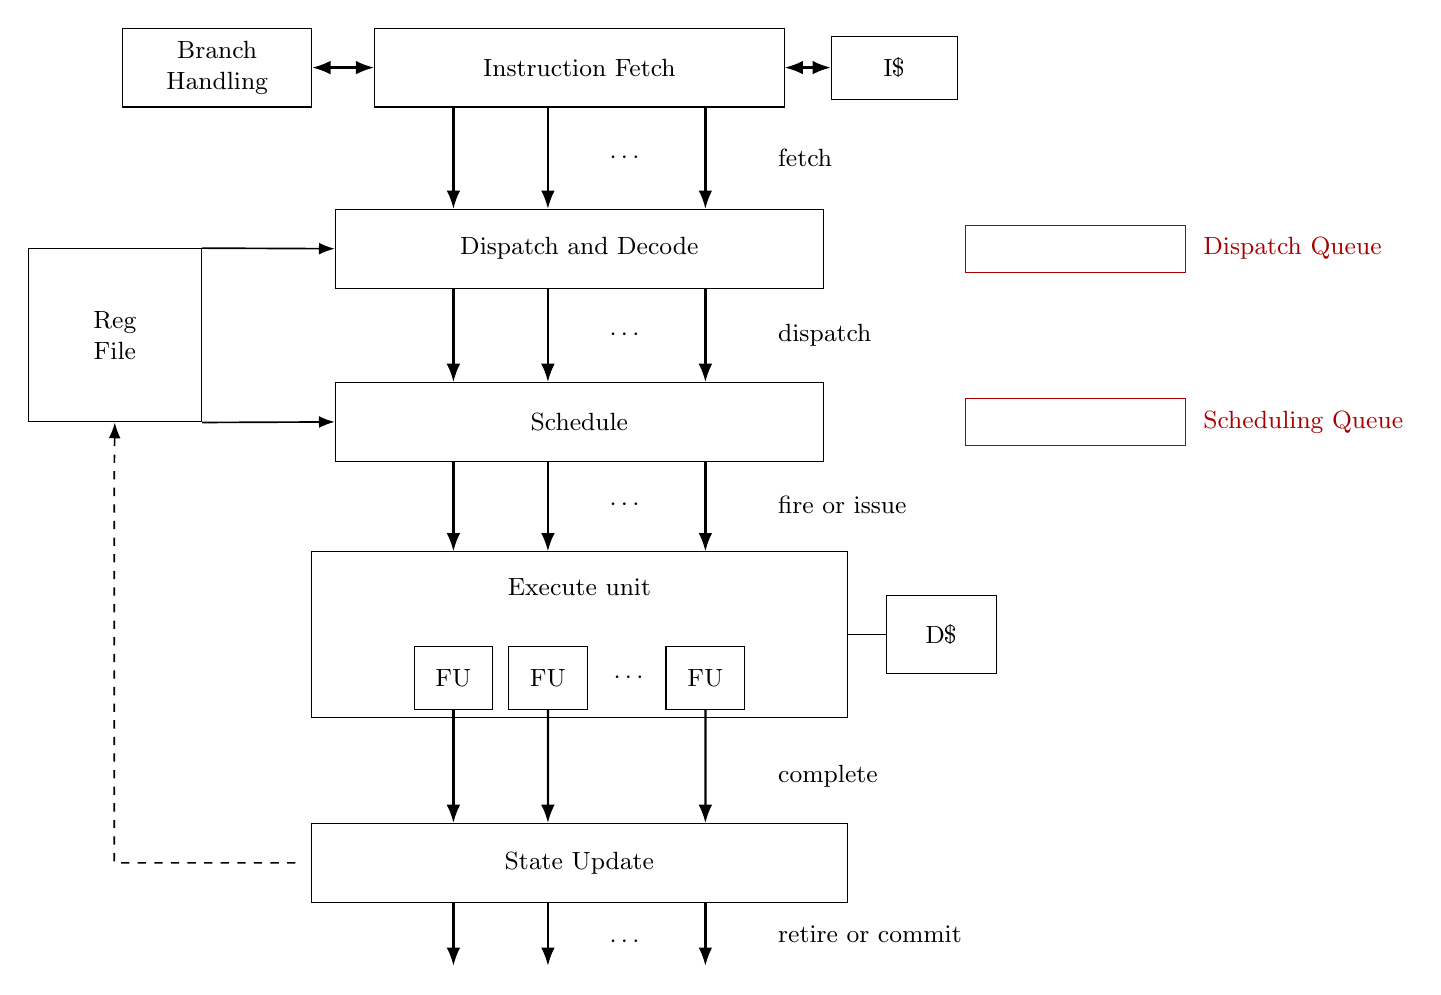
\begin{tikzpicture}[
        font=\small,
        >=Latex,
        box/.style={draw, rectangle, minimum height=10mm, minimum width=34mm, align=center},
        smallbox/.style={draw, rectangle, minimum height=8mm, minimum width=16mm, align=center},
        queue/.style={draw, rectangle, minimum height=6mm, minimum width=28mm, draw=red!65!black},
        stagearrow/.style={->, thick},
        sidearrow/.style={->, semithick},
        dasharrow/.style={->, dashed, semithick}
    ]

    % Top row
    \node[box, minimum width=24mm] (branch) at (0,0) {Branch\\Handling};
    \node[box, minimum width=52mm] (fetch) at (4.6,0) {Instruction Fetch};
    \node[smallbox] (icache) at (8.6,0) {I\$};

    % Main pipeline
    \node[box, minimum width=62mm] (dispatch) at (4.6,-2.3) {Dispatch and Decode};
    \node[box, minimum width=62mm] (schedule) at (4.6,-4.5) {Schedule};
    \node[box, minimum width=68mm, minimum height=21mm] (execute) at (4.6,-7.2) {};
    \node[box, minimum width=68mm] (state) at (4.6,-10.1) {State Update};
    \node at ($(execute.north)+(0,-0.45)$) {Execute unit};

    % Functional units inside execute
    \node[smallbox, minimum width=10mm, minimum height=8mm] (fu1) at (3.0,-7.75) {FU};
    \node[smallbox, minimum width=10mm, minimum height=8mm] (fu2) at (4.2,-7.75) {FU};
    \node at (5.25,-7.75) {$\cdots$};
    \node[smallbox, minimum width=10mm, minimum height=8mm] (fu3) at (6.2,-7.75) {FU};

    % Side structures
    \node[box, minimum width=22mm, minimum height=22mm] (regfile) at (-1.3,-3.4) {Reg\\File};
    \node[smallbox, minimum width=14mm, minimum height=10mm] (dcache) at (9.2,-7.2) {D\$};

    % Queues on right
    \node[queue] (dqueue) at (10.9,-2.3) {};
    \node[queue] (squeue) at (10.9,-4.5) {};

    % Connections at top
    \draw[<->, thick] (branch.east) -- (fetch.west);
    \draw[<->, thick] (fetch.east) -- (icache.west);

    % Vertical flow
    \draw[stagearrow] ($(fetch.south)+(-1.6,0)$) -- ($(dispatch.north)+(-1.6,0)$);
    \draw[stagearrow] ($(fetch.south)+(-0.4,0)$) -- ($(dispatch.north)+(-0.4,0)$);
    \draw[stagearrow] ($(fetch.south)+(1.6,0)$) -- ($(dispatch.north)+(1.6,0)$);
    \node at (5.2,-1.15) {$\cdots$};

    \draw[stagearrow] ($(dispatch.south)+(-1.6,0)$) -- ($(schedule.north)+(-1.6,0)$);
    \draw[stagearrow] ($(dispatch.south)+(-0.4,0)$) -- ($(schedule.north)+(-0.4,0)$);
    \draw[stagearrow] ($(dispatch.south)+(1.6,0)$) -- ($(schedule.north)+(1.6,0)$);
    \node at (5.2,-3.4) {$\cdots$};

    \draw[stagearrow] ($(schedule.south)+(-1.6,0)$) -- ($(execute.north)+(-1.6,0)$);
    \draw[stagearrow] ($(schedule.south)+(-0.4,0)$) -- ($(execute.north)+(-0.4,0)$);
    \draw[stagearrow] ($(schedule.south)+(1.6,0)$) -- ($(execute.north)+(1.6,0)$);
    \node at (5.2,-5.55) {$\cdots$};

    \draw[stagearrow] (fu1.south) -- ($(state.north)+(-1.6,0)$);
    \draw[stagearrow] (fu2.south) -- ($(state.north)+(-0.4,0)$);
    \draw[stagearrow] (fu3.south) -- ($(state.north)+(1.6,0)$);

    \draw[stagearrow] ($(state.south)+(-1.6,0)$) -- ++(0,-0.8);
    \draw[stagearrow] ($(state.south)+(-0.4,0)$) -- ++(0,-0.8);
    \draw[stagearrow] ($(state.south)+(1.6,0)$) -- ++(0,-0.8);
    \node at (5.2,-11.10) {$\cdots$};

    % Left-side register file connections
    \draw[sidearrow] (regfile.north east) -- ($(dispatch.west)+(0,0.00)$);
    \draw[sidearrow] (regfile.south east) -- ($(schedule.west)+(0,0.00)$);
    \draw[dasharrow] ($(state.west)+(-0.2,0)$) -- ++(-2.3,0) -- ++(0,5.0) -- (regfile.south);

    % D-cache connection
    \draw[-, semithick] (execute.east) -- (dcache.west);

    % Labels on right
    \node[anchor=west] at (7.0,-1.15) {fetch};
    \node[anchor=west, text=red!65!black] at (12.4,-2.3) {Dispatch Queue};
    \node[anchor=west] at (7.0,-3.4) {dispatch};
    \node[anchor=west, text=red!65!black] at (12.4,-4.5) {Scheduling Queue};
    \node[anchor=west] at (7.0,-5.55) {fire or issue};
    \node[anchor=west] at (7.0,-9.0) {complete};
    \node[anchor=west] at (7.0,-11.0) {retire or commit};

    \end{tikzpicture}
    \caption{Generic logical superscalar pipeline view illustrating one possible organization. It is not itself specific to FICI, FICO, or FOCO; those classifications depend on how firing and completion are implemented. Boxed elements denote the main structures or stages, while the right-side annotations denote the adjacent flow actions: fetch, dispatch, fire or issue, complete, and retire or commit. Representative side structures and queues are also shown.}
    \label{fig:ilp-superscalar-pipeline}
\end{figure}


\section{Dependency Types and Why They Matter}\label{sec:ilp-dependencies}
Superscalar scheduling must respect three dependency classes.
\begin{itemize}
    \item \textit{RAW} (read-after-write) is a true flow dependency.
    A later instruction needs a value produced by an earlier one, so executing them in the wrong order would use stale data and produce the wrong result.
    \item \textit{WAR} (write-after-read) is an anti-dependency.
    A later instruction must not overwrite a register before an earlier instruction has finished reading it, even though the two instructions do not share a true data value.
    \item \textit{WAW} (write-after-write) is an output dependency.
    Two instructions write the same destination, so their writes must appear in the correct order or the final architectural value will be wrong.
\end{itemize}
Only RAW is fundamentally unavoidable.
WAR and WAW are name dependencies that arise from register reuse and can be reduced or removed by renaming the register.


\section{Fire/Complete Taxonomy}\label{sec:ilp-fire-complete}
A compact way to classify designs is by fire order and complete order.
\begin{itemize}
    \item \textit{FICI}: fire in order, complete in order (classic simple pipeline behavior).
    Instructions begin execution in program order and also finish in program order, which simplifies control but limits how much parallelism the machine can exploit.
    \item \textit{FICO}: fire in order, complete out of order (simpler superscalar step).
    Instructions still begin execution in order, but different latencies allow later instructions to finish first, so some parallel speedup is possible without fully out-of-order scheduling.
    \item \textit{FOCO}: fire out of order, complete out of order (more aggressive and higher potential ILP).
    The scheduler may start and finish instructions whenever operands and hardware are ready, which exposes more ILP but requires more machinery to preserve correct architectural behavior.
\end{itemize}


\section{Scoreboarding Intuition (FICO Style)}\label{sec:ilp-scoreboard}
A scoreboard tracks whether sources, destinations, and required function units are currently available.
A simplified FICO-style fire condition is shown in Eq.~\eqref{eq:ilp-fire-condition}.
\begin{equation}\label{eq:ilp-fire-condition}
    \text{Fire if }\neg busy(src_1)\ \wedge\ \neg busy(src_2)\ \wedge\ \neg busy(dest)\ \wedge\ \neg busy(FU_{needed}).
\end{equation}
When an instruction fires, destination and function-unit busy state are set.
When the instruction completes, those busy states are cleared according to implementation timing rules.
The result is correct execution with modest hardware complexity, but some parallel opportunities are still left unused compared with more aggressive out-of-order firing.


\section{Function Units and Latency}\label{sec:ilp-latency}
Superscalar benefit depends on latency balance and available unit count.
Common assumptions are short ALU latency, longer multiply latency, and memory latency that depends heavily on cache behavior.
Designers therefore optimize both unit availability and scheduling policy, not just raw clock frequency.


\section{Register Renaming as the Next Step}\label{sec:ilp-renaming}
Renaming introduces additional physical register identities so later writes do not falsely block earlier reads or writes.
Conceptually, renaming transforms many WAR/WAW hazards into non-hazards while preserving program meaning.
The dependency pressure that remains is primarily RAW, which reflects true data flow.


\section{Speculation Without and With Prediction}\label{sec:ilp-speculation}
Superscalar pipelines use speculation to keep FUs busy.
Some designs can speculate without high-quality prediction (for example, eager execution ideas), but the useful work fraction is then limited.
High-accuracy branch handling usually gives better effective IPC because fewer speculative instructions are squashed.


\section{Chapter 6 Summary}\label{sec:chapter6-summary-ilp}
Instruction-level parallelism turns $CPI<1$ into a concrete microarchitectural target.
Superscalar design achieves this by widening the pipeline's effective throughput and managing dependencies, hazards, and speculative state carefully.
FICO-style scoreboarding illustrates the basic mechanism, while renaming and stronger out-of-order policies push performance further.
These ideas form the bridge from classic five-stage thinking to modern high-throughput scalar cores.

    \chapter[Compiler-Scheduled ILP]{Compiler-Scheduled ILP: VLIW and Software Pipelining}\label{ch:compiler-scheduled-ilp}

\section{VLIW as a Compiler-Scheduled Alternative}\label{sec:ilp-vliw}
One response to dynamic-scheduling complexity is to move more of the scheduling work into the compiler.
As superscalar windows grow, the machine would like a larger scheduling queue so it can search farther ahead for independent work, but larger queues also make wakeup, select, and operand-readiness checks harder to close at a short cycle time.
This leads to the \textit{very long instruction word (VLIW)} approach, historically associated with Josh Fisher.
A VLIW encoding packs several operations intended to execute in parallel into one instruction word, so the compiler decides the schedule at compile time rather than letting large runtime scheduling hardware discover it dynamically.

In this context, an individual encoded action is an \textit{op}.
A set of ops intended to execute in the same cycle is a \textit{multi-op}.
VLIW reduces runtime hardware complexity because the machine no longer needs a large associative scheduling queue, aggressive wakeup logic, or much of the dynamic issue machinery used in FOCO-style processors.
The tradeoff is that the compiler must do much more work up front, and the resulting code is less adaptive to runtime variation such as cache misses or changing branch behavior.
This tradeoff is attractive in domains such as \textit{digital signal processors (DSPs)}, where workloads are regular and low-power execution is important.

Compiler design must balance three competing goals: code quality, compilation time, and maintainability.
In practice, that usually rules out algorithms much worse than quadratic for large compiler passes, and even cubic methods are used cautiously.
In principle, finding the optimal schedule for a dependence-constrained block is exponential in block size, so practical VLIW compilers rely on heuristics rather than on exact search.
List scheduling is one of the standard heuristics for this job.
The broader performance point is that widening fetch and scheduling machinery yields diminishing returns: useful IPC usually grows sublinearly with front-end width, while the cost of dynamic scheduling hardware grows quickly.


\section{Dependence Graphs and List Scheduling}\label{sec:ilp-vliw-list-scheduling}
The compiler begins from a \textit{data dependence graph}.
True flow edges capture read-after-write dependencies, while anti-dependence and output-dependence edges capture false constraints caused by register reuse.
Pure flow dependence always takes priority over false dependence because it represents real data movement.
If the code contains loops, this graph can contain cycles, so it is not necessarily a directed acyclic graph.
Constructing the graph by hand is mechanical.
First draw one node per op.
Then add all true flow edges from each definition to the later uses that require that value.
Next add anti-dependence edges from a read to a later write of the same architectural name, and output-dependence edges between two writes of the same name.
If two operations are already ordered by a true flow dependence, that true edge is the one that matters for scheduling because it already enforces the required order.

Table~\ref{tab:ilp-vliw-block} gives a compact block that will be used for the scheduling example.
Assume one pipelined load/store unit, one pipelined arithmetic logic unit (ALU), and one pipelined multiplier.
Each unit can accept a new op every cycle; the listed latencies describe when results become available, not how long the unit remains occupied.
Also assume the compiler has already assigned registers so that the remaining constraints shown in the table are dominated by true dependences rather than by avoidable name conflicts.
\begin{table}[t]
    \centering
    \renewcommand{\arraystretch}{1.15}
    \begin{tabular}{|c|l|l|c|}
        \hline
        Instr.
        & Operation & True dependences & Latency \\
        \hline
        A & LW $R2, X$ & None & 2 \\
        \hline
        B & LW $R3, Y$ & None & 2 \\
        \hline
        C & LW $R4, Z$ & None & 2 \\
        \hline
        D & ADD $R5, R1, R2$ & A & 1 \\
        \hline
        E & MUL $R6, R2, R3$ & A, B & 3 \\
        \hline
        F & MUL $R7, R1, R3$ & B & 3 \\
        \hline
        G & ADD $R8, R7, \#1$ & F & 1 \\
        \hline
        H & SW $R8, X$ & G & 1 \\
        \hline
        I & ADD $R9, R2, R4$ & A, C & 1 \\
        \hline
    \end{tabular}
    \caption{Illustrative basic block for VLIW list scheduling.}
    \label{tab:ilp-vliw-block}
\end{table}
Figure~\ref{fig:ilp-vliw-ddg} presents the same block in a more visual form: the original operations, the resulting data dependence graph, and one priority list ordered by dependence height.
\begin{figure}[t]
    \centering
    \small
    \begin{minipage}[t]{0.27\textwidth}
        \raggedright
        \textbf{Original operations}\par
        \vspace{0.5ex}
        \begin{tabular}[t]{@{}ll@{}}
            A: & LW $R2, X$ \\
            B: & LW $R3, Y$ \\
            C: & LW $R4, Z$ \\
            D: & ADD $R5, R1, R2$ \\
            E: & MUL $R6, R2, R3$ \\
            F: & MUL $R7, R1, R3$ \\
            G: & ADD $R8, R7, \#1$ \\
            H: & SW $R8, X$ \\
            I: & ADD $R9, R2, R4$
        \end{tabular}
    \end{minipage}\hfill
    \begin{minipage}[t]{0.45\textwidth}
        \centering
        \textbf{Data Dependence Graph}\par
        \vspace{1ex}
        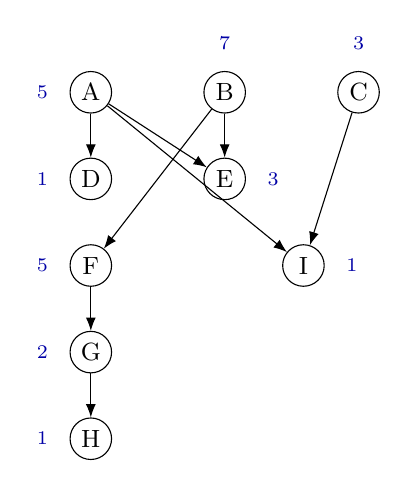
\begin{tikzpicture}[
            >=Latex,
            depnode/.style={draw, circle, inner sep=1pt, minimum size=15pt, font=\small},
            hlabel/.style={font=\scriptsize, text=blue!65!black}
        ]
            \node[depnode] (A) at (0,0) {A};
            \node[depnode] (B) at (1.7,0) {B};
            \node[depnode] (C) at (3.4,0) {C};
            \node[depnode] (D) at (0,-1.1) {D};
            \node[depnode] (E) at (1.7,-1.1) {E};
            \node[depnode] (F) at (0,-2.2) {F};
            \node[depnode] (I) at (2.7,-2.2) {I};
            \node[depnode] (G) at (0,-3.3) {G};
            \node[depnode] (H) at (0,-4.4) {H};

            \node[hlabel, left=1.5mm of A] {$5$};
            \node[hlabel, above=1.5mm of B] {$7$};
            \node[hlabel, above=1.5mm of C] {$3$};
            \node[hlabel, left=1.5mm of D] {$1$};
            \node[hlabel, right=1.5mm of E] {$3$};
            \node[hlabel, left=1.5mm of F] {$5$};
            \node[hlabel, right=1.5mm of I] {$1$};
            \node[hlabel, left=1.5mm of G] {$2$};
            \node[hlabel, left=1.5mm of H] {$1$};

            \draw[->] (A) -- (D);
            \draw[->] (A) -- (E);
            \draw[->] (A) -- (I);
            \draw[->] (B) -- (E);
            \draw[->] (B) -- (F);
            \draw[->] (C) -- (I);
            \draw[->] (F) -- (G);
            \draw[->] (G) -- (H);
        \end{tikzpicture}
    \end{minipage}\hfill
    \begin{minipage}[t]{0.20\textwidth}
        \raggedright
        \textbf{List ordered by dependence height}\par
        \vspace{0.5ex}
        \begin{tabular}[t]{@{}l@{}}
            $B$ $(7)$ \\
            $A$ $(5)$ \\
            $F$ $(5)$ \\
            $C$ $(3)$ \\
            $E$ $(3)$ \\
            $G$ $(2)$ \\
            $D$ $(1)$ \\
            $I$ $(1)$ \\
            $H$ $(1)$
        \end{tabular}
    \end{minipage}
    \caption{Original operations, dependence graph, and one priority ordering for the VLIW list-scheduling example. The small numeric annotations next to nodes indicate dependence height. Ties may be broken arbitrarily.}
    \label{fig:ilp-vliw-ddg}
\end{figure}

One common priority heuristic is \textit{dependence height}, which estimates how much latency remains below a node on the longest dependent path.
If the heuristic includes the latency of the current instruction itself, one convenient definition is Eq.~\eqref{eq:ilp-dependence-height}.
\begin{equation}\label{eq:ilp-dependence-height}
    height(i)=
    \begin{cases}
        lat(i), & succ(i)=\emptyset\\
        lat(i)+\max\limits_{j\in succ(i)} height(j), & \text{otherwise}
    \end{cases}
\end{equation}
Higher-height instructions receive higher priority because delaying them is more likely to lengthen the critical path.
To annotate a graph by hand, start from the sinks and assign each sink its own latency.
Then sweep backward, adding the current node latency to the maximum height among its successors.
The ready list is obtained by sorting nodes from highest height to lowest, breaking ties either arbitrarily or by an explicit secondary rule such as program order.
For the block in Table~\ref{tab:ilp-vliw-block}, the longest true-dependence chain is $B\rightarrow F\rightarrow G\rightarrow H$, so the heuristic tends to prioritize $F$ ahead of $E$ once both become candidates for the single multiplier.

List scheduling then tries to place the highest-priority ready instructions into each cycle subject to both dependence timing and resource availability.
A simple legality condition is shown in Eq.~\eqref{eq:ilp-list-schedule-legal}.
\begin{equation}\label{eq:ilp-list-schedule-legal}
    cycle(i)=\min\!\left\{c\ \middle|\ \forall j\in pred(i),\ c\ge cycle(j)+lat(j),\ \text{and a compatible FU is free in }c \right\}.
\end{equation}
This is not an optimal algorithm, but it is practical and captures the central VLIW idea: schedule as much parallel work as possible before runtime while still respecting dependencies and resource limits.

Table~\ref{tab:ilp-vliw-schedule} shows one possible compiler-produced schedule for the block running on a machine with one arithmetic logic unit (ALU), one multiplier, and one load/store unit.
The point is not that this schedule is unique, but that the compiler can decide the cycle packing in advance and encode it directly.
For illustration, this schedule keeps the three initial loads in source order even though a greedier dependence-height policy could start $B$ before $A$ and shorten the block by one cycle.
That choice leaves one explicit empty cycle later, which makes the pause-field encoding example concrete.
\begin{table}[t]
    \centering
    \renewcommand{\arraystretch}{1.15}
    \begin{tabular}{|c|c|c|c|}
        \hline
        Cycle & Load/Store Unit & ALU & Multiplier \\
        \hline
        1 & A &  &  \\
        \hline
        2 & B &  &  \\
        \hline
        3 & C & D &  \\
        \hline
        4 &  &  & F \\
        \hline
        5 &  & I & E \\
        \hline
        6 &  &  &  \\
        \hline
        7 &  & G &  \\
        \hline
        8 & H &  &  \\
        \hline
    \end{tabular}
    \caption{One legal VLIW-style schedule for the block under fixed functional-unit limits.}
    \label{tab:ilp-vliw-schedule}
\end{table}
The schedule shows two important points.
First, the compiler only packs operations together when both the dependence constraints and the functional-unit constraints allow it.
Second, the absence of an operation in a slot does not require the hardware to discover what to do; the compiler can encode the schedule directly.
In particular, cycle 6 is intentionally empty because $G$ cannot start until the three-cycle multiply $F$ has finished producing $R7$.
Table~\ref{tab:ilp-vliw-packed-schedule} shows the same schedule in a field-level packing format closer to an actual multi-op layout.
This table defines which operands occupy each unit's fields in each cycle; it does not by itself define the serialized op order in memory.
\begin{table}[t]
    \centering
    \small
    \setlength{\tabcolsep}{4pt}
    \renewcommand{\arraystretch}{1.12}
    \begin{tabular}{|c|c c c|c c c|c c|c c|}
        \hline
        Cycle & \multicolumn{3}{c|}{IALU (1 cycle)} & \multicolumn{3}{c|}{MUL (3 cycles)} & \multicolumn{2}{c|}{Load (2 cycles)} & \multicolumn{2}{c|}{Store (1 cycle)} \\
        \hline
         & $d$ & $s_1$ & $s_2$ & $d$ & $s_1$ & $s_2$ & $d$ & addr & addr & $s$ \\
        \hline
        1 &  &  &  &  &  &  & $R2$ & $X$ &  &  \\
        \hline
        2 &  &  &  &  &  &  & $R3$ & $Y$ &  &  \\
        \hline
        3 & $R5$ & $R1$ & $R2$ &  &  &  & $R4$ & $Z$ &  &  \\
        \hline
        4 &  &  &  & $R7$ & $R1$ & $R3$ &  &  &  &  \\
        \hline
        5 & $R9$ & $R2$ & $R4$ & $R6$ & $R2$ & $R3$ &  &  &  &  \\
        \hline
        6 &  &  &  &  &  &  &  &  &  &  \\
        \hline
        7 & $R8$ & $R7$ & $\#1$ &  &  &  &  &  &  &  \\
        \hline
        8 &  &  &  &  &  &  &  &  & $X$ & $R8$ \\
        \hline
    \end{tabular}
    \caption{Field-level packing of the schedule from Table~\ref{tab:ilp-vliw-schedule}. Rows 3 and 5 are multi-ops because they contain more than one op in the same cycle.}
    \label{tab:ilp-vliw-packed-schedule}
\end{table}


\section{Multi-Op Encoding, Tail Bits, and Pause Fields}\label{sec:ilp-vliw-encoding}
VLIW raises an encoding question: how should a machine represent the boundaries of a multi-op if not every cycle uses every functional unit?
One simple approach is to fill every unused slot with an explicit no-op, but that wastes code space.
An alternative is to encode only real ops and add a small amount of grouping information.
Each encoded op still carries its ordinary fields such as opcode, destination register, and source registers; the additional VLIW-specific fields only describe grouping and delay.

One useful scheme adds a \textit{tail bit} to each encoded op.
If the tail bit is 0, the current op is not the end of the current multi-op.
If the tail bit is 1, the current op ends the current multi-op.
The next op then begins a new multi-op.
This lets the instruction stream represent a variable number of ops per cycle without requiring every cycle to contain the same number of explicit no-op fillers.

A related field is a \textit{pause field}, which tells the front-end control logic to wait a specified number of cycles before beginning the next multi-op.
In the simple scheme used here, the pause value is interpreted only on the op whose tail bit ends the current multi-op; pause values on earlier ops in the same multi-op are ignored.
This is a compact way to represent silence between multi-ops while still keeping each op's encoding regular.
Table~\ref{tab:ilp-vliw-encoding} illustrates the idea using the schedule from Table~\ref{tab:ilp-vliw-schedule}.
It shows one legal serialized op order for the same multi-ops that appear in Table~\ref{tab:ilp-vliw-packed-schedule}.
\begin{table}[t]
    \centering
    \renewcommand{\arraystretch}{1.15}
    \begin{tabular}{|c|c|c|p{2.9in}|}
        \hline
        Encoded op & Tail & Pause & Meaning \\
        \hline
        A & 1 & 0 & Single-op multi-op for cycle 1. \\
        \hline
        B & 1 & 0 & Single-op multi-op for cycle 2. \\
        \hline
        C & 0 & 0 & First op of the cycle-3 multi-op. \\
        \hline
        D & 1 & 0 & Ends the cycle-3 multi-op. \\
        \hline
        F & 1 & 0 & Single-op multi-op for cycle 4. \\
        \hline
        I & 0 & 0 & First op of the cycle-5 multi-op. \\
        \hline
        E & 1 & 1 & Ends the cycle-5 multi-op and inserts one pause cycle before the next multi-op. \\
        \hline
        G & 1 & 0 & Single-op multi-op for cycle 7. \\
        \hline
        H & 1 & 0 & Single-op multi-op for cycle 8. \\
        \hline
    \end{tabular}
    \caption{Illustrative VLIW encoding using tail bits and a pause field rather than explicit no-op padding.}
    \label{tab:ilp-vliw-encoding}
\end{table}
Some implementations instead use simple interlocking at the multi-op level, which can remove the need for an explicit pause field.
That saves encoding space, but it also gives up some of the compiler's direct control over exactly when the next multi-op may begin.


\section{Software Pipelining and Cyclic Scheduling}\label{sec:ilp-software-pipelining}
Loops create another opportunity for compiler-scheduled parallelism.
Instead of scheduling only one copy of a loop body, the compiler can overlap operations from different iterations so that a later iteration begins before an earlier one has fully finished.
The older name for this idea is \textit{polycyclic scheduling}; the more common modern name is \textit{software pipelining}.

Conceptually, the compiler behaves as if it had unrolled the loop many times, compacted the overlapping schedule, and then kept only the repeating pattern.
That repeating pattern is the \textit{kernel}.
The code that fills the pipeline before the kernel reaches steady state is the \textit{prologue}.
The code that drains the remaining work after loop exit is the \textit{epilogue}.
The distance in cycles between the start of successive iterations is the \textit{initiation interval (II)}.
Once the schedule reaches steady state, the loop begins a new iteration every $II$ cycles, so the throughput is $1/II$ iterations per cycle.


\section{Iterative Modulo Scheduling}\label{sec:ilp-iterative-modulo-scheduling}
A practical way to construct such schedules is \textit{Iterative Modulo Scheduling (IMS)}.
The compiler first estimates a lower bound on $II$, then attempts to build a modulo schedule at that value.
If the attempt fails, it increments $II$ and tries again.

The first bound comes from resource pressure.
If a loop contains $N_t$ operations of type $t$ and the machine provides $U_t$ compatible units of that type, then
\begin{equation}\label{eq:ilp-res-ii}
    ResII=\max_t \left\lceil \frac{N_t}{U_t} \right\rceil
\end{equation}
This is the resource-constrained initiation interval.

The second bound comes from loop-carried recurrences.
If a dependence cycle $c$ has total latency $Lat(c)$ and spans $Dist(c)$ loop iterations, then
\begin{equation}\label{eq:ilp-rec-ii}
    RecII=\max_c \left\lceil \frac{Lat(c)}{Dist(c)} \right\rceil
\end{equation}
This is the recurrence-constrained initiation interval.
If the dependence graph has no loop-carried cycles, then the practical lower bound is $RecII=1$.

The schedule must satisfy both limits, so the compiler begins from
\begin{equation}\label{eq:ilp-min-ii}
    MII=\max(ResII,RecII),\qquad II\ge MII.
\end{equation}
Many texts call this lower bound the \textit{minimum initiation interval (MII)}.
IMS therefore follows a simple pattern:
\begin{enumerate}
    \item Start with $II=MII$.
    \item Attempt a legal modulo schedule at that value.
    \item If the attempt fails, increment $II$ and retry.
\end{enumerate}
A modulo reservation table for a chosen $II$ has exactly $II$ rows.
An operation that would occupy cycle $x$ in a longer unrolled schedule is placed into row $x \bmod II$, provided the dependence and resource constraints remain legal.

In most textbook treatments, the underlying machine is modeled with a point-latency abstraction: an op occupies one issue slot, then its result becomes ready after a fixed latency.
This keeps the scheduling problem manageable.
More detailed models that explicitly schedule register-file ports, result buses, and intermediate pipeline stages are possible, but they are much more expensive to optimize and are usually avoided in introductory treatments.


\section{Worked Software-Pipelining Example}\label{sec:ilp-software-pipelining-example}
Table~\ref{tab:ilp-swpipe-loop} shows a small loop that illustrates the idea.
Assume two arithmetic logic units, two memory units, one-cycle add/branch latency, and two-cycle load latency.
The branch still logically closes the loop body even though later iterations will overlap older ones.
\begin{table}[t]
    \centering
    \renewcommand{\arraystretch}{1.15}
    \begin{tabular}{|c|l|l|c|}
        \hline
        Instr.
        & Operation & Key dependences & Latency \\
        \hline
        A & ADD $R2, R2, \#1$ & loop-carried on $R2$ & 1 \\
        \hline
        B & LW $R3, 0(R2)$ & A & 2 \\
        \hline
        C & SW $R0, 0(R3)$ & B & 1 \\
        \hline
        D & ADD $R10, R10, \#1$ & loop-carried on $R10$ & 1 \\
        \hline
        E & BRGTZ $R10$, LOOP & D; branch must close the loop body & 1 \\
        \hline
    \end{tabular}
    \caption{Loop used to illustrate software pipelining and modulo scheduling.}
    \label{tab:ilp-swpipe-loop}
\end{table}

The cyclic dependence view of this loop contains the within-iteration edges $A_i\rightarrow B_i$, $B_i\rightarrow C_i$, and $D_i\rightarrow E_i$, plus the loop-carried edges $A_i\rightarrow A_{i+1}$ and $D_i\rightarrow D_{i+1}$.
Those loop-carried edges are exactly the recurrences used when computing $RecII$.

For this loop, the resource bound is
\[
ResII=\max\!\left(\left\lceil \frac{3\ \text{ALU/branch ops}}{2\ \text{ALUs}} \right\rceil,
\left\lceil \frac{2\ \text{memory ops}}{2\ \text{memory units}} \right\rceil \right)=\max(2,1)=2.
\]
The loop-carried recurrences on $R2$ and $R10$ each have latency 1 and distance 1, so $RecII=1$.
Therefore the first useful attempt is $II=2$.

One legal modulo reservation table is shown in Table~\ref{tab:ilp-swpipe-kernel}.
The first row begins iteration $i$.
The second row finishes the current iteration's control work while also performing the store from iteration $i-1$.
That overlap is the essence of software pipelining.
\begin{table}[t]
    \centering
    \renewcommand{\arraystretch}{1.15}
    \begin{tabular}{|c|c|c|c|c|}
        \hline
        Modulo slot & ALU 0 & ALU 1 & MEM 0 & MEM 1 \\
        \hline
        0 & $A_i$ & $D_i$ &  &  \\
        \hline
        1 & $E_i$ &  & $B_i$ & $C_{i-1}$ \\
        \hline
    \end{tabular}
    \caption{One modulo reservation table for the loop in Table~\ref{tab:ilp-swpipe-loop} with $II=2$.}
    \label{tab:ilp-swpipe-kernel}
\end{table}

The emitted code must still handle loop entry and loop exit correctly.
Table~\ref{tab:ilp-swpipe-phases} separates the schedule into prologue, kernel, and epilogue form.
The early-exit branch $E^\ast$ is the inverted form of the loop branch; it lets the machine leave the prologue cleanly if the loop should terminate before the steady-state kernel is entered.
\begin{table}[t]
    \centering
    \renewcommand{\arraystretch}{1.15}
    \begin{tabular}{|c|l|}
        \hline
        Phase & Operations \\
        \hline
        Prologue & $A_1, D_1$ \quad then \quad $B_1, E^\ast_1$ \\
        \hline
        Kernel & repeat every $II=2$ cycles: \quad $A_i, D_i$ \quad then \quad $B_i, C_{i-1}, E_i$ \\
        \hline
        Epilogue & $C_{\text{last}}$ \\
        \hline
    \end{tabular}
    \caption{Prologue, kernel, and epilogue for the software-pipelined loop.}
    \label{tab:ilp-swpipe-phases}
\end{table}

This example also shows why software pipelining is attractive for VLIW machines.
The compiler exposes the repeating parallel structure explicitly, so the hardware can execute the steady-state kernel with very little dynamic scheduling logic.
At the same time, general-purpose superscalar machines still benefit from dynamic scheduling because real loads do not always return in a fixed number of cycles and binaries may need to run across several microarchitectural variants.


\section{Memory Disambiguation}\label{sec:ilp-vliw-memory-disambiguation}
Loads and stores create a special scheduling problem.
If a compiler moves a load ahead of an older store to the same address, the load may read the wrong value.
The compiler therefore needs \textit{memory disambiguation}: it must prove that two memory references do not overlap, or else it must preserve the original order or insert explicit synchronization.

This is one of the limits of VLIW compared with dynamic scheduling hardware.
An out-of-order processor may speculate and recover if it guesses wrong.
A VLIW compiler must usually be more conservative unless it has strong alias information.
That is one reason VLIW works best when memory behavior is regular enough for compile-time reasoning to be reliable.

\section{Chapter 7 Summary}\label{sec:chapter7-summary-vliw}
Compiler-scheduled ILP takes a different approach from dynamic superscalar scheduling.
Instead of building increasingly complex runtime issue logic, a VLIW machine relies on the compiler to expose parallel ops ahead of time and encode them explicitly.
Data dependence graphs, dependence-height ordering, and list scheduling provide the basic machinery for building legal multi-ops.
Tail-bit and pause-field encoding then translate that schedule into a compact instruction stream without filling unused slots with explicit no-ops.
Software pipelining extends the same idea across loop iterations by constructing a prologue, steady-state kernel, and epilogue around a chosen initiation interval.
Memory disambiguation remains the key correctness limit: compile-time scheduling can move loads and stores only when aliasing is understood well enough to preserve program behavior.
Together these techniques show how compiler scheduling can approach the performance of aggressive ILP hardware while trading hardware complexity for compile-time analysis.

    \chapter[Multiprocessor Fundamentals]{Multiprocessor Architecture Fundamentals: Shared Memory, Interconnects, and Cache Coherence}\label{ch:multiprocessors}


\section{From Instruction-Level to Thread-Level Parallelism}\label{sec:mp-intro}
Once a machine has already exploited as much instruction-level parallelism as is practical, the next major source of speedup is to execute more than one thread of control at the same time.
This moves the discussion from single-core scheduling into \textit{multiprocessor} design.
At this point the most visible form of parallelism is \textit{thread-level parallelism (TLP)}: the programmer or runtime system must decide how to divide work across multiple processing elements.
Unlike instruction-level parallelism, thread-level parallelism is visible to software and therefore directly affects correctness, synchronization, and programmability.

Historically, architecture texts often used the term \textit{processing element (PE)} for one independently executing processor in a larger machine.
Modern commercial systems more often use \textit{core}, but the older PE terminology remains useful because it applies equally well to CPUs, accelerator lanes, and other specialized execution agents.
Table~\ref{tab:mp-grain-size} places multiprocessors in the broader grain-size view of parallelism.
\begin{table}[!b]
    \centering
    \footnotesize
    \renewcommand{\arraystretch}{1.15}
    \begin{tabular}{|>{\raggedright\arraybackslash}p{1.15in}|>{\raggedright\arraybackslash}p{2.00in}|>{\raggedright\arraybackslash}p{1.55in}|}
        \hline
        Parallelism level & Typical mechanism                                 & Programmer visibility                            \\
        \hline
        Instruction-level & superscalar issue, out-of-order execution, VLIW   & usually hidden                                   \\
        \hline
        Data-level        & SIMD vectors, packed operations, vector pipelines & partly visible through data layout or intrinsics \\
        \hline
        Thread-level      & multiple threads or PEs executing concurrently    & directly visible                                 \\
        \hline
    \end{tabular}
    \caption{Common grain sizes of parallelism. Multiprocessor programming is primarily concerned with the thread level.}
    \label{tab:mp-grain-size}
\end{table}

At the architecture-classification level, two familiar Flynn terms continue to matter:
\textit{Single instruction, multiple data (SIMD)} machines apply the same operation to multiple data elements at once.
\textit{Multiple instruction, multiple data (MIMD)} machines allow different PEs to execute different instructions on different data at the same time.
Modern shared-memory multiprocessors are usually discussed as MIMD machines.
That does not exclude SIMD units inside each core; it only means that the overall machine permits several independently executing instruction streams.


\section{Memory Organization and System Structure}\label{sec:mp-memory-organization}
A multiprocessor can be classified along another axis besides SIMD versus MIMD: how the memory system is organized.
The two clean endpoints are \textit{shared memory} and \textit{message passing}.

In a \textit{shared-memory} machine, all PEs conceptually operate in one common address space.
A pointer value can identify the same logical object for every PE, and communication occurs when one PE writes data that another PE later reads.
This model is attractive because it is easy to think about, but it immediately raises the cache-coherence problem once private caches are introduced.

In a \textit{message-passing} machine, each PE has its own private memory, and data movement occurs through explicit communication operations such as \texttt{send()} and \texttt{receive()}.
This model avoids coherence traffic because data is copied intentionally from one memory to another, but it forces the program to expose that communication directly.
Between these extremes lies the \textit{partitioned global address space (PGAS)} idea, where a single address space exists but some portions are substantially more expensive to access than others.

Figure~\ref{fig:mp-standalone-vs-accelerator} contrasts two common organizations.
A standalone shared-memory multiprocessor integrates several PEs around a common memory system and runs the operating system and application code directly.
An accelerator organization instead separates a host processor from a specialized parallel engine; the host launches work on the accelerator and explicitly copies data to and from accelerator memory.
\begin{figure}[t]
    \centering
    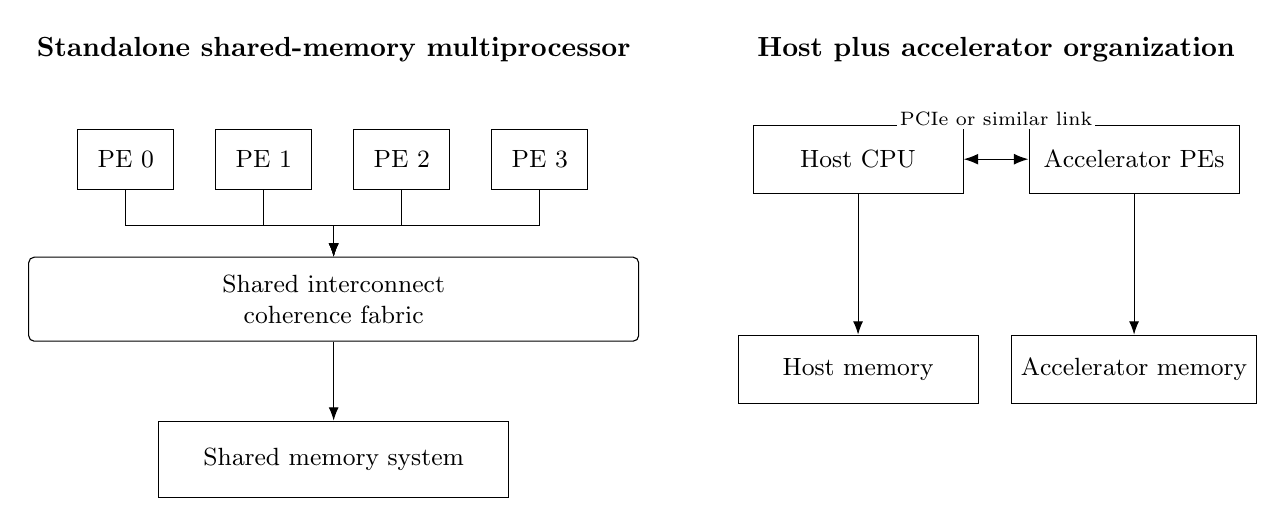
\begin{tikzpicture}[
        x=0.92in,
        y=1in,
        >=Latex,
        every node/.style={font=\small, align=center},
        pe/.style={draw, minimum width=0.48in, minimum height=0.30in},
        widebox/.style={draw, rounded corners=2pt, minimum height=0.42in, align=center},
        box/.style={draw, minimum width=1.05in, minimum height=0.34in, align=center},
        membox/.style={draw, minimum width=1.20in, minimum height=0.34in, align=center}
    ]
        \node[font=\bfseries] at (1.35,1.55) {Standalone shared-memory multiprocessor};
        \node[pe] (pe0) at (0.22,1.00) {PE 0};
        \node[pe] (pe1) at (0.97,1.00) {PE 1};
        \node[pe] (pe2) at (1.72,1.00) {PE 2};
        \node[pe] (pe3) at (2.47,1.00) {PE 3};
        \node[widebox, minimum width=3.05in] (ic) at (1.35,0.30) {Shared interconnect\\coherence fabric};
        \node[draw, minimum width=1.75in, minimum height=0.38in] (mem) at (1.35,-0.50) {Shared memory system};
        \foreach \n in {pe0,pe1,pe2,pe3} {
            \draw[->, line width=0.4pt] (\n.south) -- ++(0,-0.18) -| (ic.north);
        }
        \draw[->, line width=0.4pt] (ic.south) -- (mem.north);

        \node[font=\bfseries] at (4.95,1.55) {Host plus accelerator organization};
        \node[box] (cpu) at (4.20,1.00) {Host CPU};
        \node[box] (acc) at (5.70,1.00) {Accelerator PEs};
        \node[membox] (hmem) at (4.20,-0.05) {Host memory};
        \node[membox] (amem) at (5.70,-0.05) {Accelerator memory};
        \draw[<->, line width=0.5pt] (cpu.east) -- (acc.west);
        \node[font=\scriptsize, fill=white, inner sep=1pt] at (4.95,1.20) {PCIe or similar link};
        \draw[->, line width=0.4pt] (cpu.south) -- (hmem.north);
        \draw[->, line width=0.4pt] (acc.south) -- (amem.north);
    \end{tikzpicture}
    \caption{Two common multiprocessor organizations. Left: one shared-memory system. Right: a host plus accelerator with distinct memory, so software must move data explicitly.}
    \label{fig:mp-standalone-vs-accelerator}
\end{figure}

Accelerators include graphics processors, machine-learning accelerators, and many other specialized engines.
Their memories are often kept separate for protection, compatibility, and implementation reasons.
The cost of that separation is explicit data motion: the host must copy inputs to the accelerator, launch the parallel work, and copy results back.

\enlargethispage{2\baselineskip}


\section{Interconnects: Shared Buses and Point-to-Point Links}\label{sec:mp-interconnects}
The interconnect between PEs matters just as much as the PE count.
In this text, a \textit{bus} means a \textit{shared observable broadcast medium}: all agents attached to the bus can observe the transactions sent across it.
That observability is the key property used later by snooping coherence.

A \textit{point-to-point interconnect} behaves differently.
A packet is sent from one endpoint to another over a dedicated link, and unrelated agents do not automatically see that traffic.
Modern peripheral links such as \textit{PCI Express (PCIe)} fit this model even though informal conversation sometimes calls them buses.
PCIe uses differential pairs rather than one shared bundle of broadcast wires, so it scales better than a traditional shared bus but does not naturally support global observation of every memory transaction.

This distinction matters because some coherence mechanisms require every cache to observe every relevant request.
Snooping works naturally on a shared observable medium.
Directory-based coherence does not require broadcast visibility because a separate directory structure explicitly tracks who has each block.


\section{The Cache-Coherence Problem}\label{sec:mp-coherence-problem}
Shared memory becomes difficult as soon as each PE receives a private cache.
Without additional coordination, different caches can hold different copies of the same memory location and update them independently.
That breaks the programmer's illusion of one shared value.

Consider a memory location $x$ whose initial value is 1.
Assume three PEs each read $x$ and therefore bring a copy into their private caches.
Now suppose the following operations occur in program order:
\begin{enumerate}
    \item $P_0$ writes $x\leftarrow 22$.
    \item $P_1$ writes $x\leftarrow 44$.
    \item $P_2$ executes \texttt{x++}.
\end{enumerate}
If the caches do not coordinate, then $P_2$ may still read its stale local copy of 1, increment it, and write back 2.
The program order suggests that the increment should apply to the most recent visible value and therefore produce 45, but an incoherent cache system can easily produce 2 instead.
Table~\ref{tab:mp-incoherent-example} summarizes the failure.
\begin{table}[t]
    \centering
    \renewcommand{\arraystretch}{1.15}
    \begin{tabular}{|c|l|l|}
        \hline
        Step & Event                                                  & Locally visible value of $x$ \\
        \hline
        0    & Initial memory value                                   & memory holds 1               \\
        \hline
        1    & $P_0$, $P_1$, and $P_2$ all cache $x$                  & each cache now holds 1       \\
        \hline
        2    & $P_0$ writes $x\leftarrow 22$ in its cache             & $P_0$ sees 22                \\
        \hline
        3    & $P_1$ writes $x\leftarrow 44$ in its cache             & $P_1$ sees 44                \\
        \hline
        4    & $P_2$ executes \texttt{x++} using its stale cache copy & $P_2$ sees 2                 \\
        \hline
    \end{tabular}
    \caption{An incoherent-cache scenario. Each PE can observe a different value of the same logical variable.}
    \label{tab:mp-incoherent-example}
\end{table}

Simply using write-through caches does not solve the problem.
Write-through ensures that memory is updated promptly, but it does not inform the other caches that their local copies have become stale.
The real issue is not whether memory eventually receives the write; it is whether all cached copies remain mutually consistent.

A coherent cache system is normally expected to satisfy three properties:
\begin{enumerate}
    \item \textbf{Read-after-write semantics for one processor.} If a PE writes a value and no one else writes that location in the meantime, a later read by the same PE should return the value it wrote.
    \item \textbf{Eventual visibility to other processors.} If one PE writes a location and another PE later reads it, then after sufficient time has passed and assuming no intervening writes, the reader must eventually observe the value that was written.
    \item \textbf{Consistent ordering of writes.} All PEs must observe writes to the same location in a consistent causal order.
\end{enumerate}
The second property is intentionally phrased in terms of \textit{sufficient time} rather than instant propagation.
Physical systems cannot propagate signals across large chips or boards instantaneously.
Coherence therefore promises eventual agreement and a consistent write story, not instantaneous zero-time updates.


\section{Coherence Solution Families}\label{sec:mp-coherence-families}
Architecturally, there are three standard ways to solve the coherence problem.

The first is a \textit{shared-cache} design in which all PEs communicate through one common cache structure.
This avoids inter-cache inconsistency because there is only one place that holds the shared block state.
The weakness is scalability: once the shared cache becomes the bottleneck, adding more PEs does not produce linear speedup even for embarrassingly parallel workloads.

The second is \textit{directory-based coherence}.
A directory tracks which caches currently hold each block and coordinates invalidations, forwarded data, or ownership transfers.
This can scale better than a pure broadcast bus because the system does not require every cache to observe every request.

The third is \textit{snooping coherence}.
Here each cache has a \textit{snooper}: logic that knows both what is currently in that cache and what transactions are appearing on the shared interconnect.
If the interconnect is a shared observable medium, the snooper can react immediately when another PE requests a block that this cache currently owns or shares.
The remainder of this chapter develops the classic snooping approach because it exposes the central state-machine ideas clearly.


\section{Snooping Coherence and the MSI Protocol}\label{sec:mp-msi}
A classic starting point for snooping coherence is the \textit{MSI} protocol.
Each cached block is marked as \textit{modified (M)}, \textit{shared (S)}, or \textit{invalid (I)}.
The meaning of those states is summarized in Table~\ref{tab:mp-msi-state-meanings}.
\begin{table}[t]
    \centering
    \renewcommand{\arraystretch}{1.15}
    \begin{tabular}{|c|l|l|l|}
        \hline
        State & My copy                 & Other caches                      & Memory copy \\
        \hline
        M     & dirty and writable      & no one else has a valid copy      & stale       \\
        \hline
        S     & clean                   & others may also hold clean copies & correct     \\
        \hline
        I     & not valid in this cache & unspecified                       & unspecified \\
        \hline
    \end{tabular}
    \caption{Meaning of the three MSI states for one cache block.}
    \label{tab:mp-msi-state-meanings}
\end{table}

Two kinds of bus requests are especially important:
\begin{itemize}
    \item \texttt{GetS}: request shared read permission for a block.
    \item \texttt{GetM}: request exclusive access with intent to write.
\end{itemize}
A dirty eviction produces a \texttt{WriteBack} transaction.
Snoopers may also perform two high-level actions:
\begin{itemize}
    \item \textit{abort}: tell the requester to wait or retry because another cache still owns the necessary data or permission.
    \item \textit{intervene}: supply the data directly rather than letting memory respond.
\end{itemize}
Table~\ref{tab:mp-msi-bus-actions} summarizes the basic bus-level vocabulary.
\begin{table}[t]
    \centering
    \renewcommand{\arraystretch}{1.15}
    \begin{tabular}{|l|p{4.2in}|}
        \hline
        Transaction or action & Meaning                                                                         \\
        \hline
        \texttt{GetS}         & Read miss requesting a clean shared copy.                                       \\
        \hline
        \texttt{GetM}         & Read-for-ownership requesting exclusive writable access.                        \\
        \hline
        \texttt{WriteBack}    & Dirty block is written back to memory on eviction or ownership handoff.         \\
        \hline
        abort                 & Requester must wait or retry because another cache is still handling the block. \\
        \hline
        intervene             & A snooping cache supplies the current data value directly.                      \\
        \hline
    \end{tabular}
    \caption{Common bus transactions and snooper responses in a snooping MSI system.}
    \label{tab:mp-msi-bus-actions}
\end{table}

From the requesting PE's perspective, the stable-state behavior is simple.
If a block is invalid and the PE reads it, the cache issues \texttt{GetS} and moves to \texttt{S} when the data arrives.
If a block is invalid and the PE writes it, the cache issues \texttt{GetM} and moves to \texttt{M} when ownership arrives.
If a block is already shared and the PE wants to write, the cache must first upgrade through \texttt{GetM} so that all other copies are invalidated.
Table~\ref{tab:mp-msi-requester} gives one compact summary.
\begin{table}[t]
    \centering
    \renewcommand{\arraystretch}{1.15}
    \begin{tabular}{|c|l|l|l|}
        \hline
        Current state & Local event & Bus action         & Next state \\
        \hline
        I             & read miss   & \texttt{GetS}      & S          \\
        \hline
        I             & write miss  & \texttt{GetM}      & M          \\
        \hline
        S             & read hit    & none               & S          \\
        \hline
        S             & write hit   & \texttt{GetM}      & M          \\
        \hline
        M             & read hit    & none               & M          \\
        \hline
        M             & write hit   & none               & M          \\
        \hline
        S             & replacement & none               & I          \\
        \hline
        M             & replacement & \texttt{WriteBack} & I          \\
        \hline
    \end{tabular}
    \caption{Stable-state MSI behavior from the requesting cache's perspective.}
    \label{tab:mp-msi-requester}
\end{table}

From the snooper's perspective, the same bus requests mean something different.
If a cache in state \texttt{S} sees another PE request \texttt{GetM}, it must invalidate its own copy and move to \texttt{I}.
If a cache in state \texttt{M} sees \texttt{GetS}, it must ensure that the most recent data becomes visible and then downgrade to \texttt{S}.
If it sees \texttt{GetM} while in \texttt{M}, it must give up ownership entirely and move to \texttt{I}.
Table~\ref{tab:mp-msi-snooper} summarizes the stable-state snooping behavior.
\begin{table}[t]
    \centering
    \renewcommand{\arraystretch}{1.15}
    \begin{tabular}{|c|l|l|l|}
        \hline
        Current state & Snooped event                       & Action                                 & Next state \\
        \hline
        I             & sees \texttt{GetS} or \texttt{GetM} & none                                   & I          \\
        \hline
        S             & sees \texttt{GetS}                  & none                                   & S          \\
        \hline
        S             & sees \texttt{GetM}                  & invalidate local copy                  & I          \\
        \hline
        M             & sees \texttt{GetS}                  & provide or write back data, downgrade  & S          \\
        \hline
        M             & sees \texttt{GetM}                  & provide or write back data, invalidate & I          \\
        \hline
    \end{tabular}
    \caption{Stable-state MSI behavior from the snooper's perspective.}
    \label{tab:mp-msi-snooper}
\end{table}


\section{Transient States and a Worked Two-Cache Trace}\label{sec:mp-msi-trace}
Real buses and coherence fabrics are not instantaneous, so caches often need \textit{transient states} while waiting for a request to complete.
A common notation concatenates the path of the transition.
For example, \texttt{IM} means that the cache started in \texttt{I}, issued a request whose destination is \texttt{M}, and is still waiting for that request to complete.
Likewise, \texttt{SM} means a shared block has requested an upgrade to modified state but has not yet received final ownership.

Table~\ref{tab:mp-msi-trace} walks through a short two-cache scenario that mirrors the classic classroom introduction to MSI:
\begin{enumerate}
    \item $P_1$ has a read miss and obtains a shared copy.
    \item $P_2$ then has a read miss and also obtains a shared copy.
    \item $P_1$ writes the block and upgrades from \texttt{S} to \texttt{M}.
    \item $P_2$ then tries to write the same block, initially receives an abort, enters transient state \texttt{IM}, and retries after $P_1$ writes back or hands off the dirty value.
\end{enumerate}
\begin{table}[t]
    \centering
    \footnotesize
    \renewcommand{\arraystretch}{1.15}
    \begin{tabular}{|c|>{\raggedright\arraybackslash}p{1.15in}|>{\raggedright\arraybackslash}p{0.95in}|>{\raggedright\arraybackslash}p{1.25in}|>{\raggedright\arraybackslash}p{1.65in}|}
        \hline
        Step & Event                                   & Bus msg.\             & $P_1$ state or action                                                          & $P_2$ state or action                  \\
        \hline
        1    & $P_1$ read miss                         & \texttt{GetS}        & $I\rightarrow S$                                                               & $I\rightarrow I$                       \\
        \hline
        2    & $P_2$ read miss                         & \texttt{GetS}        & $S\rightarrow S$                                                               & $I\rightarrow S$                       \\
        \hline
        3    & $P_1$ write hit on shared block         & \texttt{GetM}        & $S\rightarrow M$                                                               & snoops \texttt{GetM}: $S\rightarrow I$ \\
        \hline
        4    & $P_2$ write miss while $P_1$ owns block & \texttt{GetM}, abort & snoops \texttt{GetM}: $M\rightarrow I$ with \texttt{WriteBack} or intervention & $I\rightarrow IM$ \\
        \hline
        5    & $P_2$ retries after ownership transfer  & retry \texttt{GetM}  & $I\rightarrow I$                                                               & $IM\rightarrow M$                      \\
        \hline
    \end{tabular}
    \caption{One worked MSI trace showing stable states, a transient \texttt{IM} state, and a write-ownership transfer between two caches.}
    \label{tab:mp-msi-trace}
\end{table}

The important insight is that the coherence protocol is maintaining one simple invariant: a writable dirty copy must be unique.
Whenever one cache acquires \texttt{M}, all competing copies must either become invalid or be updated into a clean shared form before execution continues.


\section{MESI, MOESI, and MOESIF Refinements}\label{sec:mp-mesi-moesi}
MSI captures the essential coherence idea, but practical protocols often add extra stable states that reduce unnecessary traffic.
The most common additions are \textit{exclusive (E)}, \textit{owned (O)}, and \textit{forward (F)}.
These states do not change the basic correctness goal.
They refine who may write, whether memory already has the current value, and which cache should respond to later requests.

\subsection*{Exclusive State and the Hit Line}
The \texttt{E} state means that one cache has the block, the block is clean, memory is correct, and no other cache currently holds a copy.
Its main advantage is that a later local write can move silently from \texttt{E} to \texttt{M} without first broadcasting \texttt{GetM}.
That saves an upgrade transaction when a PE reads a block and then soon writes it.

The system needs some way to determine whether the requester is truly the only cache holding the block.
In a snooping bus, a common mechanism is a \textit{hit line}: when a cache issues \texttt{GetS}, any other cache that already has the block asserts one shared indication line.
If no cache asserts the line, the requester may enter \texttt{E}; otherwise it must enter \texttt{S}.
Without that shared-presence indication, the protocol cannot safely distinguish ``only clean copy'' from ``one of several clean copies.''

\subsection*{Owned and Forward States}
The \texttt{O} and \texttt{F} states refine what happens after a cache-to-cache transfer.
Suppose a cache holds a dirty block in \texttt{M} and another PE requests \texttt{GetS}.
In MSI, the owner typically writes the block back or otherwise makes memory current before both copies become shared.
The \texttt{O} state avoids that immediate writeback.
Instead, the original owner keeps a dirty shared copy, memory remains stale, and that owner becomes the designated responder for later requests.
The cost is that \texttt{O} does not permit silent local writes: because other sharers exist, a write still requires \texttt{GetM}.

The \texttt{F} state plays an analogous role for clean data.
Suppose a cache has a block in \texttt{E} and another PE issues \texttt{GetS}.
The original cache can provide the data directly and become the clean designated responder while memory remains correct.
That cache is placed in \texttt{F}, and the requester enters \texttt{S}.
On a later shared read miss, the \texttt{F} holder can respond instead of memory, avoiding ambiguity among multiple clean sharers.

Table~\ref{tab:mp-moesif-state-meanings} summarizes the practical meaning of the six commonly discussed states.
\begin{table}[t]
    \centering
    \footnotesize
    \renewcommand{\arraystretch}{1.15}
    \begin{tabular}{|c|c|c|c|>{\raggedright\arraybackslash}p{1.65in}|c|}
        \hline
        State & Dirty?\  & Shared?\  & Memory correct?\  & Responds to later \texttt{GetS}?                     & Write locally? \\
        \hline
        M     & yes    & no      & no              & yes                                                  & yes            \\
        \hline
        O     & yes    & yes     & no              & yes                                                  & no             \\
        \hline
        E     & no     & no      & yes             & yes, if another cache asks                           & yes            \\
        \hline
        F     & no     & yes     & yes             & yes                                                  & no             \\
        \hline
        S     & no     & yes     & yes             & usually no; memory or a designated responder answers & no             \\
        \hline
        I     & --     & --      & --              & no                                                   & no             \\
        \hline
    \end{tabular}
    \caption{Meaning of the commonly discussed MESI/MOESI/MOESIF states. The key distinctions are whether the copy is dirty, whether memory is already correct, and whether the cache is expected to respond to later shared requests.}
    \label{tab:mp-moesif-state-meanings}
\end{table}

When solving coherence traces, it is useful to track three kinds of information separately after each access:
\begin{enumerate}
    \item the stable or transient state of the block in each relevant cache,
    \item whether main memory was read or written,
    \item and whether the data arrived from memory or from another cache through intervention.
\end{enumerate}
That bookkeeping separates a \emph{state-machine} question from a \emph{traffic} question.
Two protocols can end in similar visible states yet generate different memory actions and cache-to-cache transfers along the way.

One useful way to think about these states is as a permission hierarchy.
\texttt{M} grants read and write permission and carries responsibility for the current dirty value.
\texttt{E} grants read and write permission but for a clean exclusive copy.
\texttt{O}, \texttt{F}, and \texttt{S} are read-only states from the local PE's perspective; they differ mainly in whether that cache is responsible for serving future requests and whether memory is already correct.
\texttt{I} grants no rights at all.

\subsection*{Protocol Families}
Different stable-state sets lead to familiar protocol families:
\begin{itemize}
    \item \textit{MOSI}: \texttt{M}, \texttt{O}, \texttt{S}, \texttt{I}.
    This family can capture dirty sharing without requiring an exclusive-state detector.
    \item \textit{MESI}: \texttt{M}, \texttt{E}, \texttt{S}, \texttt{I}.
    This family adds silent clean-exclusive upgrades.
    \item \textit{MOESI}: \texttt{M}, \texttt{O}, \texttt{E}, \texttt{S}, \texttt{I}.
    This combines dirty-sharing optimization with silent clean-exclusive upgrades.
    \item \textit{MOESIF}: \texttt{M}, \texttt{O}, \texttt{E}, \texttt{S}, \texttt{I}, \texttt{F}.
    This further designates one clean shared responder.
\end{itemize}
The presence of these states does not fully determine a protocol.
The precise transition rules are an implementation choice.
The important architectural question is what optimizations the state set makes possible.

\subsection*{Worked State-Refinement Examples}
Three short examples capture the intent of the extra states:
\begin{enumerate}
    \item \textbf{MSI versus MESI on a private read followed by a write.}
    A read miss issues \texttt{GetS}.
    If no other cache indicates possession, MESI places the block in \texttt{E}.
    A later local write becomes \texttt{E}$\rightarrow$\texttt{M} with no bus upgrade.
    MSI would have placed the block in \texttt{S}, so the write would require \texttt{GetM}.
    \item \textbf{MOESI optimization for a dirty owner receiving \texttt{GetS}.}
    Suppose $P_1$ holds a block in \texttt{M}, and $P_2$ issues \texttt{GetS}.
    Instead of writing the block back immediately and making both copies clean, $P_1$ may supply the data directly and become \texttt{O} while $P_2$ becomes \texttt{S}.
    Memory is still stale, so $P_1$ remains responsible for that value until eviction or another ownership change.
    \item \textbf{MOESIF optimization for a clean exclusive owner receiving \texttt{GetS}.}
    Suppose $P_1$ holds a block in \texttt{E}, and $P_2$ issues \texttt{GetS}. $P_1$ can supply the clean value directly, become \texttt{F}, and let $P_2$ enter \texttt{S}.
    Memory remains correct, but $P_1$ is now the designated clean responder for later shared requests.
\end{enumerate}


\section{Directory-Based Coherence}\label{sec:mp-directory}
Snooping assumes that every interested cache can observe every relevant transaction.
That assumption is natural on a shared broadcast bus but becomes difficult to maintain as systems grow larger or move to point-to-point interconnects.
Directory-based coherence removes the need for one globally visible snooping medium.
Instead, a separate directory structure records who has each block and coordinates the messages required to preserve coherence.

\subsection*{Why a Directory Exists}
Two jobs must still be done even without a snooping bus:
\begin{enumerate}
    \item The system must know which caches currently hold a copy of the block.
    \item The system must serialize ownership-changing writes so that all PEs observe one consistent write order.
\end{enumerate}
In a directory protocol, the directory performs both roles.
It tracks sharers and also acts as the central ordering point for coherence-changing requests.
That is why directory protocols preserve the causality requirement: two processors may request writes close together in time, but the directory selects one ordering and makes all invalidations and acknowledgments complete in that order.

\subsection*{Directory Entry Structure}
At a high level, the directory is organized per memory block.
Each entry must at least record which caches currently hold the block.
For an MSI-style protocol, a useful minimal conceptual format is:
\begin{itemize}
    \item a \textit{presence bit vector} with one bit per cache or PE,
    \item a \textit{dirty bit} indicating whether some cache has the only current dirty copy.
\end{itemize}
The presence vector distinguishes one sharer from many sharers.
The dirty bit distinguishes a clean shared situation from a case in which one cache has the current modified value.
Protocols with \texttt{O} or \texttt{F} often also record which cache is the current designated responder.

Table~\ref{tab:mp-directory-entry} shows a conceptual directory entry layout.
\begin{table}[t]
    \centering
    \small
    \renewcommand{\arraystretch}{1.15}
    \begin{tabular}{|>{\raggedright\arraybackslash}p{1.35in}|>{\raggedright\arraybackslash}p{4.00in}|}
        \hline
        Field                     & Purpose                                                                                                 \\
        \hline
        Presence bits             & One bit per cache or PE indicating which agents currently hold the block.                               \\
        \hline
        Dirty bit                 & Indicates whether one cache currently holds the dirty up-to-date value.                                 \\
        \hline
        Optional owner/forward ID & Identifies the cache responsible for responding to requests in protocols with \texttt{O} or \texttt{F}. \\
        \hline
    \end{tabular}
    \caption{Conceptual fields in a directory entry for one memory block. Real systems may compress or distribute this information, but these are the core ideas.}
    \label{tab:mp-directory-entry}
\end{table}

\subsection*{Directory Messages}
The vocabulary shifts slightly in a directory protocol because requests no longer appear as one shared visible bus transaction.
Instead, caches and the directory exchange explicit messages.
Typical messages include:
\begin{itemize}
    \item \texttt{GetS}: request a shared readable copy.
    \item \texttt{GetM}: request exclusive writable ownership.
    \item \texttt{Ack}: acknowledgment that a requested action completed.
    \item \texttt{Nack}: negative acknowledgment, typically meaning the requester must retry later.
    \item \texttt{Invalidate}: command to discard a clean shared copy.
    \item \texttt{Recall}: command to return a dirty value and surrender ownership.
\end{itemize}
The distinction between \texttt{Invalidate} and \texttt{Recall} is important.
An invalidated clean sharer can simply discard the block and acknowledge.
A recalled dirty owner must return data because memory does not yet have the current value.

\subsection*{Agent View versus Directory-Controller View}
In a controller-oriented implementation, each cache contains an \textit{agent} that handles processor-facing requests and local state transitions, while memory contains the \textit{directory controller} that serializes global permission changes.
The agent is responsible for actions such as servicing a local \texttt{LOAD} hit, turning a \texttt{STORE} miss into \texttt{GetM}, and holding transient states while replies are still in flight.
The directory controller is responsible for sharer tracking, issuing invalidations or recalls, deciding when memory must be accessed, and determining when a requester may finally receive data or permission.

This viewpoint often expands the message vocabulary beyond the abstract \texttt{GetS}/\texttt{GetM} pair alone.
It is common to distinguish:
\begin{itemize}
    \item processor-side requests such as \texttt{LOAD} and \texttt{STORE},
    \item network-visible permission requests such as \texttt{GETS}, \texttt{GETM}, and sometimes \texttt{GETX},
    \item and controller responses such as \texttt{DATA}, \texttt{DATA E}, \texttt{REQ INVALID}, \texttt{INVACK}, \texttt{RECALL GOTO I}, and \texttt{RECALL GOTO S}.
\end{itemize}

\texttt{GETX} is especially useful in simulator-oriented MESI-like protocols.
Architecturally, a clean exclusive copy could often upgrade silently from \texttt{E} to \texttt{M}.
However, if the directory is the authoritative sharer record, the controller may still need to observe that upgrade explicitly.
The agent then issues \texttt{GETX} and may wait in a transient such as \texttt{EM}, meaning ``I believe I am the exclusive clean holder, and I am waiting for the directory to confirm my writable upgrade.''
This is not the only implementation choice, but it is a practical one because it keeps the directory's view synchronized with the cache's permissions.

\subsection*{Simulation-Oriented Coherence Accounting}
Many coherence simulators do not model the payload data values themselves.
They model only state, message flow, and where the up-to-date value logically comes from.
That is sufficient for the main architectural questions: was memory read, was dirty data written back, did another cache provide the value, and did the requester already have the only clean copy?

For the same reason, some pedagogical directory simulators route a cache-to-cache transfer through the directory controller even though the value logically originated in another cache.
Architecturally, that still counts as a cache-to-cache transfer because memory was not the source of truth for the requester.
The most useful counters in that style of analysis are therefore memory reads, memory writes, cache-to-cache transfers, and silent-upgrade-style events.
In a controller-oriented MESI implementation, an \texttt{E}$\rightarrow$\texttt{M} case may still be counted as a silent upgrade even if the simulator models it with an explicit \texttt{GETX}/\texttt{ACK} exchange, because no peer invalidation was required.

\subsection*{Worked MSI-Style Directory Transactions}
Consider a block whose directory entry currently shows either a clean shared state or one dirty owner.

\paragraph{Shared read request (\texttt{GetS}).}
Suppose $P_2$ issues \texttt{GetS}.
If the directory sees no dirty owner, then memory already has the correct value.
The directory sets the presence bit for $P_2$ and returns the block so that $P_2$ enters \texttt{S}.
If the directory sees a dirty owner, then it sends \texttt{Recall} to that owner, waits for the data and acknowledgment, updates memory or otherwise records the returned value, sets the requester's presence bit, and then sends the data to $P_2$.
The result is that the requester receives a correct shared copy and the directory's state matches reality.

\paragraph{Exclusive write request (\texttt{GetM}).}
Now suppose $P_2$ instead issues \texttt{GetM}.
The directory must ensure that all competing copies disappear before granting writable ownership.
If another cache has the block dirty, the directory sends \texttt{Recall} to that owner and collects the returned data.
If other caches merely hold clean shared copies, the directory sends \texttt{Invalidate} to each one and waits for all acknowledgments.
Only after every required acknowledgment has arrived does the directory send the data and permission to $P_2$, clear the other presence bits, set the presence bit for $P_2$, and mark the entry dirty.
That ordering is what enforces the single-writer invariant and a consistent global order of writes.

\subsection*{Why Directories Scale Better}
Directories remove the requirement that every coherence event be globally broadcast.
Only the requester, the directory, and the currently relevant sharers need to participate in a transaction.
That scales more naturally to larger systems and to topologies in which point-to-point hops replace one visible shared bus.
The cost is storage and bookkeeping overhead.
Directory state can be large, which is why real designs use compressed, sparse, hierarchical, or distributed variants.
The conceptual model, however, remains the same: a directory tracks who has the block and coordinates legal ownership changes.


\section[Directory Scaling and Distributed Organizations]{Directory Scaling, Limited Directories, and Distributed Organizations}\label{sec:mp-directory-scaling}
The conceptual directory in the previous section is easy to explain because it behaves like one central hardware record of all sharers.
The immediate drawback is size.
If memory contains $2^m$ bytes and the coherence block size is $2^v$ bytes, then the number of directory entries is
\[
    \frac{2^m}{2^v}=2^{m-v}.
\]
Each entry then needs enough information to identify the sharers and encode control state.
For a full bit-vector directory with $N$ PEs, that means roughly $N$ sharer bits plus a small number of control bits.
As $N$ grows, the directory becomes both large and increasingly central to system throughput.
One useful way to reason about review-style metadata questions is therefore:
\begin{enumerate}
    \item compute the number of directory entries from memory size and block size,
    \item estimate the number of bits per entry from the sharer encoding plus control bits,
    \item multiply the two.
\end{enumerate}
For a full MSI-style bit-vector directory, the per-entry cost is roughly ``one sharer bit per PE plus a few control bits.''
For a bounded-pointer directory, the sharer field becomes ``$K$ IDs of width $\lceil \log_2 N\rceil$ plus an overflow bit,'' which reduces metadata only as long as $K$ stays small enough.

\subsection*{Limited Directory Schemes}
One way to reduce directory size is to track only a bounded number of sharers explicitly.
Instead of keeping one presence bit for every PE, the directory may keep $K$ \textit{presence IDs}, each wide enough to name one PE\@.
Each ID therefore needs about $\lceil \log_2 N\rceil$ bits, so the sharing record becomes proportional to $K\lceil \log_2 N\rceil$ rather than $N$.
This saves space when $K\ll N$, but it introduces an overflow problem: what happens when more than $K$ sharers want the block at once?

Two broad responses are common:
\begin{enumerate}
    \item \textbf{Broadcast on overflow.}
    The directory sets an overflow bit and stops tracking every sharer exactly.
    A later invalidation must then be sent to every PE, or at least to every PE in the relevant coherence domain, and the requester must wait for all necessary acknowledgments.
    This preserves correctness but increases latency and traffic.
    \item \textbf{Limit sharing aggressively.}
    The directory evicts or invalidates one existing sharer when the pointer list is full.
    This preserves a bounded metadata size but can be harmful for read-mostly or read-only data, where many readers would ideally coexist.
\end{enumerate}
The basic tradeoff is unavoidable: either metadata grows with the possible sharer count, or the protocol pays additional traffic or invalidation cost once that count is exceeded.

\subsection*{Hierarchical and Distributed Directories}
The next step is to remove the single centralized directory bottleneck.
One option is a hierarchy of coherence domains.
For example, a machine may group several L1 caches under a private or local lower-level cache and maintain one local directory for that group.
A higher-level directory then tracks which lower-level domains hold the block.
This works most cleanly when the lower-level cache is \textit{inclusive}: if an L1 holds a block, the local L2 is guaranteed to hold it as well.
Then the higher directory can reason in terms of the lower-level caches rather than every individual L1.

This style is sometimes described as a \textit{last-level private} organization, because each cluster keeps its own lower-level cache and directory knowledge.
The cost is duplication: if several domains need the same block, copies may appear in several lower-level caches.
That is a reasonable exchange when it simplifies lookup and scales more cleanly than one fully shared cache.

\subsection*{Shared Last-Level Caches and Sliced Organizations}
A single shared L2 or last-level cache is not a complete solution by itself.
If the L1 caches are still private, coherence information is still needed for those L1s.
Worse, one shared lower-level cache quickly becomes a bandwidth bottleneck.
Even if two PEs want unrelated blocks, they still contend for the same shared cache ports and internal bandwidth.

Modern designs therefore tend to partition the last-level cache into \textit{slices}.
A hash of the physical address determines which slice owns the block and which directory slice manages coherence for that address.
This distributes both data and directory traffic across the on-chip interconnect.
Two unrelated blocks can then proceed through different slices in parallel.
Table~\ref{tab:mp-llc-organizations} summarizes the major tradeoffs.
\begin{table}[t]
    \centering
    \footnotesize
    \renewcommand{\arraystretch}{1.15}
    \begin{tabular}{|>{\raggedright\arraybackslash}p{1.05in}|>{\raggedright\arraybackslash}p{1.35in}|>{\raggedright\arraybackslash}p{1.45in}|>{\raggedright\arraybackslash}p{1.55in}|}
        \hline
        Organization                                              & Main advantage                                         & Main drawback                                                             & Typical coherence implication                                                                            \\
        \hline
        One shared lower-level cache                              & Simple to explain and easy to share data               & Becomes a bandwidth bottleneck quickly & L1 coherence still required; shared cache alone does not remove the need for directory or snooping logic \\
        \hline
        Private lower-level caches with higher directory          & Scales better and supports hierarchical domains & Duplicates some lower-level data across domains & Higher directory tracks which domains, not just which individual L1s, hold a block \\
        \hline
        Sliced distributed lower-level cache and sliced directory & Balances traffic and avoids one lower-level bottleneck & Requires an address-to-slice hash and a more complex on-chip interconnect & Different addresses can be processed by different directory slices in parallel \\
        \hline
    \end{tabular}
    \caption{Common lower-level cache and directory organizations for scalable shared-memory multiprocessors.}
    \label{tab:mp-llc-organizations}
\end{table}

The inclusive / exclusive / non-exclusive distinction also matters here.
An \textit{inclusive} hierarchy guarantees that upper-level data is also present below, which simplifies tracking.
An \textit{exclusive} hierarchy forbids duplication between adjacent levels and maximizes effective capacity.
A \textit{non-exclusive} hierarchy allows some overlap without requiring it in all cases.
Different choices change how much coherence metadata must be stored at each level and how much traffic is required when ownership changes.


\section{Sharing Patterns and False Sharing}\label{sec:mp-false-sharing}
Not all shared data behaves the same way.
Architecturally, it is useful to classify a block by its \textit{sharing pattern} because that pattern strongly influences coherence traffic.
Table~\ref{tab:mp-sharing-patterns} summarizes several common cases.
\begin{table}[t]
    \centering
    \small
    \renewcommand{\arraystretch}{1.15}
    \begin{tabular}{|>{\raggedright\arraybackslash}p{1.25in}|>{\raggedright\arraybackslash}p{1.65in}|>{\raggedright\arraybackslash}p{2.45in}|}
        \hline
        Sharing pattern   & Typical behavior                                                                        & Coherence consequence                                                          \\
        \hline
        Private           & One PE accesses the data                                                                & No true sharing traffic is required                                            \\
        \hline
        Read-only         & Many PEs read, but no PE writes                                                         & Sharing is cheap once the copies are installed                                 \\
        \hline
        Producer-consumer & One PE writes a value that another later reads                                          & Ownership moves in an ordered handoff pattern                                  \\
        \hline
        Migratory         & A writable variable moves from one PE to another over time, often under lock protection & The writable copy repeatedly changes owners \\
        \hline
        Read-write shared & Multiple PEs repeatedly read and write the same location                                & Coherence traffic can become intense, especially for synchronization variables \\
        \hline
    \end{tabular}
    \caption{Common sharing patterns and their coherence implications.}
    \label{tab:mp-sharing-patterns}
\end{table}

The cache operates on blocks, not on individual source-language variables.
That fact creates the classic \textit{false-sharing} problem.
Suppose one block holds two variables:
\begin{itemize}
    \item $x$, which is effectively read-only, and
    \item $y$, which is migratory because different PEs write it under lock protection.
\end{itemize}
Each time $y$ changes owners, the coherence protocol invalidates or transfers the whole block.
That also invalidates $x$, even though no PE wrote $x$ at all.
The miss on the next access to $x$ is therefore caused by block placement, not by true semantic sharing of $x$ itself.

This is why false sharing is often described as a \textit{coherence miss}, or informally as a ``fourth C'' beyond compulsory, capacity, and conflict misses.
The cure is usually structural rather than algorithmic: avoid placing variables with very different sharing patterns into the same cache block.
Read-only data, migratory lock-protected data, and heavily read-write shared synchronization variables are best separated when layout control is available.
In trace-based reasoning, the symptom is usually easy to spot: when two variables share one block, writes to one variable increase invalidations, transfers, and misses for the other even though the source program did not truly share both variables semantically.


\section{Programming Models: Shared Memory and Message Passing}\label{sec:mp-programming-models}
The architecture choices above are reflected directly in parallel programming models.
A shared-memory program typically divides the data among threads, lets each thread compute a local partial result, and then uses explicit synchronization to merge those results safely.
The following example uses a lock to protect a critical section that updates a global sum:
\begin{verbatim}
float X[64];
float globalSum = 0;

Thread 0: sum X[0:15] locally, then lock(L); globalSum += local0; unlock(L);
Thread 1: sum X[16:31] locally, then lock(L); globalSum += local1; unlock(L);
Thread 2: sum X[32:47] locally, then lock(L); globalSum += local2; unlock(L);
Thread 3: sum X[48:63] locally, then lock(L); globalSum += local3; unlock(L);
\end{verbatim}
The lock prevents a lost update in the critical section.
Without it, two threads might read the same old value of \texttt{globalSum}, add their local sums independently, and then overwrite one another.
That kind of latent synchronization bug is one reason shared memory is powerful but dangerous.

A message-passing version of the same idea avoids shared writable state:
\begin{verbatim}
Thread 0: compute local0; send(local0, 4);
Thread 1: compute local1; send(local1, 4);
Thread 2: compute local2; send(local2, 4);
Thread 3: compute local3; send(local3, 4);

Thread 4:
  globalSum = 0;
  for (i = 0; i < 4; i++)
    globalSum += receive(i);
\end{verbatim}
In this formulation, synchronization is implicit in the blocking \texttt{receive()} operation.
The collector thread waits until the required messages arrive.
The advantage is portability: this model works across independent machines with separate memories.
The cost is explicit communication overhead and a more demanding programming model.


\section{Synchronization Primitives and Coherence Traffic}\label{sec:mp-sync}
Coherence preserves the illusion of one shared memory, but it does not remove the need for synchronization.
If several threads can update the same variable concurrently, the program still needs explicit coordination such as locks or barriers.
A \textit{mutex} or lock grants one thread exclusive access to a critical section.
A \textit{barrier} forces a set of threads to wait until the last participant arrives.

At the architectural level, the key question is how the hardware supports these operations efficiently.
A lock can be represented by a single shared variable, for example:
\begin{itemize}
    \item \texttt{lock = 0}: free
    \item \texttt{lock = 1}: held
\end{itemize}
The challenge is acquiring that lock atomically so that two PEs cannot both believe they succeeded.

\subsection*{Test-and-Set}
A classic atomic primitive is \textit{test-and-set}: set a location to 1 and simultaneously return its old value.
In pseudocode, a simple spin lock looks like:
\begin{verbatim}
while (test_and_set(lock) == 1) { }
\end{verbatim}
Unlocking then writes 0 back to the lock variable.
The operation is \textit{atomic}: no competing PE may observe or interleave a partial update.
Architecturally, that atomicity may be provided by a cache-coherent read-modify-write sequence or by another equivalent mechanism.

The weakness of this simple loop is coherence traffic.
Every failed \texttt{test\_and\_set()} still tries to acquire writable ownership of the lock variable.
If many PEs spin on the same lock, they repeatedly invalidate one another's copies and keep forcing the block into a writable-owner state.
The protocol spends a large fraction of its effort moving the lock variable rather than doing useful work.

\subsection*{Test-and-Test-and-Set}
A better spin strategy is \textit{test-and-test-and-set}:
\begin{verbatim}
while (1) {
  while (lock == 1) { }
  if (test_and_set(lock) == 0) break;
}
\end{verbatim}
The inner read-only loop lets waiting PEs spin on a shared cached copy of the lock.
Only when the lock appears free do they attempt the atomic acquisition.
This changes the coherence pattern substantially:
\begin{itemize}
    \item while the lock is held, most waiting PEs perform only repeated local reads,
    \item when the owner releases the lock, the write invalidates the shared copies,
    \item only then do contenders attempt the more expensive atomic ownership request.
\end{itemize}
The result is still a spin lock, but one that generates far less coherence traffic than naive repeated test-and-set.

\subsection*{Barriers and Busy Waiting}
Barriers are another important synchronization primitive.
They ensure that all participating threads reach a common point before any are allowed to continue.
They are often necessary, but they are not free: a barrier can force faster threads to idle while waiting for the slowest one.
As with locks, the architectural cost appears as traffic, serialization, and delay rather than a violation of coherence correctness.

More generally, synchronization exposes the interaction between the programming model and the coherence system.
A workload with frequent lock acquisitions, spinning, or barriers may obey all correctness rules and still perform poorly because shared synchronization variables become hot spots in the coherence fabric.


\section{Scaling and Architectural Limits}\label{sec:mp-scaling}
Amdahl's Law still governs the big picture.
If the parallelizable fraction is 1, then the application is often called \textit{embarrassingly parallel}, and the ideal speedup curve is linear in the PE count.
Real machines fall short of that ideal once a shared resource saturates.
A single shared cache saturates quickly.
A shared interconnect can also become a bottleneck.
Even a well-designed coherence protocol can lose efficiency if the workload repeatedly bounces writable blocks between PEs.
On a bus, the shared medium itself eventually limits scaling.
In larger systems, the directory's storage cost and message traffic become the next design pressure point.
Synchronization hot spots and false sharing are additional practical limits because they inject communication even when the algorithm's useful work is highly parallel.

Another difficulty is verification.
Coherence protocols contain stable states, transient states, race windows, and multiple simultaneously active agents.
The full system state is the cross-product of one block's state in every relevant cache and directory.
That makes formal verification difficult but essential: the protocol must be correct not only in clean textbook traces but also under overlapping requests and rare timing corners.

This is why the interconnect, the memory model, and the programming style cannot be separated cleanly.
A coherence protocol is not only a correctness mechanism; it also determines how much communication traffic the machine must generate in order to preserve the illusion of one shared memory.


\section{Chapter 8 Summary}\label{sec:chapter8-summary}
Chapter 8 moves from instruction-level techniques to multiprocessor architecture.
The central classifications are SIMD versus MIMD, shared memory versus message passing, and shared observable buses versus point-to-point links.
Accelerator systems introduce another common organization by separating host and accelerator memory and therefore requiring explicit data movement.
Private caches make shared memory fast enough to be attractive, but they also create the cache-coherence problem.
Coherence requires local read-after-write correctness, eventual visibility to other processors, and a consistent ordering of writes.
Shared caches, directory protocols, and snooping protocols are the three standard solution families.
The MSI snooping protocol demonstrates the core state-machine ideas: blocks move among modified, shared, and invalid states in response to local requests and snooped bus traffic, with transient states used while ownership transfers are still in flight.
MESI, MOESI, and MOESIF refine that baseline by distinguishing clean exclusivity, dirty shared ownership, and designated clean responders.
Directory protocols generalize coherence beyond one visible bus by recording sharers explicitly and ordering ownership changes through acknowledgments, recalls, invalidations, and, in controller-oriented implementations, richer agent-to-directory messages such as \texttt{GETX}, \texttt{DATA E}, and recall commands.
Because directories grow with memory size and sharer count, practical systems use limited pointers, hierarchical domains, and distributed sliced lower-level caches and directories.
Sharing patterns matter just as much as protocol states: private, read-only, producer-consumer, migratory, and read-write shared data generate very different traffic patterns, and false sharing can create coherence misses even when variables are not truly shared semantically.
Finally, the programming model seen by software reflects these architectural choices directly: shared memory relies on synchronization such as locks, barriers, and atomic operations, while message passing relies on explicit communication and blocking receives.
In simulator-style reasoning, the practical outputs are often message traces and traffic counts rather than data values: which controller sent what, whether the latest value came from memory or another cache, and how many reads, writebacks, or silent upgrades the protocol generated.


\section{Practice Questions}\label{sec:ch8-practice}
The following questions reinforce the main ideas of Chapter 8 and are intended for self-checking after the summary.

\subsection*{Concept Checks}
\begin{enumerate}
    \setlength{\itemsep}{0.35em}
    \item Explain the difference between SIMD and MIMD. Then explain why a machine with multiple independent cores and a SIMD unit inside each core is still classified overall as MIMD\@.
    \item Compare a shared-memory multiprocessor with a message-passing multiprocessor.
    What does the programmer gain and lose in each model?
    \item Why is a traditional shared bus a natural fit for snooping coherence, while a point-to-point link such as PCIe is not naturally a broadcast snooping medium?
    \item In the incoherent-cache example with initial value $x=1$, explain why the sequence ``$P_0$ writes 22; $P_1$ writes 44; $P_2$ executes \texttt{x++}'' can produce 2 instead of 45.
    \item State the three standard coherence properties in words and explain why one of them must be phrased in terms of ``sufficient time'' rather than instant visibility.
    \item For one cache block in an MSI protocol, explain what it means for that block to be in states \texttt{M}, \texttt{S}, and \texttt{I}.
    In particular, explain what memory does or does not know in each case.
\end{enumerate}

\subsection*{Trace and Protocol Exercises}
\begin{enumerate}
    \setcounter{enumi}{6}
    \setlength{\itemsep}{0.45em}
    \item Starting from all caches invalid for one block, use MSI to trace the access sequence \texttt{(P1,R)}, \texttt{(P1,W)}, \texttt{(P2,R)}, \texttt{(P3,R)}, \texttt{(P2,W)}, \texttt{(P1,R)}, \texttt{(P3,W)}.
    For each step, record the state of the block in each cache and whether the access causes a main-memory read or a main-memory write.
    \item Repeat the previous exercise for MESI, but focus only on the steps whose outcomes differ from MSI. Which steps use \texttt{E}, and how does that change later behavior?
    \item Starting from both caches in state \texttt{S} for the same block, show the state changes when one cache performs a write hit.
    Which bus transaction occurs, and what must the other cache do?
    \item What does the transient state \texttt{IM} mean?
    Give a short scenario in which a cache would enter \texttt{IM} rather than moving immediately from \texttt{I} to \texttt{M}.
    \item Explain the practical value of the \texttt{E} state in MESI. Why does the protocol need some way to detect whether another cache already has the block?
    \item A cache in \texttt{M} snoops \texttt{GetS}.
    Compare the MSI outcome with the MOESI outcome.
    What extra benefit does the \texttt{O} state provide, and when must memory be updated in each case?
\end{enumerate}

\subsection*{Directory and Simulator Exercises}
\begin{enumerate}
    \setcounter{enumi}{12}
    \setlength{\itemsep}{0.45em}
    \item In a directory-based MSI protocol, distinguish the responsibilities of the cache agent from those of the directory controller.
    Which side handles processor-facing \texttt{LOAD}/\texttt{STORE} requests, and which side is responsible for global ordering and invalidation fan-out?
    \item In a directory-based MSI protocol, compare what the directory must do for a \texttt{GetM} when the current other copies are all shared versus when one other cache has the dirty copy.
    \item Why does a directory serve as both a sharer tracker and a write-ordering point in a scalable coherence system?
    \item In a controller-oriented MESI implementation, why might a cache in \texttt{E} send \texttt{GETX} and enter a transient \texttt{EM} state rather than simply changing locally to \texttt{M}? What information is the directory learning through that exchange?
    \item A system has 16 PEs, supports 128\,GiB of memory, and uses 64-byte coherence blocks.
    Estimate the number of directory entries.
    Then estimate the metadata cost of a full MSI-style bit-vector directory if each entry stores one sharer bit per PE plus two control bits.
    \item Using the same system, suppose a limited directory stores at most $K$ sharer IDs, each $\lceil \log_2 16\rceil$ bits wide, plus one overflow bit.
    What is the largest $K$ for which this scheme still uses fewer sharer-tracking bits than the full 16-bit sharer vector?
    In what kinds of sharing patterns does this scheme perform poorly?
    \item Consider the trace
    \begin{quote}
                \ttfamily
                (P0,W,Y), (P1,W,Y), (P0,R,X), (P1,R,Y),\\
        (P0,W,Y), (P1,R,X), (P0,W,Y)
    \end{quote}
    in a write-back, write-invalidate system that intervenes where possible.
    Compare two cases: (a) $X$ and $Y$ are in the same cache block, and (b) $X$ and $Y$ are in different blocks.
    Which case causes more cache-to-cache transfers and why?
    Which case better avoids false sharing?
    \item A controller-oriented simulator tracks memory reads, memory writes, cache-to-cache transfers, and silent-upgrade-style events.
    For the sequence
    \begin{quote}
                \ttfamily
                (P0,R), (P0,W), (P1,R), (P0,evict)
    \end{quote}
    on one block under a MOESI-like protocol with intervention, which of those counters must increase, and at which steps?
    \item Why is it often sufficient for a coherence simulator to model only states and messages rather than the actual payload data values?
\end{enumerate}

\subsection*{Scaling and Synchronization}
\begin{enumerate}
    \setcounter{enumi}{21}
    \setlength{\itemsep}{0.35em}
    \item Why does one shared lower-level cache fail to scale cleanly even if it is coherent?
    Explain the role of bandwidth and port contention.
    \item Explain why a sliced lower-level cache plus sliced directory reduces bottlenecks compared with one centralized directory and one shared lower-level cache.
    \item In the array-sum examples, explain why the shared-memory version needs a lock around the update of \texttt{globalSum}, while the message-passing version does not require the same kind of critical section.
    \item Compare repeated test-and-set with test-and-test-and-set for a spin lock.
    Which one causes more coherence traffic, and why?
    \item Why do barriers and locks remain necessary even in a perfectly coherent shared-memory system?
\end{enumerate}

    \chapter[Synchronization and Memory Consistency]{Synchronization, Atomic Primitives, Transactional Memory, and Memory Consistency}\label{ch:sync-consistency}


\section{Protocol States Versus Protocol Behavior}\label{sec:sync-state-vs-protocol}
Chapter~\ref{ch:multiprocessors} introduced stable coherence states such as \texttt{M}, \texttt{S}, \texttt{I}, and later \texttt{O}.
The next important refinement is that a list of stable states does \emph{not} completely define the protocol.
Two systems may expose the same end states yet differ in how they move data, when they write back to memory, and how much traffic they generate while ownership changes are in flight.

Suppose one PE holds a block in \texttt{M} and another PE requests that block.
Table~\ref{tab:sync-protocol-behavior} summarizes several common responses.
\begin{table}[t]
    \centering
    \renewcommand{\arraystretch}{1.15}
    \begin{tabular}{|p{1.8in}|p{4.0in}|}
        \hline
        Mechanism                & Behavior when another PE requests a block currently held in \texttt{M}                                                                                                                                           \\
        \hline
        Abort and retry          & The current owner stalls the requester, completes the required ownership change or write-back, and then forces the requester to try again later.                                                                 \\
        \hline
        Intervene                & The current owner supplies the data directly, effectively pretending to be memory for that transfer and avoiding an unnecessary trip all the way to main memory.                                                 \\
        \hline
        Owned-state optimization & If the protocol supports \texttt{O}, the old owner may keep dirty responsibility while another cache receives a readable copy, so the memory write-back can be delayed until a later eviction or ownership loss. \\
        \hline
    \end{tabular}
    \caption{The stable state set does not by itself determine the transfer behavior. Different protocol implementations can move the same block in different ways and incur different write-back costs.}
    \label{tab:sync-protocol-behavior}
\end{table}

The key semantic point is this: if the final state is \texttt{S}, then the block is supposed to be \emph{clean}.
That means memory must be made correct by the end of the transaction.
If the protocol instead supports \texttt{O}, then memory may remain stale temporarily because one cache is explicitly responsible for the dirty shared copy.
Thus, the presence or absence of \texttt{O} changes \emph{when} write-back is required.
The distinction matters most when memory is far away and cache-to-cache transfer is much cheaper than forcing every ownership change to go through DRAM\@.

This is why it is safer to think of protocol states as \emph{permissions plus responsibilities} rather than as the full protocol.
The state says what a cache is allowed to do and what cleanup it owes the rest of the system.
The implementation still decides whether ownership changes happen through retry, direct intervention, deferred write-back, or some combination of those techniques.


\section{Atomic Primitives for Shared-Memory Synchronization}\label{sec:sync-atomic-primitives}
Once multiple threads share writable state, the machine needs atomic operations that let software coordinate safely.
Chapter~\ref{ch:multiprocessors} already introduced simple spin locks based on \textit{test-and-set} and \textit{test-and-test-and-set}.
Those remain important because they reveal a core architectural truth: a synchronization primitive is not just a correctness device, but also a traffic pattern imposed on the coherence system.

A naive repeated \texttt{test\_and\_set()} forces the lock variable into a writable-owner state over and over again.
That makes the modified copy bounce from PE to PE and fills the interconnect with invalidation traffic.
\textit{Test-and-test-and-set} reduces that cost by letting waiters spin mostly on shared cached copies and attempt the expensive atomic step only when the lock appears free.
The lock is still correct either way; the difference is how much communication the machine must generate just to keep score.

\subsection*{Load-Link / Store-Conditional}
Another classic primitive pair is \textit{load-link / store-conditional} (LL/SC).
A load-link reads a memory value and simultaneously records a reservation on that address.
A later store-conditional to the same address succeeds only if no conflicting coherence event invalidated that reservation in the meantime.
If another PE obtains ownership of the block or invalidates the local copy, the reservation is cleared and the store-conditional fails.

One way to express a lock acquisition using LL/SC is:
\begin{verbatim}
do {
  old = load_link(lock);
  if (old == 0)
    success = store_conditional(lock, 1);
  else
    success = 0;
} while (!success);
\end{verbatim}
If \texttt{store\_conditional()} succeeds, the thread acquired the lock.
If it fails, some other coherence event intervened, so the loop retries.

Architecturally, LL/SC works well when the machine can cheaply observe invalidation events affecting the reservation.
That is natural in a broadcast snooping setting.
In a larger directory-based system, however, the reservation must survive longer-latency ownership transfers and more complex message paths, so the mechanism becomes harder to scale cleanly.
The primitive remains elegant, but its implementation cost depends strongly on the interconnect and coherence organization.

\subsection*{Fetch-and-Op and Fetch-and-Add}
A more general atomic primitive is \textit{fetch-and-op}: return the old value of a location while atomically applying some operation to it.
In abstract form,
\begin{equation}\label{eq:ch9-formula-fetchop}
    \text{\texttt{fetch\_and\_op}}(x,c):\qquad old=x,\qquad x\leftarrow x\;\textit{op}\;c,\qquad \text{return } old.
\end{equation}
The most common special case is \textit{fetch-and-add}, where the operation is integer addition.
Implementations may provide that primitive directly in hardware, build it from LL/SC, or realize it through another atomic read-modify-write path.

Fetch-and-add is extremely useful for dynamic work distribution.
Instead of statically assigning iterations to threads, the runtime can let each worker claim the next available iteration number as it becomes free:
\begin{verbatim}
while ((i = fetch_and_add(next, 1)) < N) {
  body(i);
}
\end{verbatim}
This idea is often called \textit{guided self-scheduling} or dynamic work claiming.
It handles uneven iteration costs naturally: a faster core simply claims more iterations over time, while a slower core claims fewer.

High-level interfaces often hide these mechanics.
\textit{OpenMP} is the standard directive-based shared-memory API\@.
A compiler may translate a parallel loop into a runtime structure that internally resembles repeated work claiming.
\textit{MPI}, by contrast, is the standard message-passing interface; it exposes explicit communication rather than a shared atomic counter.
The architectural lesson is that even high-level APIs eventually bottom out in a small set of atomic ownership and ordering operations.


\section{Reducing Synchronization Contention}\label{sec:sync-contention}
Correct synchronization is necessary, but naive synchronization can turn one hot variable into the dominant source of coherence traffic.
Two common responses are to reduce the number of contenders hitting the same lock at once and to structure barrier release so consecutive barrier instances do not interfere with one another.

\subsection*{Tree and Tournament Locks}
A \textit{tree lock} or \textit{tournament lock} replaces one heavily contended global lock with a hierarchy of smaller locks.
For example, with 16 PEs one design might let:
$P_0$ through $P_3$ compete first on one local lock, $P_4$ through $P_7$ compete on another, $P_8$ through $P_{11}$ and $P_{12}$ through $P_{15}$ do the same, and then only the local winners advance to higher-level locks.
That structure reduces the invalidation flood at the top of the tree because not all 16 contenders compete for the same variable at the same instant.
Instead, most of the traffic stays localized within smaller competing groups.

The price is latency.
Acquiring the final global lock now requires winning several stages in sequence.
Tree locks therefore trade reduced contention for longer acquisition paths.
They are attractive when raw contention is the dominant problem and the extra hierarchy depth is cheaper than one enormous burst of invalidations on a single lock variable.

\subsection*{Barrier Construction with Fetch-and-Add}
Fetch-and-add also provides a simple software barrier.
The main idea is to count arrivals and release all threads when the last one arrives.
The subtle part is making one barrier instance distinct from the next, especially if the barrier sits inside a loop.
A common solution is a \textit{sense-reversing barrier}, in which each thread keeps its own local phase bit.

A compact form is:
\begin{verbatim}
Shared: count = 0, phase = 0
Per thread: localPhase = 0

barrier(N):
  localPhase = 1 - localPhase
  if (fetch_and_add(count, 1) == N-1) {
    count = 0
    phase = localPhase
  } else {
    while (phase != localPhase) { }
  }
\end{verbatim}
The last arriving thread is the one for which
\begin{equation}\label{eq:ch9-formula-barrier-last}
    \text{\texttt{fetch\_and\_add}}(count,1)=N-1.
\end{equation}
That thread resets the counter and flips the shared phase.
All other threads spin until they observe the new phase value.
The phase bit plays the role of the ``toggle'' idea often used in informal explanations: it prevents one completed barrier instance from being confused with the next one.

Hardware can implement a similar idea more directly.
On a bus-based machine, one simple design gives each PE a dedicated arrival line.
A PE asserts its line when it reaches the barrier, and everyone leaves once all lines are asserted.
This is conceptually simple and resembles the one-hot signaling style used for other shared bus signals, but it does not scale well because it consumes dedicated hardware resources and assumes a shared observable medium.

\paragraph{Review Emphasis: Barrier Versus Lock}\label{par:ch9-review-barrier-lock}
A lock protects a critical section: at most one thread owns the protected region at a time.
A barrier is a phase boundary: all participating threads wait until the last one arrives, then all proceed.
The two are easy to confuse because barriers can be implemented using atomic operations and locks can be used inside synchronization libraries, but their purpose is different.
Locks provide mutual exclusion.
Barriers regroup threads that are allowed to run independently during the phase before the barrier.
This is why barriers are common in bulk-synchronous programming models, including GPU-style kernel phases, but become expensive if inserted after every small step.


\section{Transactional Memory}\label{sec:sync-transactional-memory}
Locks are not the only way to protect a critical section.
Another idea is \textit{transactional memory}: execute the critical section speculatively, then commit the result only if no conflicting access occurred.
The programmer's conceptual model is close to a database transaction:
\begin{enumerate}
    \item begin a transaction,
    \item read and write the shared data optimistically,
    \item commit if no conflict occurred,
    \item otherwise abort and retry.
\end{enumerate}

In hardware transactional memory, the processor typically tracks the transaction's read and write sets using the cache hierarchy.
The accessed lines must remain resident until commit, and if some other PE invalidates one of those lines before the transaction ends, the transaction aborts.
A pseudocode sketch looks like:
\begin{verbatim}
retry:
  xbegin
    critical section body
  xend
\end{verbatim}
If the transaction aborts, control returns to a retry path or to a lock-based fallback.

The attraction is clear.
Transactional memory can avoid some of the awkwardness of nested locks and can eliminate explicit lock variables in lightly contended critical sections.
If conflicts are rare, many threads may complete without ever spinning on a shared lock.

The limitations are equally important.
Transactions can fail because of true data conflicts, because the read or write set is too large for the available cache tracking, or because interrupts, exceptions, or implementation-specific hazards force an abort.
Security and speculation concerns also make this design space delicate: mechanisms that delay architectural visibility or suppress exceptional behavior must be engineered very carefully to avoid side channels.
As a result, practical support is vendor-specific and often paired with conservative fallbacks.

A slower but conceptually similar alternative is \textit{software transactional memory}.
Here the runtime records metadata in software, checks for conflicts explicitly, and retries when necessary.
That approach sacrifices performance but keeps the optimistic-concurrency programming model.


\section{Memory Consistency Beyond Coherence}\label{sec:sync-consistency}
Coherence and consistency are related, but they are not the same guarantee.
\textit{Cache coherence} constrains the order in which all processors observe writes to \emph{one memory location}.
\textit{Memory consistency} constrains the relative order of operations to \emph{different locations}.
A machine can therefore be perfectly coherent and still violate a programmer's intended synchronization if it allows aggressive reordering across different addresses.

\subsection*{Data Races}
A \textit{data race} occurs when two or more accesses touch the same location, at least one of those accesses is a write, and the ordering among them is not properly constrained.
That is the real danger behind relaxed memory ordering.
The machine is free to overlap or reorder operations for performance, but if the program does not establish the intended order, the result can become nondeterministic or simply wrong.

The subtle point is that the race may involve more than one variable.
An incorrectly constructed barrier, for example, can race on both the arrival counter and the phase or completion flag.
Even if each individual variable is coherent, the combined protocol can still fail if the updates are observed in the wrong cross-variable order.
Coherence therefore removes only one class of failure; it does not automatically make parallel code race-free.

\subsection*{Strict Consistency}
The strongest imaginable model is \textit{strict consistency}.
In a strict-consistency machine, all processors observe memory operations in one global order that matches actual time.
One way to imagine such a system is a central arbiter that repeatedly asks each processor, one at a time, to perform its next memory access.
If one processor's write physically happened first, every later read must see that fact.

This model is deterministic and easy to reason about.
With the same timed inputs, the machine produces the same outputs.
The cost is extreme.
Strict consistency is effectively saying that the machine must behave as though there were only one instantly authoritative memory, no hidden reorderings, and no cache behavior that could let processors observe temporarily different views of the world.
That makes it useful as a thought experiment and almost useless as a high-performance implementation target.
In worked problems, a supplied actual-time order or global-clock order must therefore be respected exactly under strict consistency.

\subsection*{Sequential Consistency}
The best-known practical teaching model is \textit{sequential consistency}.
It weakens strict consistency slightly by discarding the requirement that the global order match physical time exactly.
Instead, it requires only two things:
\begin{enumerate}
    \item each processor's memory operations appear in the global order in the same order as that processor's program,
    \item all processors observe one common total interleaving of those per-processor streams.
\end{enumerate}
This is equivalent to imagining that the program ran on a uniprocessor that interleaved whole-thread memory operations in some unpredictable but legal order.
Thus, in an interleaving exercise, any total order is legal as long as each thread's local program order is preserved, even if the chosen interleaving does not match the originally supplied real-time order.

A classic example uses two shared variables initially set to 0:
\begin{verbatim}
Processor 1:             Processor 2:
  A = 1                    B = 1
  BB = B                   AA = A
\end{verbatim}
Coherence alone only says that all processors will agree on the order of writes to \texttt{A}, and separately on the order of writes to \texttt{B}.
It says nothing about the cross-address ordering between \texttt{A = 1} and \texttt{B = 1}.
If the machine allows the later loads to become visible before the earlier stores, then outcomes such as \texttt{AA = 0} and \texttt{BB = 0} become possible even though each individual location remains coherent.

Under sequential consistency, however, the result \texttt{AA = 0} and \texttt{BB = 0} is impossible.
To get \texttt{AA = 0}, Processor 2's load of \texttt{A} would have to appear before Processor 1's earlier store of \texttt{A}.
To get \texttt{BB = 0}, Processor 1's load of \texttt{B} would have to appear before Processor 2's earlier store of \texttt{B}.
Those two requirements create a cyclic ordering contradiction once both processors' program orders must be preserved.
Sequential consistency is therefore much stronger than plain coherence.

It is still expensive to implement.
Modern processors want to issue loads and stores out of order, buffer writes, speculate past unresolved misses, and overlap communication aggressively.
A fully sequentially consistent implementation must either forbid much of that behavior or detect when speculation violated the model and then roll the machine back.
That is possible, but not cheap.

\subsection*{Weak and Relaxed Consistency}
Real multiprocessors therefore use weaker or more selective models.
There is no single weak-consistency design; there are many variants.
The common idea is that not every memory access deserves the same ordering guarantee.

One useful mental model is to divide shared accesses into two broad categories:
\begin{itemize}
    \item \textit{ordinary} or uncontended accesses, where the hardware is free to reorder aggressively if no synchronization rule is violated,
    \item \textit{synchronization} or contended accesses, such as lock variables, atomic counters, and flags, which must carry stronger ordering guarantees.
\end{itemize}
Atomic operations such as \texttt{test\_and\_set()}, \texttt{fetch\_and\_add()}, and LL/SC-based updates are therefore designed to behave as synchronization points.
They do not merely update one word atomically; they also participate in the stronger ordering discipline needed to make parallel programs meaningful.

\subsection*{Memory Fences and Acquire/Release Ordering}
The hardware mechanism that exposes this stronger ordering is the \textit{memory fence}.
Common fence styles include:
\begin{itemize}
    \item a \textit{store fence}, which ensures that earlier stores become visible before later operations proceed,
    \item a \textit{load fence}, which prevents later loads from bypassing earlier outstanding memory actions,
    \item and a full \textit{memory fence}, which imposes both kinds of ordering.
\end{itemize}
These operations are expensive precisely because they restrict the processor's ability to overlap memory traffic.

This is why locks are more than just atomic variables.
An \textit{acquire} operation must prevent later accesses inside the critical section from floating before the lock is obtained.
A \textit{release} operation must prevent earlier critical-section updates from remaining hidden after the lock is released.
Put differently, a correct lock implementation behaves like an ordering device as well as a mutual-exclusion device.

The practical synchronization bug usually appears in a message-passing pattern such as:
\begin{verbatim}
Producer:                 Consumer:
  x = 1                     while (flag == 0) { }
  flag = 1                  z = x
\end{verbatim}
If the consumer observes \texttt{flag == 1}, the programmer expects \texttt{z} to become 1 as well.
Coherence by itself does not guarantee that expectation, because the machine might make the write to \texttt{flag} visible before the earlier write to \texttt{x} becomes visible to the consumer.
The two variables are each coherent on their own, but the cross-variable ordering required by the synchronization protocol is missing.

One correct repair is to place a release-style ordering point before publishing the flag and an acquire-style ordering point after consuming it:
\begin{verbatim}
Producer:                 Consumer:
  x = 1                     while (flag == 0) { }
  store_fence()             load_fence()
  flag = 1                  z = x
\end{verbatim}
The exact syntax varies by ISA and API, but the principle is the same.
The fence pair restores the intended cross-variable order.

One brute-force solution would be to forbid essentially all load/store reordering and march memory operations through the system in a globally rigid order.
That is simple to explain and expensive to implement.
Real machines instead treat synchronization operations specially.
An acquire prevents later memory actions from moving before the synchronization event, while a release prevents earlier actions from moving after it.
Locks, unlocks, atomic synchronization primitives, and explicit memory fences rely on this idea.
The result is a compromise: ordinary data accesses may still be reordered for performance, but synchronization points restore enough order for correctly written parallel programs to communicate.

\paragraph{Review Emphasis: The Consistency Failure Mode}\label{par:ch9-review-consistency-failure}
The recurring mistake is assuming that coherence makes the flag protocol correct.
Coherence makes all processors agree on the order of writes to \texttt{x}, and separately on the order of writes to \texttt{flag}.
It does not, by itself, force the write to \texttt{x} to become visible before the write to \texttt{flag}.
That cross-address guarantee is exactly the job of consistency rules, fences, and acquire/release semantics.

This is the larger architectural lesson of the chapter pair.
Chapter~\ref{ch:multiprocessors} showed how the machine preserves one shared-memory illusion for a single block at a time.
This chapter adds the second half of the story: once software uses that shared memory for synchronization, the machine must also provide atomic updates and cross-address ordering guarantees.
Without those additional guarantees, coherence alone is not enough.

\enlargethispage{2\baselineskip}


\section{Chapter 9 Summary}\label{sec:chapter9-summary}
Chapter 9 extends the multiprocessor discussion from block ownership into synchronization and ordering.
The first key idea is that stable coherence states do not by themselves define the whole protocol: abort/retry, direct intervention, and owned-state optimizations can all move the same block differently and change when write-back occurs.
Atomic synchronization then builds on that coherence substrate.
Repeated test-and-set is correct but traffic-heavy, while test-and-test-and-set reduces invalidation pressure by letting waiters spin on shared copies.
Load-link / store-conditional offers another way to express atomic lock acquisition, and fetch-and-op primitives generalize atomic update so runtimes can implement work claiming, counters, and barriers.
Tree locks reduce the invalidation storm at one global lock by spreading contention across a hierarchy, while sense-reversing barriers distinguish one barrier instance from the next with an explicit phase bit.
Transactional memory replaces explicit lock ownership with optimistic execution and commit-or-retry semantics, but it depends on careful hardware or runtime support and may still abort under conflict or implementation pressure.
Finally, coherence and consistency are distinct: coherence orders writes to one location, whereas memory consistency governs the visibility of operations to different locations.
Strict consistency is conceptually simplest and essentially impractical.
Sequential consistency preserves each processor's program order within one shared global interleaving, which makes it much easier to reason about but still costly to implement efficiently.
Weaker models therefore rely on synchronization variables, atomic operations, and fences to provide strong ordering only where software actually needs it.
Correct shared-memory synchronization thus requires both atomic primitives and explicit ordering rules such as acquire/release semantics or fences.


\section{Practice Questions}\label{sec:ch9-practice}
The following questions reinforce the main ideas of Chapter 9.
\begin{enumerate}
    \item Explain why ``the states are not the protocol.'' Use a block currently held in \texttt{M} by one cache and requested by another cache to illustrate your answer.
    \item Compare abort/retry, intervene, and the \texttt{O} state as ways of handling a request to a block currently held dirty in another cache.
    Which choice can delay write-back the longest, and why?
    \item Why does repeated \texttt{test\_and\_set()} cause more coherence traffic than test-and-test-and-set?
    \item Describe the roles of \textit{load-link} and \textit{store-conditional}.
    What coherence event causes the store-conditional to fail?
    \item What is the difference between \textit{fetch-and-op} and \textit{fetch-and-add}? Why is fetch-and-add useful for dynamic loop scheduling?
    \item A workload uses one global lock and shows a severe invalidation storm when many threads enter the critical section together.
    Why might a tree lock help, and what latency cost does it introduce?
    \item In a fetch-and-add barrier, why is a phase or toggle bit needed in addition to the arrival counter?
    \item Compare a software barrier based on an atomic counter with a hardware barrier built from one dedicated signal line per PE. What assumptions does the hardware version make about the interconnect?
    \item When should a programmer use a lock, and when should a programmer use a barrier?
    Give one example where each is the natural primitive.
    \item What problem is transactional memory trying to avoid compared with conventional lock-based critical sections?
    Give two reasons a transaction may still abort.
    \item Distinguish clearly between cache coherence and memory consistency.
    \item In the producer/consumer example with \texttt{x} and \texttt{flag}, explain how a consumer can legally observe \texttt{flag == 1} yet still read an old value of \texttt{x} if the machine provides coherence but not sufficient consistency ordering.
    \item Consider two threads:
    \begin{verbatim}
Thread A:  A1: tA = M[0x3008]
           A2: tA = tA + 4
           A3: M[0x3004] = tA

Thread B:  B1: tB = M[0x3004]
           B2: tB = tB + 9
           B3: M[0x3008] = tB
    \end{verbatim}
    Assume the initial values are $M[0x3008]=20$ and $M[0x3004]=10$.
    If the actual-time order is $A1,B1,A2,B2,A3,B3$, give the final values under strict consistency.
    Then give two different legal interleavings under sequential consistency that do \emph{not} follow that actual-time order, and state the final memory values in each case.
    \item What does sequential consistency guarantee, and why is it usually more expensive than weaker models with acquire/release ordering?
    \item Define a data race precisely.
    Why can a program still contain a data race even when every individual location is cache coherent?
    \item Compare strict consistency with sequential consistency.
    Which one is tied directly to physical time, and which one only requires preservation of each processor's program order?
    \item In the two-processor example with \texttt{A}, \texttt{B}, \texttt{AA}, and \texttt{BB}, explain why the outcome \texttt{AA = 0, BB = 0} is forbidden under sequential consistency.
    \item What do store fences, load fences, and full memory fences each prevent?
    Why are they expensive?
    \item Why is read-only shared data usually less problematic for weak consistency than data protected by locks or atomics?
\end{enumerate}

    \chapter[Parallel Interconnection Networks]{Parallel Interconnection Networks: Topology, Routing, and Flow Control}\label{ch:parallel-interconnects}


\section{Why Parallel Interconnects Are Their Own Topic}\label{sec:pin-why}
Shared-memory multiprocessors ultimately depend on an interconnection fabric that moves requests, data, invalidations, acknowledgments, and coherence messages among processors, caches, directories, and memories.
That fabric is not a minor implementation detail.
Its structure determines whether the machine can scale, how quickly requests reach their destinations, and how badly latency grows when many transfers contend for the same resources.

Parallel interconnection networks differ from wide-area communication networks in several ways.
First, they usually move more than one bit per transfer step.
A link therefore has a width measured in bits per cycle, and a common transfer unit is the \textit{flit} (flow-control digit), which is the amount of data the network forwards as one flow-control object.
Second, the machine is engineered as one tightly integrated system, so the design emphasis shifts away from end-to-end repair of arbitrary external faults and toward topology, routing, buffering, and router behavior.
Table~\ref{tab:pin-vs-comm} summarizes the contrast.
\begin{table}[!b]
    \centering
    \footnotesize
    \renewcommand{\arraystretch}{1.15}
    \begin{tabular}{|>{\raggedright\arraybackslash}p{1.20in}|>{\raggedright\arraybackslash}p{2.05in}|>{\raggedright\arraybackslash}p{2.20in}|}
        \hline
        Design aspect            & Parallel interconnection network                                          & Conventional communication network                                  \\
        \hline
        Transfer granularity     & Usually many bits in parallel; flit width matters directly                & Bit-serial or packet-serial transmission over long links is common  \\
        \hline
        Reliability focus        & Built as one integrated machine; low-latency movement is the main concern & End-to-end recovery and fault tolerance dominate \\
        \hline
        Central design questions & Topology, routing, flow control, buffering, router design & Addressing, congestion management, reliability, heterogeneous paths \\
        \hline
    \end{tabular}
    \caption{Parallel interconnection networks optimize for tightly coupled communication inside one machine rather than for general-purpose wide-area connectivity.}
    \label{tab:pin-vs-comm}
\end{table}


\section{Direct and Indirect Topologies}\label{sec:pin-direct-vs-indirect}
A \textit{topology} is the graph describing which nodes are connected directly to which other nodes.
Two broad categories are common.

In a \textit{direct topology}, each processor or node has explicit links to selected neighboring nodes.
The processors themselves are vertices in the communication graph.
Examples include meshes, tori, and the historically important \textit{hypercube}.

In an \textit{indirect topology}, processors connect to a separate network of switching elements.
The communication graph is therefore built from routers or switches rather than from processor-to-processor links alone.
A \textit{crossbar} is the cleanest example: any input may be connected to any output, so the switch is functionally all-to-all.
That flexibility is attractive, but full crossbars become expensive very quickly as the processor count grows.

Indirect organizations were sometimes called \textit{dance hall} machines in older architecture discussions because the processors all had to meet in the central switching fabric rather than walking directly to one another.
The metaphor is informal, but the architectural point is real: the switch fabric becomes the place where path selection, contention, and buffering are resolved.


\section{Direct Networks: Hypercubes, Meshes, and Tori}\label{sec:pin-direct}

\subsection{Hypercubes and Gray-Code Intuition}\label{subsec:pin-hypercube}
A \textit{$d$-dimensional hypercube} connects nodes so that each node has one link per dimension and neighboring nodes differ in exactly one coordinate.
The standard counting facts are
\begin{equation}\label{eq:ch10-formula-hypercube}
    N_{nodes}=2^d, \qquad degree=d.
\end{equation}
Thus a 3-dimensional hypercube has 8 nodes, each with degree 3.
A 10-dimensional hypercube would have 1024 nodes, each with degree 10.

One useful numbering intuition is \textit{Gray code}, a binary ordering in which consecutive labels differ in only one bit.
Gray code is not the only possible node labeling, but it is a convenient way to trace a path through a cube because moving from one label to the next changes only one coordinate.
Table~\ref{tab:pin-gray-code} shows one 3-bit Gray-code sequence.
\begin{table}[t]
    \centering
    \renewcommand{\arraystretch}{1.15}
    \begin{tabular}{|c|c|}
        \hline
        Step & 3-bit Gray code \\
        \hline
        0    & 000             \\
        1    & 001             \\
        2    & 011             \\
        3    & 010             \\
        4    & 110             \\
        5    & 111             \\
        6    & 101             \\
        7    & 100             \\
        \hline
    \end{tabular}
    \caption{One Gray-code ordering for the eight nodes of a 3-dimensional cube. Consecutive entries differ in exactly one bit.}
    \label{tab:pin-gray-code}
\end{table}

Hypercubes were historically attractive because their diameter grows only logarithmically with node count.
The physical difficulty is packaging.
As the conceptual dimension count grows, the machine still has to be laid out in ordinary physical space, and routing many long links cleanly becomes increasingly awkward.
That is one reason hypercubes became less popular in commercial systems even though the graph-theoretic properties are elegant.

\subsection{K-ary N-Dimensional Networks}\label{subsec:pin-kary}
A broader family of direct networks is the \textit{$k$-ary $n$-dimensional} topology.
It has $n$ dimensions and $k$ nodes in each dimension, so the total node count is
\begin{equation}\label{eq:ch10-formula-kary}
    N_{nodes}=k^n.
\end{equation}
A 4-ary 2-dimensional network therefore has $4^2=16$ nodes.

The two most common members of this family are the \textit{mesh} and the \textit{torus}.
A mesh connects each node to its neighbors along each dimension but does not wrap at the edges.
A torus adds wraparound links so that each dimension becomes a ring.
Thus a \textit{$k$-ary $n$-torus} is the direct generalization of a 1-dimensional ring to multiple dimensions.
In a torus, each node typically has degree $2n$ because it has two neighbors per dimension.

A 4-ary 2-torus can be visualized as a 4-by-4 grid in which the left and right edges wrap together and the top and bottom edges wrap together.
That wraparound is what gives the torus its name: the graph can be drawn on the surface of a donut without edge crossings.
Modern many-core and server-class designs have often favored mesh- or torus-like organizations because they map naturally onto on-chip planar layouts.

\subsection{Rings as a Pedagogical Baseline}\label{subsec:pin-rings}
Before moving to richer meshes and tori, many teaching simulators start with a simple deterministic ring.
A ring is just the 1-dimensional torus case, so it is still a direct network.
Its value is clarity: message latency is easy to interpret as hop count times link latency, and congestion is easy to see because all traffic shares one simple path structure.

For example, in a unidirectional ring with 1-cycle links, a message that must traverse 5 hops has a zero-load network latency of 5 cycles before router or queueing delays are added.
If each node can consume at most one message per cycle, then additional delay appears as queueing rather than as route ambiguity.
Many teaching models intentionally use this simplified structure, sometimes together with very deep input queues, so that the main architectural questions are message ordering, hop count, and contention rather than finite-buffer loss.

\subsection{Physical Layout and Wire-Length Balance}\label{subsec:pin-layout}
Logical dimensionality is only part of the story.
The network must still be fabricated in a planar physical layout.
Longer wires have higher capacitance, and higher capacitance increases delay.
An otherwise elegant logical network can therefore perform badly if its physical layout creates a few unusually long wires that become timing bottlenecks.

A simple ring illustrates the problem.
If an 8-node 1-dimensional torus is drawn naively as a straight row with one long wraparound connection from the last node back to the first, that one link becomes much longer than the others.
The result is an \textit{unbalanced} layout: one path suffers distinctly higher delay than the rest.

A better approach is a \textit{jump-length} style layout that distributes wraparound connectivity more evenly.
The idea is not that all wires become identical; that is impossible in a strict planar embedding of a ring.
The idea is that the layout avoids a single pathological wraparound and instead spreads wire lengths so the network is more balanced overall.
That balance matters because the system clock must ultimately respect the longest critical wire delay.

\subsection{Bisectional Bandwidth}\label{subsec:pin-bisection}
A standard figure of merit for direct networks is \textit{bisectional bandwidth}.
Conceptually, split the network into two equal halves and sum the bandwidth of the links crossing that cut.
The \textit{bisection bandwidth} is the minimum such value over all equal-halves cuts.
If every link has the same bandwidth $W_{link}$, then the value reduces to
\begin{equation}\label{eq:ch10-formula-bisection}
    B_{bisect}=N_{cut}\times W_{link},
\end{equation}
where $N_{cut}$ is the number of links crossing the minimum bisection.

Bisection bandwidth is useful because it compresses a network's best-case communication potential into one number.
It does not predict the exact runtime of a real workload, because real traffic creates conflicts and hot spots, but it does reveal a hard structural limit on how much data can move between large halves of the machine.
For regular meshes and tori, the intended bisection cuts are along topology dimensions.
Arbitrary diagonal or zig-zag cuts are not the useful comparison point, because they do not represent the standard equal-halves bottleneck used to compare these network families.

A 4-ary 2-mesh with 1-unit links has a bisection bandwidth of 4 link-units because the natural equal cut crosses four links.
The corresponding 4-ary 2-torus has a bisection bandwidth of 8 link-units because the wraparound links create a second independent set of crossings.
For this reason, an equally sized torus has twice the bisection bandwidth of the corresponding mesh.
That does not make a torus automatically superior in every design, but it does explain why wraparound links are architecturally attractive.


\section{Indirect Networks and Multi-Stage Fabrics}\label{sec:pin-multistage}
A full crossbar is not the only indirect topology.
A cheaper alternative uses several stages of small switches.
The standard building block is a 2-by-2 switch element.
Each such switch can either pass its two inputs straight through or cross them.
By composing many of these elements across multiple stages, the network can connect many inputs to many outputs without paying full crossbar cost.

One of the classic examples is the \textit{omega network}.
Between successive switch stages, the wires are connected in a \textit{perfect shuffle} pattern.
For an $N$-input omega network, the number of stages is
\begin{equation}\label{eq:ch10-formula-omega-stages}
    stages=\log_2 N.
\end{equation}
An 8-input omega network therefore has 3 stages, which fits naturally with a 3-bit destination address.

The attractive property is routing simplicity.
At each stage, one bit of the destination address determines whether the local switch should send the flit along one output or the other.
Table~\ref{tab:pin-omega-route} shows a simple route example for destination \texttt{101} in an 8-endpoint omega network.
\begin{table}[t]
    \centering
    \renewcommand{\arraystretch}{1.15}
    \begin{tabular}{|c|c|c|}
        \hline
        Stage & Destination bit consumed & Example switch choice                    \\
        \hline
        0     & 1                        & choose the output corresponding to bit 1 \\
        1     & 0                        & choose the output corresponding to bit 0 \\
        2     & 1                        & choose the output corresponding to bit 1 \\
        \hline
    \end{tabular}
    \caption{One bit of the destination is consumed at each stage in an omega network. Exact straight/cross labeling depends on the wiring convention, but the routing decision is driven directly by the destination bits.}
    \label{tab:pin-omega-route}
\end{table}

The weakness of a multi-stage network is \textit{blocking}.
Two transfers may need the same internal link or the same switch output at the same time.
Unlike a nonblocking crossbar, the omega network does not generally offer an independent path for every pair of simultaneous requests.
Thus the network may be fast when contention is low and much slower when several requests collide in the same internal region.


\section{Routing Algorithms}\label{sec:pin-routing}
Routing answers the question: given a source and a destination, which path should the message follow?
The answer is not purely geometric.
The chosen algorithm affects congestion balance, hardware complexity, deadlock risk, and average latency.

\subsection{Deterministic Routing}\label{subsec:pin-deterministic-routing}
A \textit{deterministic} algorithm always chooses the same path for a given source-destination pair.
The standard example is \textit{dimension-order routing} (also called dimensional routing).
In a 2-dimensional mesh or torus, the message may always traverse the $x$ direction first and then the $y$ direction.
The method is simple, cheap, and easy to verify.

The weakness is load concentration.
If many source-destination pairs are forced to use similar middle links, those links become hot spots even when alternate paths exist elsewhere in the network.
Thus deterministic routing is attractive for simplicity but often poor at balancing congestion.

\subsection{Adaptive Routing}\label{subsec:pin-adaptive-routing}
An \textit{adaptive} router uses local or global information about congestion to choose among multiple legal next hops.
If one output queue is full or heavily loaded, the router may choose a different direction and still attempt to reach the same destination.
This can reduce hot spots substantially.

The difficulty is correctness.
If routers are allowed to keep redirecting traffic in response to temporary congestion, they can create cycles in which packets keep moving but never actually reach the destination.
That is \textit{livelock}.
Adaptive routing therefore needs carefully designed restrictions or escape paths to guarantee forward progress.

\subsection{Oblivious Routing and Valiant's Idea}\label{subsec:pin-oblivious-routing}
A third option is \textit{oblivious} routing, which does not respond to current congestion but also does not force all traffic onto one canonical path.
The classic example is \textit{Valiant's algorithm}.
To route from source $X$ to destination $Y$:
\begin{enumerate}
    \item choose an intermediate node $Z$ such that $Z\neq X$ and $Z\neq Y$,
    \item route from $X$ to $Z$ using a simple deterministic method such as dimension-order routing,
    \item then route from $Z$ to $Y$ the same way.
\end{enumerate}

The point is load balancing.
Deterministic routing tends to punish the same central links repeatedly, while Valiant-style oblivious routing spreads traffic more evenly across the network.
The cost is that many messages travel farther than the geometric shortest path.
That is often a good trade: equalizing congestion can improve overall throughput even when some individual routes become longer.
In practical implementations, obvious shortcuts are still worthwhile; if the destination already lies directly along the chosen legal path, there is no reason to force an unnecessary detour.


\section{Flow Control and Congestion Management}\label{sec:pin-flow-control}
Routing chooses a path.
\textit{Flow control} decides whether the next step along that path is currently safe.
If the desired buffer or output link is full, the network must decide what to do with the blocked traffic.

\subsection{Circuit Switching and Packet Switching}\label{subsec:pin-switching-modes}
The oldest answer is \textit{circuit switching}.
A source first sends a setup request that reserves the entire route.
Once the reservation succeeds, the source transmits along that dedicated path, and finally sends a teardown message to release the resources.
Circuit switching can be very predictable and is attractive for real-time traffic, but it ties up resources even when the path is only intermittently active.
Under load, this can create fairness problems and long waits.

The more common answer is \textit{packet switching}.
A message is divided into packets, each of which carries its own routing information.
A packet typically contains a header, a payload, and a tail marker or trailer.
Different packets may take different routes to the same destination, and no path must be reserved for the entire duration of a conversation.
That flexibility is why packet switching dominates general-purpose interconnects.

\subsection{Packets and Flits}\label{subsec:pin-packets-flits}
A \textit{packet} is the logical message unit that contains routing information.
A \textit{flit} is the flow-control unit used to move the packet through the network.
The packet may therefore be broken into a header flit, one or more body flits, and a tail flit.
The header carries the routing information; the body flits carry most of the data; the tail marks the end of the packet.

This distinction matters because flits do not behave like fully independent packets.
A packet's flits must remain in order.
The network therefore needs routing information only in the header, not repeated redundantly in every flit.
That saves bandwidth, but it also means the network cannot freely reorder flits belonging to the same packet.

\subsection{What Happens at Congestion?}\label{subsec:pin-congestion-options}
Suppose a router wants to forward a packet but the desired downstream resource is full.
Several broad responses are possible.

One option is a \textit{negative acknowledgment} (NACK): tell the source the packet did not arrive so the source can retry later.
That is workable in some best-effort systems but poor for real-time streams, where repeated drops create visible or audible artifacts.

A second option is \textit{misrouting}: take some alternate path instead of waiting.
This can preserve motion, but unless the routing rules are designed carefully it can also create livelock.

A third option is \textit{wait and store-and-forward}.
The router buffers the packet locally, retries later, and uses \textit{back pressure} to prevent upstream senders from overflowing the waiting space.
Back pressure can be implemented with a simple on-off scheme (stop when full, resume when space opens) or with a \textit{credit-based} scheme in which the sender tracks how many downstream buffer slots are currently available.


\enlargethispage{2\baselineskip}


\section{From Store-and-Forward to Virtual Channels}\label{sec:pin-vc-evolution}

\subsection{Store-and-Forward}\label{subsec:pin-store-forward}
In pure \textit{store-and-forward} switching, a router waits until it has received the entire packet before sending that packet to the next router.
The method is simple but expensive in latency because each hop adds a full-packet reception delay.
Large packets therefore move slowly across long paths.

\subsection{Cut-Through Routing}\label{subsec:pin-cut-through}
\textit{Cut-through} routing reduces that latency.
As soon as the header arrives and the next hop is known to be available, the router begins forwarding the packet before the entire packet has arrived locally.
This pipelines transmission across links and can reduce end-to-end delay substantially.

The tradeoff is resource reservation.
If the packet is allowed to begin moving through the router, the downstream side must be able to absorb the entire packet without losing ordering.
That often means buffering or reserving enough space for the whole packet, which can be wasteful.

\subsection{Wormhole Flow Control}\label{subsec:pin-wormhole}
\textit{Wormhole} flow control pushes the idea further by moving the packet as a chain of flits.
Only a small amount of buffering is needed at each hop, often effectively one flit per virtualized buffer.
This makes the network much more storage-efficient than packet-sized buffering.

The weakness is \textit{head-of-line blocking}.
If the header flit is blocked waiting for a resource, the rest of the packet is stretched across several links and routers behind it.
Those occupied resources may then prevent unrelated traffic from advancing even though the conflict originated only at the blocked head.
Wormhole is therefore fast and storage-efficient but vulnerable to interference between unrelated flows.

\subsection{Virtual Channels}\label{subsec:pin-virtual-channels}
The standard modern response is the \textit{virtual channel}.
A physical link is divided logically into several independent channels, each with its own buffering and state.
Each packet is assigned a virtual-channel identifier, and the identifier travels with the flits so the receiver knows which logical stream each flit belongs to.

Conceptually, each virtual channel has states such as \textit{idle}, \textit{waiting for resources}, and \textit{active}.
If one packet is blocked because its next-hop destination is unavailable, another packet using a different virtual channel on the same physical link can still move.
This breaks much of the head-of-line blocking that would occur in a single-channel wormhole design.

Virtual channels therefore make two important improvements at once.
First, they allow flits from different packets to interleave safely on one physical link.
Second, they preserve forward progress for traffic that is unrelated to the current blockage.
The price is complexity: the router must manage multiple buffers, virtual-channel allocation, and additional arbitration logic.


\section{Switch Architecture}\label{sec:pin-switch-architecture}
A modern switch or router is not just a crossbar.
It is a small pipeline of control and data-movement stages.
A typical design includes:
\begin{itemize}
    \item input buffers, often organized per virtual channel,
    \item routing logic that determines the requested output direction,
    \item a virtual-channel allocator,
    \item a switch allocator or arbiter that decides which requests win a contested output,
    \item and the crossbar traversal itself.
\end{itemize}

This structure is analogous in spirit to a processor pipeline: several flits can be in different internal stages of the router at the same time.
That pipelining is essential for throughput.
At the same time, the arbitration policy matters.
A useful intuition is the traffic-circle rule: when deciding whether to admit new traffic or let already-moving traffic continue, it is often wise to prioritize traffic that is already transiting through the switch over traffic that is merely trying to enter.
That policy is not universal, but it captures a recurring design instinct in congestion management.

The large lesson is that topology alone does not determine performance.
Real performance emerges from the interaction of topology, routing, buffering, virtual-channel structure, and router arbitration.
A network with an impressive theoretical bisection bandwidth can still perform poorly if its switches create avoidable blocking or if its routing policy concentrates load onto a few hot links.


\section{Chapter 10 Summary}\label{sec:chapter10-summary}
Chapter 10 develops the communication fabric that ties a multiprocessor together.
Parallel interconnection networks differ from general communication networks because they move wide transfers within one tightly engineered machine and therefore focus on topology, routing, flow control, and router behavior rather than on arbitrary end-to-end recovery.
Direct topologies connect processors through explicit neighbor links, while indirect topologies place a switching fabric between processors.
Among direct networks, the hypercube is the classic logarithmic-diameter example, while the broader $k$-ary $n$-dimensional family captures rings, meshes, and tori; a torus gains wraparound links and therefore higher bisection bandwidth than the corresponding mesh.
Physical realizations must respect planar wire layout, so logical beauty alone is not enough.
Among indirect networks, the crossbar is flexible but expensive, while multi-stage designs such as the omega network reduce cost by composing many small switches with perfect-shuffle wiring and destination-bit routing, at the price of blocking.
Routing policies may be deterministic, adaptive, or oblivious, each with different tradeoffs in simplicity, load balance, and correctness.
Flow control then decides what happens when the desired next hop is unavailable.
Store-and-forward, cut-through, wormhole, and virtual-channel designs form a progression from simplicity to high throughput, with virtual channels providing the modern answer to much of wormhole's head-of-line blocking.
A practical network is therefore a combined design problem involving topology, routing, buffering, and switch microarchitecture.


\section{Practice Questions}\label{sec:ch10-practice}
The following questions reinforce the main ideas of Chapter 10.
\begin{enumerate}
    \item What distinguishes a parallel interconnection network from a general communication network?
    Why does flit width matter in the former?
    \item Compare direct and indirect topologies.
    In which one are the processors themselves the vertices of the communication graph?
    \item A hypercube has 64 nodes.
    What is its dimensionality, and what is the degree of each node?
    \item What does the phrase \textit{$k$-ary $n$-dimensional} mean?
    How many nodes are in a 4-ary 3-dimensional direct network?
    \item What is the difference between a mesh and a torus?
    Why does the torus usually have higher bisection bandwidth?
    \item An 8-node unidirectional ring has 1-cycle links and no contention.
    How many cycles does it take a message to travel from node 0 to node 5?
    If node 5 can consume at most one message per cycle and already has one older message queued on arrival, what extra service delay is introduced?
    \item Why can a logically simple ring become physically problematic when laid out on a planar chip or board?
    \item Define bisection bandwidth.
    A 4-ary 2-mesh and a 4-ary 2-torus use the same per-link bandwidth.
    Why does the torus have twice the bisection bandwidth?
    \item Why should bisectional-bandwidth comparisons for regular meshes and tori use dimension-aligned equal cuts rather than arbitrary diagonal cuts?
    \item Compare a full crossbar with a multi-stage indirect network.
    Why might a designer choose the latter even though it can block?
    \item What is a perfect shuffle, and why is it associated with omega networks?
    \item An omega network has 16 endpoints.
    How many stages are required, and how many destination bits are consumed along one route?
    \item Compare deterministic, adaptive, and oblivious routing.
    What problem is Valiant-style routing trying to solve?
    \item What is the difference between a packet and a flit?
    \item What are three possible responses when the desired downstream buffer or output is full?
    \item Compare store-and-forward, cut-through, wormhole, and virtual-channel flow control.
    Which one most directly addresses head-of-line blocking?
    \item Why does virtual-channel flow control make the router more complicated?
\end{enumerate}


    \appendix
    \chapter{Pipeline Timing-Diagram Interpretation Checklist}\label{ch:timing-diagram-checklist}
A 5-stage timing diagram is best read as a checklist, not as raw symbols.
Move cycle by cycle (column by column), then apply the prompts below.


\section{How to Use This Checklist}\label{sec:timing-checklist-usage}

\subsection*{Quick Reading Order}\label{subsec:auto-014}
\begin{enumerate}
    \item Mark repeated stage labels (stall behavior).
    \item Mark killed instructions (squashes, often shown as dashes).
    \item Identify the event that caused each stall/squash (dependence, branch, resource conflict, or memory latency).
    \item Compute measured CPI from the traced window.
\end{enumerate}

\subsection*{1. Structural: Resource Organization}\label{subsec:auto-015}

\paragraph{1.1 IF and MEM overlap}\label{par:auto-028}
\begin{itemize}
    \item \textbf{Ask:} Can instruction fetch occur in the same cycle as a load/store data access?
    \item \textbf{Cue:} One cycle shows IF for one instruction while another instruction is in MEM with a real data access.
    \item \textbf{Meaning:} Sustained overlap indicates concurrent instruction/data paths.
    Repeated IF stalls when load/store reaches MEM suggests a shared bottleneck.
\end{itemize}

\paragraph{1.2 Single-issue vs superscalar}\label{par:auto-029}
\begin{itemize}
    \item \textbf{Ask:} Is the machine \textit{single-issue} or \textit{superscalar} (\textit{multi-issue})?
    \item \textbf{Cue:} In simple single-issue diagrams, each stage has at most one instruction per cycle.
    \item \textbf{Meaning:} Two instructions shown in one stage in one cycle (for example two EX uses) implies multi-issue and/or multiple functional units.
\end{itemize}

\paragraph{1.3 Multi-cycle execute units}\label{par:auto-030}
\begin{itemize}
    \item \textbf{Ask:} Do some operations occupy EX for multiple cycles?
    \item \textbf{Cue:} One instruction appears in EX across consecutive cycles (EX, EX, EX, \ldots).
    \item \textbf{Meaning:} That operation is using a multi-cycle execute unit and can back up younger instructions.
\end{itemize}

\subsection*{2. Data: Dependence and Forwarding}\label{subsec:auto-016}

\paragraph{2.1 RAW hazard location and cost}\label{par:auto-031}
\begin{itemize}
    \item \textbf{Ask:} Where are \textit{RAW} hazards, and how many bubbles do they add?
    \item \textbf{Cue:} Consumer instruction repeats a stage (usually ID, sometimes IF) while waiting for producer timing.
    \item \textbf{Meaning:} Number of repeated cells is the local dependence penalty.
\end{itemize}

\paragraph{2.2 Forwarding strength}\label{par:auto-032}
\begin{itemize}
    \item \textbf{Ask:} Is forwarding present, and from where?
    \item \textbf{Cue:} Back-to-back ALU dependencies proceed without stalling even though producer WB occurs later.
    \item \textbf{Meaning:} This usually implies EX/MEM$\rightarrow$EX and MEM/WB$\rightarrow$EX forwarding.
    If simple ALU$\rightarrow$ALU pairs stall, forwarding is limited.
\end{itemize}

\paragraph{2.3 Load-use behavior}\label{par:auto-033}
\begin{itemize}
    \item \textbf{Ask:} What is the load-use penalty?
    \item \textbf{Cue:} Load immediately followed by consumer, where consumer stalls one cycle.
    \item \textbf{Meaning:} Classic 5-stage with forwarding still needs a one-cycle load-use stall because load data appears at end of MEM\@.
\end{itemize}

\paragraph{2.4 WB/ID same-cycle timing}\label{par:auto-034}
\begin{itemize}
    \item \textbf{Ask:} Can ID read a register in the same cycle an older instruction writes it during the WB stage?
    \item \textbf{Cue:} Consumer ID aligns with producer WB, with no extra bubble.
    \item \textbf{Meaning:} Implies write-before-read register timing and/or WB$\rightarrow$ID bypass behavior.
\end{itemize}

\subsection*{3. Control: Branch and Redirection Policy}\label{subsec:auto-017}

\paragraph{3.1 Resolution stage and penalty}\label{par:auto-035}
\begin{itemize}
    \item \textbf{Ask:} Where is branch outcome resolved, and what is the visible penalty?
    \item \textbf{Cue:} Find where target/direction becomes known; then count wrong-path squashes or inserted bubbles before correct-path flow stabilizes.
    \item \textbf{Meaning:} Later resolution generally increases misfetch cost.
\end{itemize}

\paragraph{3.2 Delay slot vs squash slot}\label{par:auto-036}
\begin{itemize}
    \item \textbf{Ask:} Does the post-branch slot always execute, or can it be killed?
    \item \textbf{Cue:} Slot instruction either always completes (\textit{delay slot}) or is conditionally killed (\textit{squash slot}/branch-likely style).
    \item \textbf{Meaning:} Always-executed slot indicates delay-slot semantics; conditional kill indicates squash-style semantics.
\end{itemize}

\paragraph{3.3 Taken/not-taken inference (branch-likely style)}\label{par:auto-037}
\begin{itemize}
    \item \textbf{Ask:} Which branch outcome occurred?
    \item \textbf{Cue:} Whether the slot instruction executes or is squashed.
    \item \textbf{Meaning:} In this text's branch-likely examples, a squashed slot corresponds to not taken.
\end{itemize}

\paragraph{3.4 Prediction vs no prediction}\label{par:auto-038}
\begin{itemize}
    \item \textbf{Ask:} Does fetch speculate, and is speculation often correct?
    \item \textbf{Cue:} Continued fetching past unresolved branches followed by occasional squashes (speculation), versus front-end waiting for resolution (no speculation).
    \item \textbf{Meaning:} Wrong-path fetches later killed imply predictive/fixed speculation; repeated front-end pauses imply non-speculative handling.
\end{itemize}

\subsection*{4. Memory: Miss Effects in the Timeline}\label{subsec:auto-018}

\paragraph{4.1 Miss penalty visibility}\label{par:auto-039}
\begin{itemize}
    \item \textbf{Ask:} Are long memory latencies visible?
    \item \textbf{Cue:} Load/store occupies MEM for multiple cycles (M, M, M, \ldots), with younger instructions backing up.
    \item \textbf{Meaning:} Indicates cache-miss (or similar long-latency memory) behavior.
\end{itemize}

\paragraph{4.2 Blocking vs non-blocking cache behavior}\label{par:auto-040}
\begin{itemize}
    \item \textbf{Ask:} Is cache behavior \textit{blocking}, or can it do \textit{hit-under-miss} (\textit{non-blocking})?
    \item \textbf{Cue:} Either all younger work freezes behind a miss, or independent work continues.
    \item \textbf{Meaning:} Full freeze implies blocking behavior (common in simple in-order models).
    Continued independent progress suggests non-blocking support and/or more advanced scheduling.
\end{itemize}

\subsection*{5. Performance from the Diagram}\label{subsec:auto-019}

\paragraph{5.1 Measured CPI of a trace window}\label{par:auto-041}
If a window spans $C$ cycles and retires $N_{ret}$ non-squashed instructions (Eq.~\eqref{eq:auto-053}):
\begin{equation}\label{eq:auto-053}
    \text{CPI}_{measured}=\frac{C}{N_{ret}}.
\end{equation}
Squashed instructions consume cycles but do not count as retired instructions.

\paragraph{5.2 Stall-cycle attribution by cause}\label{par:auto-042}
Assign repeated-stage cells and squashes to causes:
\begin{itemize}
    \item dependence waiting (RAW/load-use),
    \item control redirection (branch squashes/bubbles),
    \item structural conflicts (resource contention),
    \item memory-latency extension (repeated MEM).
\end{itemize}
This gives a practical CPI breakdown from one timing chart.

\subsection*{6. Common Gotchas}\label{subsec:auto-020}
\begin{itemize}
    \item ALU instructions may still appear in MEM in pedagogical 5-stage diagrams; this alone does not prove a data-memory access.
    \item IF stalls can be secondary backpressure from a downstream stall (often ID), not a fetch-unit limitation by itself.
    \item Squash and stall are different: squashed instructions are killed; stalled instructions are preserved in place with repeated stage labels.
\end{itemize}

    \chapter{Formula Compendium (Grouped and Labeled)}\label{ch:formula-compendium}
This appendix gathers the core formulas used across Chapters 1--6.


\section*{Chapter 1 Formula Set}\label{sec:auto-056}

\paragraph{Chapter 1-F1 (Vector Serial vs Pipelined Cycles)}\label{par:auto-043}
\begin{equation}\label{eq:auto-054}
    \text{serial cycles}=nk,\qquad
    \text{pipeline cycles}\approx k+n-1.
\end{equation}


\section*{Chapter 2 Formula Set}\label{sec:auto-057}

\paragraph{Chapter 2-F1 (CPU Time Decomposition)}\label{par:auto-044}
\begin{equation}\label{eq:auto-055}
    \text{CPU time}=\text{IC}\times\text{CPI}\times\text{CT}.
\end{equation}

\paragraph{Chapter 2-F2 (Frequency Form)}\label{par:auto-045}
\begin{equation}\label{eq:auto-056}
    \text{CPU time}=\frac{\text{IC}\times\text{CPI}}{f}.
\end{equation}

\paragraph{Chapter 2-F3 (Instruction-Mix Total Cycles)}\label{par:auto-046}
\begin{equation}\label{eq:auto-057}
    \text{Total cycles}=\sum_i\left(\text{IC}_i\times\text{CPI}_i\right).
\end{equation}

\paragraph{Chapter 2-F4 (Average CPI)}\label{par:auto-047}
\begin{equation}\label{eq:auto-058}
    \text{CPI}_{avg}=\frac{\text{Total cycles}}{\text{Total instructions}}.
\end{equation}

\paragraph{Chapter 2-F5 (Speedup Definition)}\label{par:auto-048}
\begin{equation}\label{eq:auto-059}
    S=\frac{T_{old}}{T_{new}}.
\end{equation}

\paragraph{Chapter 2-F6 (Amdahl's Law)}\label{par:auto-049}
\begin{equation}\label{eq:auto-060}
    S_{Amdahl}=\frac{1}{(1-f)+\frac{f}{s}}.
\end{equation}

\paragraph{Chapter 2-F7 (Amdahl Upper Bound)}\label{par:auto-050}
\begin{equation}\label{eq:auto-061}
    S_{\text{upper}}=\frac{1}{1-f}.
\end{equation}

\paragraph{Chapter 2-F8 (Gustafson's Law)}\label{par:auto-051}
\begin{equation}\label{eq:auto-062}
    S_{Gustafson}=\alpha+(1-\alpha)N.
\end{equation}

\paragraph{Chapter 2-F9 (Arithmetic Mean for Time)}\label{par:auto-052}
\begin{equation}\label{eq:auto-063}
    \bar{T}_{arith}=\frac{1}{n}\sum_{i=1}^{n}T_i.
\end{equation}

\paragraph{Chapter 2-F10 (Harmonic Mean for Rate)}\label{par:auto-053}
\begin{equation}\label{eq:auto-064}
    \bar{R}_{harm}=\frac{n}{\sum_{i=1}^{n}\frac{1}{R_i}}.
\end{equation}


\section*{Chapter 3 Formula Set}\label{sec:auto-058}

\paragraph{Chapter 3-F1 ($(C,B,S)$ Definitions)}\label{par:auto-054}
\begin{equation}\label{eq:auto-065}
    \text{capacity}=2^C\ \text{bytes},\qquad
    \text{block size}=2^B\ \text{bytes},\qquad
    \text{associativity}=2^S\ \text{ways}.
\end{equation}

\paragraph{Chapter 3-F2 (Total Blocks and Sets)}\label{par:auto-055}
\begin{equation}\label{eq:auto-066}
    \text{blocks}=2^{C-B},\qquad
    \text{sets}=\frac{2^C}{2^B\cdot 2^S}=2^{C-B-S}.
\end{equation}
\begin{equation}\label{eq:auto-087}
    \text{lines}=\text{sets}\cdot\text{ways}=2^{C-B-S}\cdot 2^S=2^{C-B}.
\end{equation}
Direct-mapped corollary: if $S=0$, then $\text{ways}=1$ and $\text{lines}=\text{sets}$.
Set-associative corollary: if $S>0$, then $\text{lines}>\text{sets}$.

\paragraph{Chapter 3-F3 (Address-Field Widths, General $AW$)}\label{par:auto-056}
\begin{equation}\label{eq:auto-067}
    |\text{Offset}|=B,\qquad
    |\text{Index}|=C-B-S,\qquad
    |\text{Tag}|=AW-(C-S).
\end{equation}
\begin{equation}\label{eq:auto-068}
    \text{Address}=[\text{Tag}\mid\text{Index}\mid\text{Offset}].
\end{equation}

\paragraph{Chapter 3-F4 (Address-Field Widths, 32-bit Address)}\label{par:auto-057}
\begin{equation}\label{eq:auto-069}
    |\text{Offset}|=B,\qquad
    |\text{Index}|=C-B-S,\qquad
    |\text{Tag}|=32-(C-S)=32-C+S.
\end{equation}

\paragraph{Chapter 3-F5 (Way Selection Relationship)}\label{par:auto-058}
\begin{equation}\label{eq:auto-070}
    \text{ways}=2^S,\qquad
    \log_2(\text{ways})=S.
\end{equation}

\paragraph{Chapter 3-F6 (Single-Level Average Access Time)}\label{par:auto-059}
\begin{equation}\label{eq:auto-071}
    AAT=HT+MR\cdot MP.
\end{equation}

\paragraph{Chapter 3-F7 (Bit Overhead from Valid/Dirty)}\label{par:auto-060}
\begin{equation}\label{eq:auto-072}
    \text{overhead fraction}=\frac{n_v+n_d}{2^{B+3}},\qquad
    n_v=1,\quad n_d\in\{0,1\}.
\end{equation}

\paragraph{Chapter 3-F8 (Full-Block Miss Penalty Model)}\label{par:auto-061}
\begin{equation}\label{eq:auto-073}
    MP_{full}=T_1+(N_{sb}-1)T_f,\qquad N_{sb}=2^B/W.
\end{equation}

\paragraph{Chapter 3-F9 (Early-Restart Approximation)}\label{par:auto-062}
\begin{equation}\label{eq:auto-074}
    MP_{ER}\approx T_1+\frac{N_{sb}-1}{2}T_f.
\end{equation}

\paragraph{Chapter 3-F10 (Recursive Two-Level Form)}\label{par:auto-063}
\begin{equation}\label{eq:auto-075}
    AAT_{L1}=HT_{L1}+MR_{L1}\cdot AAT_{L2}.
\end{equation}

\paragraph{Chapter 3-F11 (VIPT Constraint)}\label{par:auto-064}
\begin{equation}\label{eq:auto-076}
    C-S\le P.
\end{equation}


\section*{Chapter 4 Formula Set}\label{sec:auto-059}

\paragraph{Chapter 4-F1 (Pipelined Clock Approximation)}\label{par:auto-065}
\begin{equation}\label{eq:auto-077}
    T_{clk,pipe}\approx T_s+T_{reg}.
\end{equation}

\paragraph{Chapter 4-F2 (Ideal Long-Run Pipeline Speedup)}\label{par:auto-066}
\begin{equation}\label{eq:auto-078}
    S_{ideal}\approx\frac{N T_s}{T_s+T_{reg}}.
\end{equation}

\paragraph{Chapter 4-F3 (Finite-Length Pipelined Time)}\label{par:auto-067}
\begin{equation}\label{eq:auto-079}
    T_{pipe}\approx(N+M-1)T_{clk,pipe}.
\end{equation}

\paragraph{Chapter 4-F4 (Unpipelined Time for $M$ Instructions)}\label{par:auto-068}
\begin{equation}\label{eq:auto-080}
    T_{unpiped}\approx MNT_s.
\end{equation}

\paragraph{Chapter 4-F5 (Practical CPI Model)}\label{par:auto-069}
\begin{equation}\label{eq:auto-081}
    CPI=1+\text{stalls}_{avg}.
\end{equation}

\paragraph{Chapter 4-F6 (Branch-Stall CPI Contribution)}\label{par:auto-070}
\begin{equation}\label{eq:auto-082}
    CPI\approx 1+f_{branch}\cdot \text{stall}_{branch,avg}.
\end{equation}


\section*{Chapter 5 and Simulation Formula Set}\label{sec:auto-060}

\paragraph{Chapter 5-F1 (Two-Level AAT with Explicit L1 Penalty)}\label{par:auto-071}
\begin{equation}\label{eq:auto-083}
    AAT_{L1}=HT_{L1}+MR_{L1}\cdot MP_{L1},\qquad
    MP_{L1}=AAT_{L2}.
\end{equation}

\paragraph{Chapter 5-F2 (L2 AAT Model)}\label{par:auto-072}
\begin{equation}\label{eq:auto-084}
    AAT_{L2}=HT_{L2}+MR_{L2,read}\cdot DRAM\_TIME.
\end{equation}

\paragraph{Chapter 5-F3 (DRAM Block Service Model)}\label{par:auto-073}
\begin{equation}\label{eq:auto-085}
    DRAM\_TIME=DRAM\_AT+DRAM\_AT\_PER\_WORD\cdot WORDS\_PER\_BLOCK.
\end{equation}


\section*{Chapter 6 Formula Set (ILP and Superscalar)}\label{sec:ch6-formulas}

\paragraph{Chapter 6-F1 (IPC and CPI Relationship)}\label{par:ch6-formula-1}
\begin{equation}\label{eq:ch5-formula-ipc-cpi}
    IPC=\frac{1}{CPI}.
\end{equation}

\paragraph{Chapter 6-F2 (CPI/IPC Threshold Equivalence)}\label{par:ch6-formula-2}
\begin{equation}\label{eq:ch5-formula-threshold}
    CPI<1 \iff IPC>1.
\end{equation}

\paragraph{Chapter 6-F3 (Simplified Scoreboard Fire Condition)}\label{par:ch6-formula-3}
\begin{equation}\label{eq:ch5-formula-fire}
    \text{Fire if } \neg busy(src_1)\wedge \neg busy(src_2)\wedge \neg busy(dest)\wedge \neg busy(FU_{needed}).
\end{equation}

    \chapter{Glossary of Core Definitions}\label{ch:auto-007}
This appendix collects first-pass definitions used throughout Chapters 1--10 and the advanced-topics appendix.

\begin{description}
    \item[\textit{Parallelism}] Doing multiple useful operations concurrently to increase throughput.
    \item[\textit{Speculation}] Executing work before all required conditions are confirmed, with recovery if assumptions are wrong.
    \item[\textit{Prediction}] Estimating uncertain future behavior to guide speculative execution.
    \item[\textit{Instruction-Level Parallelism (ILP)}] Overlap of independent instructions within one thread.
    \item[\textit{Very Long Instruction Word (VLIW)}] Instruction encoding style that packs several compiler-scheduled ops into one instruction word.
    \item[\textit{Polycyclic Scheduling}] Early name for overlapping multiple loop iterations in one compact repeating schedule.
    \item[\textit{Software Pipelining}] Loop-scheduling technique that overlaps operations from different iterations and emits a prologue, steady-state kernel, and epilogue.
    \item[\textit{Thread-Level Parallelism (TLP)}] Concurrent execution of multiple threads on one or more cores.
    \item[\textit{Processing Element (PE)}] One independently executing processor, core, or other execution agent in a multiprocessor.
    \item[\textit{Digital Signal Processor (DSP)}] Processor class optimized for regular numeric workloads such as filtering, radio, and image-processing kernels.
    \item[\textit{SIMD}] One instruction stream operating on multiple data elements in lockstep.
    \item[\textit{MIMD}] Multiple instruction streams operating on multiple data streams independently.
    \item[\textit{Shared Memory}] Multiprocessor organization in which all participating processors conceptually operate in one common address space.
    \item[\textit{Message Passing}] Multiprocessor organization in which processors communicate by explicitly sending data between private memories.
    \item[\textit{Partitioned Global Address Space (PGAS)}] Memory model with a global address space in which some regions are much more expensive to access than others.
    \item[\textit{Accelerator}] Specialized processing engine, often attached to a host CPU through an external link and using distinct memory.
    \item[\textit{Bus}] Shared observable broadcast medium across which all attached agents can see the same transactions.
    \item[\textit{Point-to-Point Interconnect}] Link organization in which packets move between specific endpoints rather than across one shared observable medium.
    \item[\textit{Cache Coherence}] Property that keeps multiple cached copies of the same location mutually consistent enough to preserve shared-memory semantics.
    \item[\textit{Snooping Coherence}] Coherence method in which each cache monitors shared interconnect traffic and reacts when another processor requests a block it holds.
    \item[\textit{Directory-Based Coherence}] Coherence method in which a directory tracks which caches currently hold a block and coordinates invalidations or forwarding.
    \item[\textit{MSI}] Coherence protocol whose stable states are modified, shared, and invalid.
    \item[\textit{MESI}] Coherence protocol whose stable states are modified, exclusive, shared, and invalid.
    \item[\textit{MOESI}] Coherence protocol whose stable states are modified, owned, exclusive, shared, and invalid.
    \item[\textit{MOESIF}] Coherence protocol whose stable states are modified, owned, exclusive, shared, invalid, and forward.
    \item[\textit{GetS}] Coherence request for a shared readable copy of a block.
    \item[\textit{GetM}] Coherence request for exclusive writable ownership of a block.
    \item[\textit{WriteBack}] Propagation of a dirty cache block to lower memory.
    \item[\textit{Exclusive (E)}] Clean state in which exactly one cache holds the block and may later write it without first broadcasting an upgrade request.
    \item[\textit{Owned (O)}] Dirty shared state in which one cache remains responsible for the current value and may respond to later requests even though other caches hold clean shared copies.
    \item[\textit{Forward (F)}] Clean shared state designating one cache as the responder for later shared requests.
    \item[\textit{Hit Line}] Shared indication line used to tell a requester that some other cache already holds the block, thereby distinguishing \texttt{E} from \texttt{S} in a snooping protocol.
    \item[\textit{Intervene}] Snooper action in which a cache supplies data directly in response to another processor's request.
    \item[\textit{Abort}] Snooper response instructing a requester to wait or retry because ownership transfer is not yet complete.
    \item[\textit{Transient State}] Intermediate coherence state used while a block is waiting for a request or ownership transfer to complete.
    \item[\textit{Presence Bit Vector}] Directory field that records which caches or processors currently hold a copy of one block.
    \item[\textit{Limited Directory}] Directory organization that records only a bounded number of sharers explicitly and uses an overflow policy when that bound is exceeded.
    \item[\textit{Recall}] Directory command requiring a cache to return the current block value and surrender ownership.
    \item[\textit{Invalidate}] Directory command requiring a cache to discard its current copy of a block.
    \item[\textit{Ack}] Directory-style acknowledgment indicating that a required coherence action completed.
    \item[\textit{Nack}] Directory-style negative acknowledgment indicating that a request cannot yet be completed and should be retried later.
    \item[\textit{Sharing Pattern}] Characteristic way in which a block is accessed across processors, such as private, read-only, producer-consumer, migratory, or read-write shared.
    \item[\textit{False Sharing}] Performance problem in which unrelated variables placed in the same cache block force unnecessary invalidations or transfers because one of them is actively shared.
    \item[\textit{Coherence Miss}] Miss caused by coherence actions such as invalidation or ownership transfer rather than by compulsory, capacity, or conflict effects alone.
    \item[\textit{Inclusive Cache Hierarchy}] Hierarchy in which data present in an upper level is guaranteed to also be present in the next lower level.
    \item[\textit{Exclusive Cache Hierarchy}] Hierarchy in which adjacent levels are intended not to hold duplicate copies of the same block.
    \item[\textit{Non-Exclusive Cache Hierarchy}] Hierarchy that allows overlap between adjacent levels without requiring it for every block.
    \item[\textit{Critical Section}] Region of code that must not be executed concurrently by multiple threads if shared data is to remain correct.
    \item[\textit{Lock}] Synchronization primitive that grants exclusive access to a critical section.
    \item[\textit{Mutex}] Mutual-exclusion lock allowing at most one thread into a protected critical section at a time.
    \item[\textit{Barrier}] Synchronization point that forces all participating threads to wait until the last one arrives.
    \item[\textit{Spin Lock}] Lock implementation in which a waiting thread repeatedly polls a shared variable instead of blocking.
    \item[\textit{Atomic Read-Modify-Write}] Indivisible memory operation that reads a location, transforms it, and writes the new value with no visible intermediate state.
    \item[\textit{Test-and-Set}] Atomic read-modify-write primitive that writes a 1 and returns the old value.
    \item[\textit{Test-and-Test-and-Set}] Spin-lock strategy that first polls with ordinary reads and attempts an atomic acquisition only when the lock appears free.
    \item[\textit{Load-Link / Store-Conditional (LL/SC)}] Atomic primitive pair in which a load establishes a reservation and a later store succeeds only if no conflicting coherence event invalidated that reservation.
    \item[\textit{Fetch-and-Op}] Atomic primitive that returns the old value of a location while applying some operation to it.
    \item[\textit{Fetch-and-Add}] Fetch-and-op specialization in which the atomic update is addition.
    \item[\textit{Tree Lock}] Lock organization that reduces contention by arranging locks hierarchically so contenders meet in stages.
    \item[\textit{Tournament Lock}] Another name for a hierarchical tree lock in which contenders advance through multiple levels.
    \item[\textit{Sense-Reversing Barrier}] Barrier that uses a phase bit so one barrier instance is not confused with the next.
    \item[\textit{OpenMP}] Standard shared-memory parallel-programming interface based largely on compiler directives and runtime support.
    \item[\textit{MPI}] Message Passing Interface; standard API for distributed-memory or message-passing parallel programming.
    \item[\textit{Transactional Memory}] Synchronization model in which a critical section executes optimistically and commits only if no conflicting access occurred.
    \item[\textit{Hardware Transactional Memory}] Transactional-memory implementation that uses hardware structures such as caches to track speculative read and write sets.
    \item[\textit{Software Transactional Memory}] Transactional-memory implementation that tracks conflicts and retries through software metadata rather than specialized hardware.
    \item[\textit{Memory Consistency}] Rules governing the visibility and ordering of memory operations to different addresses across multiple processors.
    \item[\textit{Strict Consistency}] Memory model in which all processors observe memory operations in one global order that matches actual time.
    \item[\textit{Sequential Consistency}] Strong memory model in which execution appears as one total interleaving that preserves each processor's program order.
    \item[\textit{Weak Consistency}] Family of relaxed models that provide strong ordering mainly at explicit synchronization operations rather than at every ordinary load and store.
    \item[\textit{Acquire}] Synchronization action that prevents later memory accesses from moving before it.
    \item[\textit{Release}] Synchronization action that prevents earlier memory accesses from moving after it.
    \item[\textit{Store Fence}] Ordering operation that ensures earlier stores become visible before later memory actions proceed.
    \item[\textit{Load Fence}] Ordering operation that prevents later loads from bypassing earlier outstanding memory actions.
    \item[\textit{Memory Fence}] Explicit ordering operation that constrains permitted memory reordering around a program point.
    \item[\textit{Flit}] Flow-control digit; the unit of transfer controlled by the network's flow-control mechanism.
    \item[\textit{K-ary N-Dimensional Topology}] Direct-network family with $n$ dimensions and $k$ nodes in each dimension, for a total of $k^n$ nodes.
    \item[\textit{Direct Topology}] Network topology in which processors or nodes are connected directly to selected neighboring nodes.
    \item[\textit{Indirect Topology}] Network topology in which processors communicate through a separate switching fabric.
    \item[\textit{Hypercube}] Direct topology with $2^d$ nodes in which each node has degree $d$ and neighbors differ in one coordinate.
    \item[\textit{Mesh}] Direct topology in which nodes connect to neighbors along one or more dimensions without wraparound edge links.
    \item[\textit{Torus}] Direct topology in which each dimension wraps around so the network forms one ring per dimension.
    \item[\textit{Gray Code}] Binary numbering scheme in which adjacent code words differ in exactly one bit.
    \item[\textit{Bisection Bandwidth}] Minimum aggregate link bandwidth crossing any equal-halves cut of a network.
    \item[\textit{Crossbar}] Indirect switching fabric that can connect any input to any output.
    \item[\textit{Multi-Stage Interconnect}] Indirect network built from several stages of small switches rather than one full crossbar.
    \item[\textit{Perfect Shuffle}] Fixed wiring permutation commonly used between stages of an omega network.
    \item[\textit{Omega Network}] Multi-stage interconnect in which one destination bit guides the routing choice at each stage.
    \item[\textit{Routing}] Process of choosing the path a flit or packet takes through the interconnect.
    \item[\textit{Deterministic Routing}] Routing policy that always chooses the same path for a given source and destination.
    \item[\textit{Dimension-Order Routing}] Deterministic routing policy that traverses dimensions in a fixed order such as $x$ before $y$.
    \item[\textit{Adaptive Routing}] Routing policy that chooses among multiple next hops based on current congestion information.
    \item[\textit{Oblivious Routing}] Non-adaptive routing policy that ignores current load but may still use randomized path selection for balance.
    \item[\textit{Valiant's Algorithm}] Oblivious routing method that sends traffic first to a randomly chosen intermediate node and then to the final destination.
    \item[\textit{Flow Control}] Rules determining when data may advance through the network and what happens when downstream resources are full.
    \item[\textit{Circuit Switching}] Communication method that reserves an entire route before data transmission begins.
    \item[\textit{Packet Switching}] Communication method in which independently routed packets carry their own destination information.
    \item[\textit{Packet}] Message unit that carries routing information and may be divided into multiple flits for transport.
    \item[\textit{Back Pressure}] Upstream throttling mechanism used to prevent downstream buffers from overflowing.
    \item[\textit{Credit-Based Flow Control}] Back-pressure scheme in which a sender tracks how many downstream buffer slots remain available.
    \item[\textit{Store-and-Forward}] Flow-control method that buffers the entire packet at each hop before transmitting it onward.
    \item[\textit{Cut-Through Routing}] Packet-forwarding method that begins sending to the next hop as soon as enough of the header has arrived to determine the route.
    \item[\textit{Wormhole Flow Control}] Flit-level forwarding method in which one packet may stretch across several routers and links at once.
    \item[\textit{Head-of-Line Blocking}] Throughput loss caused when one blocked packet prevents unrelated traffic behind it from advancing.
    \item[\textit{Virtual Channel}] Logical subdivision of one physical link into multiple independently buffered and arbitrated channels.
    \item[\textit{Router}] Interconnect component that examines incoming traffic, chooses outputs, and manages buffering and arbitration.
    \item[\textit{Data Race}] Incorrect unsynchronized overlap of conflicting accesses to shared state.
    \item[\textit{Embarrassingly Parallel}] Workload whose useful work is effectively all parallelizable and therefore scales nearly ideally if resources permit.
    \item[\textit{Pipelining}] Temporal parallelism where different stages process different instructions simultaneously.
    \item[\textit{Superscalar (Multi-Issue)}] Pipeline organization that can issue more than one instruction per cycle.
    \item[\textit{Register Renaming}] Introduction of additional physical register identities so later writes do not falsely block earlier reads or writes.
    \item[\textit{Op}] One encoded operation within a VLIW instruction stream.
    \item[\textit{Multi-Op}] Group of ops intended to execute in the same cycle in a VLIW design.
    \item[\textit{Tail Bit}] Per-op field marking whether the current op ends the current multi-op.
    \item[\textit{Pause Field}] Encoded delay field that inserts a specified number of idle cycles before the next multi-op begins.
    \item[\textit{Iterative Modulo Scheduling (IMS)}] Practical software-pipelining algorithm that searches for a legal modulo schedule by trying increasing initiation intervals.
    \item[\textit{Initiation Interval (II)}] Number of cycles between the start of successive loop iterations in a software-pipelined schedule.
    \item[\textit{Minimum Initiation Interval (MII)}] Lower bound on II, equal to $\max(ResII,RecII)$.
    \item[\textit{Resource-Constrained Initiation Interval (ResII)}] Lower bound on II imposed by the number of available functional units of each type.
    \item[\textit{Recurrence-Constrained Initiation Interval (RecII)}] Lower bound on II imposed by loop-carried dependence cycles.
    \item[\textit{Prologue}] Non-repeating prefix of a software-pipelined loop that fills the pipeline before steady state.
    \item[\textit{Kernel}] Repeating steady-state portion of a software-pipelined loop.
    \item[\textit{Epilogue}] Non-repeating suffix of a software-pipelined loop that drains remaining work after loop exit.
    \item[\textit{Point Latency Model}] Scheduling model that treats an op as occupying one issue point and becoming ready after a fixed latency.
    \item[\textit{Tomasulo's Algorithm}] Out-of-order scheduling method that combines renaming, reservation stations, and result broadcast to wake dependent instructions when operands become ready.
    \item[\textit{Reservation Station}] Scheduling entry that holds an instruction, its operand state, and dependency tags until it can execute.
    \item[\textit{Common Data Bus (CDB)}] Shared result-broadcast path used to distribute a completed value and its producer tag to waiting instructions.
    \item[\textit{Result Bus}] Generalized form of the CDB; modern designs often use more than one such broadcast path.
    \item[\textit{Architected Register}] Register name defined by the ISA and visible to software.
    \item[\textit{Architected Register File}] Register file containing the committed architectural state visible to software.
    \item[\textit{Physical Register}] Internal hardware register used to hold renamed values beyond the architected register set.
    \item[\textit{Register Alias Table (RAT)}] Mapping table from architected register names to the current physical register locations.
    \item[\textit{Ready Bit}] Status bit indicating that a register or operand value has already been produced and may be consumed.
    \item[\textit{Reorder Buffer (ROB)}] In-order retirement structure that records speculative results and enables precise exceptions.
    \item[\textit{Future File}] Register organization that holds the most recent speculative values while a separate architected register file holds committed state.
    \item[\textit{Messy Register File}] Informal name for the current speculative register state that may contain out-of-order completions not yet reflected in a coherent sequential state.
    \item[\textit{Precise Exception}] Exception model in which all older instructions appear committed and all younger instructions appear not to have changed architectural state.
    \item[\textit{Imprecise Exception}] Exception model that reports an error without guaranteeing an exact sequential recovery point.
    \item[\textit{Checkpoint/Repair}] Recovery method that periodically captures coherent register state and restores it when an exception or mis-speculation occurs.
    \item[\textit{Instruction Boundary}] Dynamic marker used to denote a coherence point or recovery boundary in checkpoint-based schemes.
    \item[\textit{Hyperthreading (SMT)}] Simultaneous multithreading in which multiple threads share one core's execution resources.
    \item[\textit{Speculative Side Channel}] Information leak caused when squashed speculative work still changes microarchitectural state such as caches or predictors.
    \item[\textit{Runtime}] Time to complete one job (response/turnaround time).
    \item[\textit{Throughput}] Completed work per unit time.
    \item[\textit{Amdahl's Law}] Speedup limit for fixed-size workloads when only a fraction is accelerated.
    \item[\textit{Gustafson's Law}] Scaled-speedup model where workload size grows with processor count.
    \item[\textit{Average Access Time (AAT)}] Expected memory-access latency, typically modeled as hit time plus miss rate times miss penalty.
    \item[\textit{SRAM}] Fast, low-latency, higher-area memory used for on-chip caches.
    \item[\textit{DRAM}] Dense, lower-cost, higher-latency memory used for main memory capacity.
    \item[\textit{Hit Time (HT)}] Latency to serve an access from the current cache level.
    \item[\textit{Miss Ratio (MR)}] Fraction of accesses at a level that miss.
    \item[\textit{Miss Penalty (MP)}] Extra latency to service a miss from lower levels.
    \item[\textit{Compulsory Miss}] First-reference miss for data not previously loaded.
    \item[\textit{Capacity Miss}] Miss caused by working set exceeding effective cache capacity.
    \item[\textit{Conflict Miss}] Miss caused by mapping/placement constraints despite sufficient total capacity.
    \item[\textit{Write-Back}] Write policy where modified data is propagated on eviction.
    \item[\textit{Write-Through}] Write policy where lower level is updated on each write hit.
    \item[\textit{Write-Allocate}] Write-miss policy that fetches and installs the block before write.
    \item[\textit{Write-No-Allocate}] Write-miss policy that bypasses install and writes lower level directly.
    \item[\textit{Qubit}] Quantum bit whose useful state must be isolated and controlled well enough to preserve quantum behavior during computation.
    \item[\textit{Decoherence}] Loss of intended quantum behavior when a qubit interacts with the surrounding environment.
    \item[\textit{NISQ}] Noisy intermediate-scale quantum computing; near-term machines with limited qubits, noise, and short usable programs.
    \item[\textit{Logical Qubit}] Error-corrected qubit represented by many physical qubits and maintained through repeated decoding.
    \item[\textit{Phase Oracle}] Reversible quantum operation that encodes a classical function by changing the phase of selected basis states.
    \item[\textit{Fault-Tolerant Quantum Computing}] Quantum-computing approach that uses encoded logical qubits and error correction to run longer computations reliably.
    \item[\textit{Superconducting Logic}] Logic family that uses superconducting devices and very low-resistance wires, often representing information with pulses.
    \item[\textit{Rapid Single Flux Quantum (RSFQ)}] Superconducting pulse-logic family that represents bits using quantized magnetic-flux pulses.
    \item[\textit{Reciprocal Quantum Logic (RQL)}] AC-powered superconducting logic family related to RSFQ and used as one candidate technology for energy-efficient processors.
    \item[\textit{Operand Queue}] Storage structure that holds produced values until compiler-scheduled consumer instructions need them.
    \item[\textit{Barrel Processor}] Multithreaded processor that issues from different resident threads in rotation to keep a deep pipeline occupied.
    \item[\textit{Cryostat}] Cooling system used to maintain cryogenic temperatures for superconducting or quantum hardware.
    \item[\textit{Energy-Delay Product (EDP)}] Efficiency metric combining energy and runtime; lower EDP indicates a better energy/performance tradeoff.
    \item[\textit{SUP}] Superconducting Unit of Performance; proposed organization combining latency-oriented and throughput-oriented superconducting resources.
    \item[\textit{PIPT}] Physically indexed, physically tagged cache organization in which TLB translation typically precedes L1 indexing/tag lookup.
    \item[\textit{VIPT}] Virtually indexed, physically tagged cache organization that overlaps indexing with translation.
    \item[\textit{TLB}] Translation lookaside buffer storing recent virtual-to-physical translations.
    \item[\textit{Structural Hazard}] Stall risk from insufficient hardware resources.
    \item[\textit{Data Hazard}] Stall risk from operand read/write ordering conflicts.
    \item[\textit{Control Hazard}] Stall risk from unresolved branch/jump control flow.
    \item[\textit{RAW}] Read-after-write dependence hazard.
    \item[\textit{WAR}] Write-after-read dependence hazard.
    \item[\textit{WAW}] Write-after-write dependence hazard.
    \item[\textit{Data Dependence Graph}] Graph representation of instruction ordering constraints induced by true and false dependences.
    \item[\textit{Dependence Height}] Priority heuristic measuring the remaining latency on the longest dependent path below an instruction.
    \item[\textit{List Scheduling}] Heuristic compiler scheduling method that repeatedly places the highest-priority ready instructions into the earliest legal cycle.
    \item[\textit{Memory Disambiguation}] Compile-time or runtime reasoning used to determine whether two memory references may access the same location.
    \item[\textit{Forwarding (Bypassing)}] Sending a produced value directly to a consumer before register write-back.
    \item[\textit{Branch Target Buffer (BTB)}] Predictor structure that supplies likely branch targets early in fetch.
    \item[\textit{Aliasing}] Predictor or cache entry interference from unrelated addresses mapping to the same slot.
    \item[\textit{Return-Address Stack (RAS)}] Small stack predictor for call/return target addresses.
    \item[\textit{Direction Prediction}] Branch predictor decision for taken versus not taken.
    \item[\textit{One-Bit Predictor}] Dynamic branch predictor that records only the last observed branch outcome.
    \item[\textit{Smith Predictor}] Saturating-counter branch predictor, commonly implemented with a two-bit counter per entry.
    \item[\textit{GShare}] Global-history predictor that uses an exclusive-or of low PC bits and global history to index the prediction table.
    \item[\textit{GSelect}] Global-history predictor that forms its index by concatenating selected PC bits and global-history bits.
    \item[\textit{Yeh/Patt Predictor}] Two-level branch predictor that uses recorded branch history to index a table of direction counters.
    \item[\textit{Perceptron Predictor}] Branch predictor that computes a weighted sum over branch-history bits and predicts from the sign of that sum.
    \item[\textit{Hybrid Predictor}] Predictor that chooses among multiple underlying predictors, often through a tournament-style selector.
    \item[\textit{BTFNT}] Backward taken, forward not taken static branch heuristic.
    \item[\textit{Delay Slot}] ISA semantic in which the instruction after a branch executes before control transfer takes effect.
    \item[\textit{Squash Slot}] Post-branch instruction position that may be conditionally killed based on branch outcome/policy.
    \item[\textit{WBWA}] Write-back, write-allocate pairing.
    \item[\textit{WTWNA}] Write-through, write-no-allocate pairing.
    \item[\textit{Blocking Cache}] Cache behavior where an outstanding miss prevents servicing younger accesses.
    \item[\textit{Non-Blocking Cache}] Cache behavior allowing selected younger accesses to proceed during a miss.
    \item[\textit{Hit-Under-Miss}] Ability to serve cache hits while a miss is still outstanding.
\end{description}


\section*{Acronym List}\label{sec:acronym-list}
\begin{description}
    \item[AAT] Average Access Time
    \item[ALU] Arithmetic Logic Unit
    \item[AVX] Advanced Vector Extensions
    \item[ACK] Acknowledgment
    \item[AW] Address Width
    \item[BTFNT] Backward Taken, Forward Not Taken
    \item[BTB] Branch Target Buffer
    \item[CDB] Common Data Bus
    \item[CISC] Complex Instruction Set Computer
    \item[CPI] Cycles Per Instruction
    \item[CPU] Central Processing Unit
    \item[CT] Cycle Time
    \item[DDG] Data Dependence Graph
    \item[DSP] Digital Signal Processor
    \item[DISP] Dispatch and Decode
    \item[DRAM] Dynamic Random-Access Memory
    \item[EDP] Energy-Delay Product
    \item[EX] Execute
    \item[FICI] Fire In Order, Complete In Order
    \item[FIFO] First In, First Out
    \item[FICO] Fire In Order, Complete Out of Order
    \item[FOCO] Fire Out of Order, Complete Out of Order
    \item[FP] Floating Point
    \item[FU] Functional Unit
    \item[GPU] Graphics Processing Unit
    \item[HT] Hit Time
    \item[HTM] Hardware Transactional Memory
    \item[IC] Instruction Count
    \item[ID] Instruction Decode
    \item[IF] Instruction Fetch
    \item[II] Initiation Interval
    \item[ILP] Instruction-Level Parallelism
    \item[IMS] Iterative Modulo Scheduling
    \item[IPC] Instructions Per Cycle
    \item[ISA] Instruction Set Architecture
    \item[LFU] Least Frequently Used
    \item[LL/SC] Load-Link / Store-Conditional
    \item[LIP] Least Recently Used Insertion Policy
    \item[LLC] Last-Level Cache
    \item[LRU] Least Recently Used
    \item[MEM] Memory
    \item[MII] Minimum Initiation Interval
    \item[MIMD] Multiple Instruction, Multiple Data
    \item[MIP] Most Recently Used Insertion Policy
    \item[MISD] Multiple Instruction, Single Data
    \item[MESI] Modified, Exclusive, Shared, Invalid
    \item[MP] Miss Penalty
    \item[MR] Miss Ratio
    \item[MRU] Most Recently Used
    \item[MSI] Modified, Shared, Invalid
    \item[MOESI] Modified, Owned, Exclusive, Shared, Invalid
    \item[MOESIF] Modified, Owned, Exclusive, Shared, Invalid, Forward
    \item[MPI] Message Passing Interface
    \item[NACK] Negative Acknowledgment
    \item[NISQ] Noisy Intermediate-Scale Quantum
    \item[NoC] Network on Chip
    \item[OpenMP] Open Multi-Processing
    \item[OS] Operating System
    \item[PC] Program Counter
    \item[PCIe] Peripheral Component Interconnect Express
    \item[PE] Processing Element
    \item[PFN] Physical Frame Number
    \item[PGAS] Partitioned Global Address Space
    \item[PIPT] Physically Indexed, Physically Tagged
    \item[RAS] Return-Address Stack
    \item[RAT] Register Alias Table
    \item[RAW] Read After Write
    \item[RecII] Recurrence-Constrained Initiation Interval
    \item[ResII] Resource-Constrained Initiation Interval
    \item[RISC] Reduced Instruction Set Computer
    \item[ROB] Reorder Buffer
    \item[RMW] Read-Modify-Write
    \item[RQL] Reciprocal Quantum Logic
    \item[RS] Reservation Station
    \item[RSFQ] Rapid Single Flux Quantum
    \item[SIMD] Single Instruction, Multiple Data
    \item[SIMT] Single Instruction, Multiple Threads
    \item[SISD] Single Instruction, Single Data
    \item[SMT] Simultaneous Multithreading
    \item[SRAM] Static Random-Access Memory
    \item[STM] Software Transactional Memory
    \item[SSE] Streaming SIMD Extensions
    \item[SSD] Solid-State Drive
    \item[SU] State Update
    \item[SUP] Superconducting Unit of Performance
    \item[TLP] Thread-Level Parallelism
    \item[TLB] Translation Lookaside Buffer
    \item[TM] Transactional Memory
    \item[VIPT] Virtually Indexed, Physically Tagged
    \item[VLIW] Very Long Instruction Word
    \item[VPN] Virtual Page Number
    \item[WAR] Write After Read
    \item[WAW] Write After Write
    \item[WB] Write Back
    \item[WBWA] Write-Back, Write-Allocate
    \item[WTWNA] Write-Through, Write-No-Allocate
\end{description}

    \chapter[Advanced Topics]{Advanced Topics: Quantum and Superconducting Architectures}\label{ch:advanced-topics}
This appendix summarizes the advanced-topics guest lecture.
The material is not a replacement for the core chapters; it is a short final-review reference for two research directions that use architectural ideas outside conventional CMOS processors.


\section{Quantum Computing Architecture}\label{sec:appd-quantum}
Quantum computers are best viewed as accelerators rather than replacements for classical computers.
A useful quantum system still needs a classical computer to prepare work, drive the quantum device, interpret measurements, and coordinate repeated trials.
The expected advantages are problem-specific.
Two motivating examples from the lecture were simulation of physical and molecular systems, which was the original Feynman-style motivation, and integer factoring, which matters because efficient factoring would threaten RSA-style public-key cryptography.

\subsection{Why the Hardware Is Difficult}\label{subsec:appd-quantum-errors}
A classical transistor contains many atoms and is engineered so that small physical disturbances do not usually change the digital value.
A qubit is different: in several implementations the useful state is tied to one atom, ion, neutral atom, or artificial atom-like device.
That makes isolation and precise control central architectural concerns.

The lecture grouped quantum errors into two broad classes.
\textit{Decoherence} means that the qubit stops behaving like the intended closed quantum system because the environment interacts with it.
A stray photon, thermal effect, vibration, or other coupling can destroy the state that the algorithm depends on.
\textit{Imperfect control} means that the hardware operation itself is inaccurate: a laser pulse may be mistimed, mis-aimed, too wide, too weak, too strong, or the measurement apparatus may fail to collect the intended signal.

These errors accumulate as a quantum program runs.
For that reason, a common architectural and compiler heuristic is:
\begin{quote}
    fewer quantum instructions is usually better.
\end{quote}
Shorter quantum programs reduce the time window for decoherence and reduce the number of imperfect operations that can corrupt the computation.
This does not eliminate noise, but it is one of the few levers available to a compiler or architecture researcher when the underlying qubits are unreliable.

\subsection{NISQ and Fault Tolerance}\label{subsec:appd-nisq}
The near-term quantum era is often called the \textit{NISQ} era: noisy intermediate-scale quantum computing.
The lecture's main conclusion was that useful near-term quantum advantage is hard because current machines have too few reliable qubits, high error rates, and only short usable program windows.
Many proposed near-term algorithms are simply too long or too qubit-hungry for the machines that exist today.

The longer-term path is \textit{fault-tolerant quantum computing}.
Instead of treating one noisy physical qubit as one reliable algorithmic qubit, many noisy physical qubits are entangled and managed together to form a more reliable \textit{logical qubit}.
The lecture used roughly a thousand physical qubits per logical qubit as an order-of-magnitude intuition, not as a universal constant.
This creates a new architecture problem: the machine must repeatedly extract error information and run a decoder quickly enough to keep the logical qubits usable.
Decoder design and topology-aware error correction are therefore architectural topics, not just physics topics.

\subsection{Quantum Programs and Reversibility}\label{subsec:appd-quantum-programs}
Quantum operations must be reversible.
That is a major difference from ordinary classical functions.
For example, a classical function $f(x)$ that maps many inputs to one output may not have an inverse, so it cannot be used directly as a quantum operation.

A common trick is to convert the classical function into a reversible phase operation:
\begin{equation}\label{eq:appd-phase-oracle}
    U_f\lvert x\rangle = (-1)^{f(x)}\lvert x\rangle.
\end{equation}
If $f(x)=0$, the state is unchanged.
If $f(x)=1$, the state receives a negative phase.
Applying the same operation twice cancels the phase change, so this operation is reversible.
This is the idea behind the lecture's ``sign'' version of a classical function.

The algorithmic benefit comes from superposition and interference.
A quantum operation can act on a superposition of possible inputs, and later operations can make the desired answers reinforce while undesired answers cancel.
This is not generic parallelism: the algorithm must match the mathematical structure of the problem.
That is why quantum speedups exist for some problems but not for arbitrary computation.


\section{Superconducting Processor Architecture}\label{sec:appd-superconducting}
The second guest lecture asked whether processors can be built in a substantially different way from conventional CMOS designs.
The motivation is energy.
Modern data centers and supercomputers consume large amounts of power, and simply scaling familiar CMOS microarchitecture is increasingly expensive.
Superconducting circuits offer extremely low switching energy, but they impose constraints that break many familiar processor structures.

\subsection{Why Ordinary Processor Designs Do Not Map Cleanly}\label{subsec:appd-sc-constraints}
A superconductor has near-zero resistance, so the usual voltage-and-current intuition changes.
Superconducting logic families often represent information using short pulses rather than long-lived voltage levels.
That can be very energy efficient, especially on wires, but it creates a practical problem: a tiny pulse cannot be freely fanned out to many destinations.
Every split or copy of a signal may require explicit hardware.

This makes common high-performance structures expensive:
\begin{itemize}
    \item multi-ported register files need many read and write paths,
    \item result buses and bypass networks need broad fanout,
    \item out-of-order schedulers need associative wakeup and tag broadcast,
    \item branch prediction and recovery need fast tables and cheap mis-speculation recovery,
    \item and multi-ported caches require duplicated indexing, tags, comparators, and wiring.
\end{itemize}
These are exactly the structures used heavily in conventional high-IPC CMOS cores.
The architectural response is to move more work to the compiler and design the hardware around predictable data movement.

\subsection{Syndrome: Compiler-Scheduled Single-Thread Performance}\label{subsec:appd-syndrome}
The lecture's proposed single-thread core, called Syndrome in the notes, uses a dataflow-like execution model.
Instead of every instruction reading operands from and writing results back to one centralized register file, an instruction names later destination instructions that should receive its result.
The produced value is held in an \textit{operand queue} until the scheduled consumer needs it.

This resembles VLIW and software scheduling from Chapter~\ref{ch:compiler-scheduled-ilp}, but with a different hardware motivation.
The compiler knows the timing distance between producers and consumers, so it can encode relative delivery times and set up bypass or crossbar controls before the value arrives.
The goal is to keep useful instruction-level parallelism while avoiding the most expensive fanout-heavy structures of out-of-order execution.

Control flow is also exposed earlier to the machine.
The lecture described a three-part pattern:
\begin{itemize}
    \item \textit{prepare} supplies a possible branch target early,
    \item \textit{compare} computes the condition early,
    \item \textit{when} commits the control-flow choice when the condition is known.
\end{itemize}
This separates where the program might go from whether it will go there.
For loops, where the exit condition is often available near the top of the loop body, this gives the processor time to prefetch and configure control paths without relying on a large conventional branch predictor.

The cache design follows the same theme.
Instead of building a fully multi-ported cache, the design banks the cache by address.
For example, odd and even indices can map to different half-sized banks.
This gives multiple accesses per cycle when the accesses land in different banks, while avoiding the area cost of a monolithic multi-ported cache.

\subsection{Stride: Thread-Level Parallelism Through Barrel Processing}\label{subsec:appd-stride}
The proposed Stride core attacks the problem from the other direction: thread-level parallelism instead of instruction-level parallelism.
It is a barrel processor.
On each cycle, the pipeline issues an instruction from a different thread, rotating through many hardware threads.
If the pipeline is very deep, the core needs many resident threads so that a thread's long-latency operation can make progress before that thread is scheduled again.

The tradeoff is clear.
One thread has very low individual IPC because it issues only once every many cycles.
The whole core can still sustain high system throughput because many threads are in flight at once.
This style is attractive for workloads with abundant independent or embarrassingly parallel work, but it is a poor fit for code that needs high single-thread latency.

\subsection{SUP: Combining the Two Modes}\label{subsec:appd-sup}
The proposed larger unit combines the Syndrome-style core and the Stride-style core into a \textit{superconducting unit of performance (SUP)}.
The reason is that high-performance computing programs often alternate between phases:
\begin{itemize}
    \item single-threaded or latency-sensitive setup,
    \item coarse-grained parallel work with some synchronization,
    \item and massively parallel phases such as matrix or signal-processing kernels.
\end{itemize}
Syndrome is intended for the single-thread and coarse-grained phases.
Stride is intended for the highly threaded phases.
A RISC-V-style register interface provides a software-visible boundary between the two modes: state can be saved into registers when leaving one side and restored when execution returns.
A Cilk-like programming model is a natural fit because it already expresses spawn and join structure.

The design also reuses tiles where possible.
Data tiles and memory tiles can serve both modes, while execution tiles can share storage structures with different controllers.
That matters because superconducting fabrication area is expensive, and every avoided duplicate structure helps.

\subsection{Cryogenic System Organization}\label{subsec:appd-cryo}
Cooling cost cannot be ignored.
The lecture used a rough rule of thumb that removing one watt from the 4 K environment may require hundreds of watts outside the cryostat.
Even with that overhead, superconducting logic can still be attractive because the in-cryostat operation energy is extremely low.
The relevant metric is not just peak frequency; it is energy-delay product and system throughput per watt.

A full system can use temperature staging.
Superconducting logic sits near liquid-helium temperatures.
Some CMOS support logic and cache structures may sit at a warmer cryogenic level, such as liquid-nitrogen temperature, where CMOS can still operate efficiently.
Multiple cryostats can then be connected using conventional high-performance interconnects such as InfiniBand, Omni-Path, or optical networks.


\section{Final Review Checkpoints}\label{sec:appd-review}
For final-review purposes, focus on the following claims.
\begin{enumerate}
    \item Quantum computers are accelerators coordinated by classical computers, not universal replacements for classical processors.
    \item Quantum speedups are problem-specific; physics simulation and integer factoring are canonical examples.
    \item Decoherence and imperfect control are the two broad error sources emphasized in the lecture.
    \item Fewer quantum instructions are preferred because errors accumulate with time and with each imperfect operation.
    \item NISQ machines are limited by noise, qubit count, and short useful program lengths.
    \item Fault-tolerant quantum computing uses many physical qubits plus decoding to create more reliable logical qubits.
    \item Quantum operations must be reversible; phase-oracle forms such as Equation~\ref{eq:appd-phase-oracle} are one way to embed classical functions.
    \item Superconducting logic can be much more energy efficient than CMOS, but cooling overhead and architecture constraints still matter.
    \item Near-zero resistance does not make conventional fanout, register files, bypass networks, and branch predictors free.
    \item The Syndrome-style core uses compiler-scheduled dataflow and operand queues to avoid centralized multi-ported register-file pressure.
    \item The Stride-style core uses barrel processing to trade single-thread latency for high aggregate throughput across many threads.
    \item A combined SUP-style design uses the single-thread core for latency-sensitive phases and the threaded core for highly parallel phases.
\end{enumerate}


\section{Practice True/False Prompts}\label{sec:appd-true-false}
Mark each statement true or false, then correct the false statements.
\begin{enumerate}
    \item A quantum computer is expected to replace the classical computer entirely for all workloads.
    \item Reducing quantum instruction count can improve reliability because both decoherence and gate/control errors accumulate during execution.
    \item NISQ machines are already assumed to be good enough for long, reliable, general-purpose quantum programs.
    \item Fault tolerance in quantum computing usually means encoding one logical qubit across many unreliable physical qubits.
    \item A quantum implementation of a classical function must respect reversibility.
    \item Superconducting processors can use all conventional out-of-order CPU structures cheaply because wire resistance is near zero.
    \item Compiler scheduling becomes more important when hardware fanout, multi-ported storage, and associative wakeup are expensive.
    \item A barrel processor improves the latency of one thread by issuing that same thread every cycle.
    \item Banking a cache can provide multiple accesses per cycle when the accesses map to different banks.
    \item A SUP-style design combines single-thread-oriented and throughput-oriented execution resources because real programs often move through different parallel phases.
\end{enumerate}

    \chapter{Comprehensive Final Review Checklist}\label{ch:final-review-checklist}
This appendix is a compact review map for the full course.
It is not a substitute for the chapter practice questions; it is a last-pass checklist of the concepts that repeatedly connect exam problems, homework, and projects.


\section{Core Topic Checklist}\label{sec:app-e-core-checklist}

\subsection*{Architecture and Performance}
\begin{itemize}
    \item Know the grain sizes of parallelism: bit-level, instruction-level, thread-level, and inter-program parallelism.
    \item Distinguish SIMD, MIMD, packed-word SIMD, and pipelined vector execution.
    \item Use the CPU-time equation $\text{time}=IC\times CPI\times CT$ and know which term an optimization changes.
    \item Apply Amdahl's law for fixed-size speedup and Gustafson's law for scaled workloads.
    \item Use arithmetic means for times and harmonic means for rates.
\end{itemize}

\subsection*{Caches and Memory Hierarchy}
\begin{itemize}
    \item Split addresses into tag, index, and offset fields from $(C,B,S)$ cache notation.
    \item Classify misses as compulsory, capacity, conflict, or coherence misses when multiprocessors are involved.
    \item Connect each cache optimization to the term it improves: hit time, miss ratio, or miss penalty.
    \item Compare write-back/write-through and write-allocate/write-no-allocate behavior.
    \item Explain why VIPT caches must keep index plus offset bits within the page offset unless extra synonym-handling machinery exists.
    \item Treat tiling as a working-set transformation: choose tiles so the active data footprint fits in cache and does not create severe set conflicts.
\end{itemize}

\subsection*{Pipelines and Branch Prediction}
\begin{itemize}
    \item Interpret IF/ID/EX/MEM/WB timing diagrams cycle by cycle.
    \item Identify structural, data, and control hazards and connect them to inserted stalls or squashes.
    \item Explain why forwarding fixes many RAW hazards but does not eliminate the classic load-use stall.
    \item Compare delay slots, squash slots, branch target buffers, return-address stacks, and direction predictors.
    \item Work through one-bit, two-bit, GSelect, GShare, Yeh/Patt, perceptron, and hybrid predictor lookup/update behavior.
\end{itemize}

\subsection*{Dynamic and Compiler-Scheduled ILP}
\begin{itemize}
    \item Distinguish FICI, FICO, and FOCO execution models.
    \item Explain how Tomasulo-style scheduling uses reservation stations, tags, result broadcast, and register renaming.
    \item Explain why precise exceptions require in-order architectural state update, often through a reorder buffer or checkpoint/repair.
    \item Draw data dependence graphs and classify pure, anti-, and output dependences.
    \item Use dependence height as a list-scheduling priority.
    \item Explain VLIW as a trade: simpler dynamic hardware in exchange for stronger compiler scheduling responsibility.
    \item For software pipelining, compute $ResII$, $RecII$, and $MII=\max(ResII,RecII)$, then reason about prologue, kernel, and epilogue code.
\end{itemize}

\subsection*{Multiprocessors, Synchronization, and Consistency}
\begin{itemize}
    \item Distinguish shared-memory and message-passing systems.
    \item Explain coherence as ordering and propagation for one memory location, not as full synchronization correctness.
    \item Trace MSI/MESI/MOESI-style state transitions and know what \texttt{E}, \texttt{O}, and \texttt{F} add.
    \item Distinguish abort/retry from intervene behavior when dirty data is requested by another cache.
    \item Explain false sharing as unnecessary coherence traffic caused by unrelated variables sharing one cache block.
    \item Compare snooping and directory-based coherence, including why limited-pointer directories trade space against overflow behavior.
    \item Explain why test-and-test-and-set reduces coherence traffic compared with repeated test-and-set.
    \item Use locks for mutual exclusion around critical sections and barriers for regrouping a set of threads at a phase boundary.
    \item Define a data race and explain why coherence alone does not remove data races.
    \item Compare strict, sequential, and weak/relaxed consistency models.
    \item Know what store fences, load fences, full fences, acquire operations, and release operations prevent.
\end{itemize}

\subsection*{Interconnection Networks}
\begin{itemize}
    \item Distinguish direct topologies, such as meshes and tori, from indirect topologies, such as crossbars and multi-stage networks.
    \item For $k$-ary $n$-dimensional networks, compute node count as $k^n$.
    \item Define bisectional bandwidth as the aggregate bandwidth crossing the minimum equal-halves cut.
    \item Explain why a torus has more bisectional bandwidth than the corresponding mesh.
    \item Compare deterministic, adaptive, and oblivious routing.
    \item Explain Valiant's algorithm as randomized load balancing through an intermediate node.
    \item Distinguish packet-level and flit-level flow control.
    \item Compare store-and-forward, cut-through, wormhole, and virtual-channel flow control.
\end{itemize}


\section{Review Clarifications}\label{sec:app-e-clarifications}

\subsection*{Tiling}
Tiling is useful when the program has reuse but the untiled working set is too large for the cache.
The transformation changes loop order so the program operates on cache-sized pieces before moving on.
For exam-style problems, the first check is usually the footprint inequality: active arrays, tile dimensions, and bytes per element must fit within the effective cache capacity.
The second check is placement: a tile that fits by byte count can still perform poorly if the active blocks conflict in the same sets.

\subsection*{Iterative Modulo Scheduling}
Modulo scheduling is easiest to understand as loop unrolling followed by rerolling.
Unrolling exposes overlap among different iterations, but unrolling too far makes code large.
Software pipelining keeps the repeating overlapped pattern as a compact kernel and adds a prologue and epilogue to handle startup and drain.

Iterative modulo scheduling begins at the lower bound $MII=\max(ResII,RecII)$.
$ResII$ comes from resource pressure.
$RecII$ comes from loop-carried dependence cycles.
The compiler tries to schedule the loop at that initiation interval; if it cannot, it increments $II$ and tries again.
An operation that would appear in cycle $x$ of the unrolled schedule maps to row $x\bmod II$ of the modulo reservation table.
Operations that conceptually wrap around the compact kernel explain why prologue and epilogue code are needed.

\subsection*{Memory Consistency}
The core consistency trap is that coherence is per-location, while synchronization usually depends on ordering between locations.
In the producer/consumer pattern, a coherent machine can still let the consumer observe a flag update before it observes the data update that the flag was meant to publish.
The fix is not merely better coherence; the fix is an ordering rule around synchronization, implemented through acquire/release semantics or explicit fences.

Strict consistency ties the visible memory order to actual time.
Sequential consistency allows a single legal interleaving that preserves each thread's program order, even if that interleaving is not the real-time order.
Weak or relaxed models allow ordinary accesses to move more freely but require synchronization accesses to carry stronger ordering guarantees.

\subsection*{Barriers and Locks}
A lock protects a critical section: only one thread should execute that protected code at a time.
A barrier is a phase boundary: every participating thread waits until all have arrived, and then all may proceed.
Barriers are natural in bulk-synchronous programs such as GPU-style kernel phases.
They are expensive when overused because fast threads idle while waiting for slow ones.

\subsection*{Bisectional Bandwidth}
Bisectional bandwidth is a topology figure of merit.
For a legal equal-halves cut, sum the bandwidths of the links crossing the cut.
The bisectional bandwidth is the minimum such aggregate over the allowed equal splits.
For regular meshes and tori, the intended cuts are along topology dimensions, not arbitrary diagonal cuts chosen to inflate the count.
This value is a potential maximum, not a guarantee: routing, buffering, and traffic conflicts can keep real throughput below it.


\section{Fast Self-Check Prompts}\label{sec:app-e-self-check}
\begin{enumerate}
    \item Given a cache geometry, can you compute tag/index/offset bits and explain whether a miss is compulsory, capacity, conflict, or coherence?
    \item Given a branch predictor table and branch history, can you show both the prediction and the update?
    \item Given a dependence graph, can you identify false dependences and explain how renaming removes them?
    \item Given a loop body and functional-unit counts, can you compute $ResII$, $RecII$, and $MII$?
    \item Given a coherence trace, can you count memory reads, memory writes, invalidations, and cache-to-cache transfers?
    \item Given a lock implementation, can you explain which part provides atomicity and which part provides ordering?
    \item Given two threads accessing two variables, can you decide which outcomes are legal under strict consistency, sequential consistency, and relaxed ordering?
    \item Given a network topology, can you compute bisectional bandwidth and explain why routing may still perform worse than that theoretical limit?
    \item Given a packet/flit scenario, can you explain whether store-and-forward, cut-through, wormhole, or virtual channels best describes the behavior?
    \item Given the advanced-topics appendix, can you state why quantum machines and superconducting processors are architectural accelerators rather than simple CMOS replacements?
\end{enumerate}


\end{document}
